%%% The main file. It contains definitions of basic parameters and includes all other parts.

% Meta-data of your thesis (please edit)
\input metadata.tex

% Generate metadata in XMP format for use by the pdfx package
\input xmp.tex

%% Settings for single-side (simplex) printing
% Margins: left 40mm, right 25mm, top and bottom 25mm
% (but beware, LaTeX adds 1in=25.4mm implicitly)
% \documentclass[12pt,a4paper]{report}
% \setlength\textwidth{145mm}
% \setlength\textheight{247mm}
% \setlength\oddsidemargin{14.6mm}
% \setlength\evensidemargin{14.6mm}
% \setlength\topmargin{0mm}
% \setlength\headsep{0mm}
% \setlength\headheight{0mm}
% % \openright makes the following text appear on a right-hand page
% \let\openright=\clearpage

%% Settings for two-sided (duplex) printing
% \documentclass[12pt,a4paper,twoside,openright]{report}
% \setlength\textwidth{145mm}
% \setlength\textheight{247mm}
% \setlength\oddsidemargin{14.6mm}
% \setlength\evensidemargin{0mm}
% \setlength\topmargin{0mm}
% \setlength\headsep{0mm}
% \setlength\headheight{0mm}
% \let\openright=\cleardoublepage

%% If the thesis has no printed version, symmetric margins look better
\documentclass[12pt,a4paper]{report}
\setlength\textwidth{145mm}
\setlength\textheight{247mm}
\setlength\oddsidemargin{7.1mm}
\setlength\evensidemargin{7.1mm}
\setlength\topmargin{0mm}
\setlength\headsep{0mm}
\setlength\headheight{0mm}
\let\openright=\clearpage

%% Generate PDF/A-2u
\usepackage[a-2u]{pdfx}

%% Prefer Latin Modern fonts
\usepackage{lmodern}
% If we are not using LuaTeX, we need to set up character encoding:
\usepackage{iftex}
\ifpdftex
\usepackage[utf8]{inputenc}
\usepackage[T1]{fontenc}
\usepackage{textcomp}
\fi

%% Further useful packages (included in most LaTeX distributions)
\usepackage{amsmath}        % extensions for typesetting of math
\usepackage{amsfonts}       % math fonts
\usepackage{amsthm}         % theorems, definitions, etc.
\usepackage{bm}             % boldface symbols (\bm)
\usepackage{booktabs}       % improved horizontal lines in tables
\usepackage{caption}        % custom captions of floating objects
\usepackage{dcolumn}        % improved alignment of table columns
% \usepackage{floatrow}       % custom float environments
\usepackage{graphicx}       % embedding of pictures
\usepackage{indentfirst}    % indent the first paragraph of a chapter
\usepackage[nopatch=item]{microtype}   % micro-typographic refinement
\usepackage{paralist}       % improved enumerate and itemize
\usepackage[nottoc]{tocbibind} % makes sure that bibliography and the lists
			    % of figures/tables are included in the table
			    % of contents
\usepackage{xcolor}         % typesetting in color

% The hyperref package for clickable links in PDF and also for storing
% metadata to PDF (including the table of contents).
% Most settings are pre-set by the pdfx package.
\hypersetup{unicode}
\hypersetup{breaklinks=true}

% Packages for computer science theses
\usepackage{algpseudocode}  % part of algorithmicx package
\usepackage{algorithm}
\usepackage{fancyvrb}       % improved verbatim environment
\usepackage{listings}       % pretty-printer of source code

% You might want to use cleveref for references
% \usepackage{cleveref}

% Set up formatting of bibliography (references to literature)
% Details can be adjusted in macros.tex.
%
% BEWARE: Different fields of research and different university departments
% have their own customs regarding bibliography. Consult the bibliography
% format with your supervisor.
%
% The basic format according to the ISO 690 standard with numbered references
\usepackage[natbib,style=iso-authoryear]{biblatex}
% ISO 690 with alphanumeric references (abbreviations of authors' names)
% \usepackage[natbib,style=iso-alphabetic]{biblatex}
% ISO 690 with references Author (year)
% \usepackage[natbib,style=iso-authoryear]{biblatex}
%
% Some fields of research prefer a simple format with numbered references
% (sorting=none tells that bibliography should be listed in citation order)
%\usepackage[natbib,style=numeric,sorting=none]{biblatex}
% Numbered references, but [1,2,3,4,5] is compressed to [1-5]
%\usepackage[natbib,style=numeric-comp,sorting=none]{biblatex}
% A simple format with alphanumeric references:
% \usepackage[natbib,style=alphabetic]{biblatex}

% Load the file with bibliography entries
\addbibresource{bibliography.bib}




\DeclareMathOperator{\fBM}{fBM}

\DeclareMathOperator{\noise}{noise}







% Our definitions of macros (see description inside)
\input macros.tex

%%% Title page and various mandatory informational pages
\begin{document}
\include{title}

%%% A page with automatically generated table of contents of the thesis

\tableofcontents

%%% Each chapter is kept in a separate file
\chapter*{Introduction}
\addcontentsline{toc}{chapter}{Introduction}

Modern computer graphics applications frequently require the integration of predetermined structures within natural-looking landscapes. Whether placing road networks through virtual mountains, positioning buildings on digital terrain, or creating training simulations with fixed infrastructure, developers face a fundamental challenge in how to generate realistic surrounding landscape that seamlessly blends with these fixed elements.

This thesis addresses \textbf{procedural terrain generation} with \textbf{fixed height constraints}. Procedural generation uses mathematical algorithms to automatically create content (in our case, terrain landscapes) rather than requiring artists or developers to manually design every feature in the environment. Although these algorithms are great at producing vast and varied terrains efficiently, they struggle to respect the predetermined constraint, for example, the height of a feature. Consider a virtual road that must remain perfectly flat for vehicles to travel, here traditional procedural methods would either ignore this requirement, creating an unusable bumpy road, or produce harsh, cliff-like edges where the road meets the surrounding landscape.

The need for this technology spans multiple fields. Game developers require ways of placing designed areas within larger procedural worlds without visible transition boundaries. Others might need visualisation tools that show how proposed developments would sit within the existing landscape or for creating virtual simulations with realistic environments where predetermined structures blend naturally with their surroundings. Each application shares the same fundamental requirement: having the ability to respect \textbf{\textit{exact}} height constraints while maintaining visual realism.

Our work aims to solve this integration challenge through a \textbf{distance-based} approach: the \textit{further} a point is from the nearest fixed area, the \textit{less} influence the height of the fixed area has on the point. This creates gentle, natural transitions rather than abrupt boundaries. 

A significant barrier to using procedural generation has been the complexity of \textbf{parameter tuning}. These algorithms often require adjusting dozens of numerical values, for example, the smoothness factor or maximum height of the resulting terrain, to achieve the desired results, demanding the expertise that most artists lack. To address this, we aim to develop an \textit{Interactive Genetic Algorithm} that presents users with visual options rather than numerical parameters.

\hfill

We have three primary objectives for this thesis:
\begin{enumerate}
    \item Develop a flexible and generalisable methodology that creates natural transitions between fixed and procedural terrain;
    \item Make the system accessible to non-expert users through an intuitive, visual-based and interactive approach;
    \item Provide a practical implementation that integrates with existing development workflows, specifically within the Unity game engine.
\end{enumerate}

\hfill

\hfill

The thesis structure reflects our systematic approach to achieving these goals:
\begin{itemize}
    \item Chapter \ref{Chapter1} establishes the technical foundation by examining existing terrain generation techniques and their limitations with constraints;
    \item Chapter \ref{Chapter2} presents our system architecture, demonstrating how modular design enables flexible terrain workflows;
    \item Chapter \ref{Chapter3} introduces our distance-based methodology for natural transitions;
    \item Chapter \ref{Chapter4} details our \textit{Interactive Genetic Algorithm} that simplifies parameter selection;
    \item Chapter \ref{Chapter5} evaluates our approach through case studies and performance analysis. 
\end{itemize}

Through this work, we seek to bridge the gap between artistic control and algorithmic generation, enabling developers to leverage the efficiency of procedural methods while maintaining precise control where needed. The goal is a \textbf{terrain} that appears as though fixed elements were \textit{naturally} placed within an existing landscape, rather than forcing the landscape to accommodate them.

\chapter{Background and Related Work}
\label{Chapter1}

\textbf{Procedural terrain generation} refers to the algorithmic creation of terrains, as opposed to manually modelling them. This approach has gained significant popularity in video games, simulations, and virtual reality environments due to its ability to create vast, detailed landscapes efficiently. In this chapter, we explore the foundations of procedural terrain generation, examining current methods and their limitations when integrating \textbf{fixed height constraints}.

Our research is implemented as a practical system within Unity, a widely-used game engine that provides robust terrain editing capabilities \citep{UnityTerrainDocs}. Throughout this thesis, we reference our Unity-based implementation to ground theoretical concepts in practical application.

\section{Procedural Terrain Generation Fundamentals}
\label{ptg_fundamentals}

The primary appeal of procedural generation lies in its capability to produce vast, detailed terrains without storing enormous amounts of explicit data of the terrain. Instead, these methods use algorithms and mathematical functions to generate terrain features \textit{on the fly} or \textit{during} the environment design process. This approach offers several advantages over manual terrain modelling; for example, these procedural methods can generate terrains of practically unlimited size and detail, making them very scalable. On top of this, with appropriate parameter adjustments, a single algorithm can produce plenty of unique terrain variations. It achieves this while still being memory efficient, as the explicit terrain heights and data do not need to be stored, only the \textit{appropriate code} to run the procedural terrain generation algorithm is necessary.

A key challenge in procedural terrain generation is mimicking the irregular patterns found in natural landscapes. Our system implements several foundational method, such as, Perlin noise with fractional Brownian motion, Voronoi-based generation, midpoint displacement, and erosion simulation. We will describe these in detail in the following sections.

\subsection{Perlin Noise}
\label{noise_based}

\textbf{Perlin noise} is the most fundamental technique in procedural terrain generation. Introduced by \textcite{Perlin85}, Perlin noise generates natural-looking patterns that are essential for creating believable landscapes. Unlike random noise, which produces abrupt discontinuities, Perlin noise ensures \textbf{smooth}, \textbf{continuous} variations between neighbouring points. 

The algorithm works by placing random gradient vectors at the corners of a grid, then calculating how strongly each corner's gradient influences any given point within that grid. These influences are blended together, producing \textit{gentle transitions} between points, rather than sudden jumps in height. This continuity makes Perlin noise particularly well-suited for natural terrain features such as hills, valleys, and rolling landscapes.


A more mathematical formulation of Perlin noise is as follows:

\[Perlin(x)=lerp(t,g_0 \times (x - x_0), g_1 \times (x - x_1))
\]

Where:
\begin{itemize}
    \item \(x_0\) and \(x_1\) are grid points surrounding \(x\);
    \item \(g_0\) and \(g_1\) are gradient vectors at those grind points;
    \item \(t=fade(x-x_0)\) is a \textit{smoothstep} function to ease the interpolation;
    \item \(lerp=(t,a,b)\) is linear interpolation between $a$ and $b$ using $t$.
\end{itemize}

We can see the effectiveness of Perlin noise in Fig. \ref{fig:noise_comparison} below, where white noise appears chaotic and discontinuous, while Perlin noise produces the smooth, gradual transitions essential for realistic terrain generation:

\begin{figure}[h]
    \centering
    
\includegraphics[width=0.6\textwidth]{img/PTG_fundamentals/noise_comparison.jpg}
    \caption{Comparison between Perlin Noise (left) and white noise (right). Image adapted from \cite{Geere2023}.}
    \label{fig:noise_comparison}
\end{figure}


\subsubsection{Fractional Brownian Motion (fBM)}

While basic Perlin noise creates smooth terrain variations, real-world landscapes exhibit detail at multiple scales simultaneously, from large mountain ranges down to small surface textures. \textbf{Fractional Brownian Motion (fBM)} addresses this limitation by combining multiple layers of noise at different scales to create more complex, naturalistic patterns, as described in ``Fractional Brownian Motion'' \citep{Inigo22}.

The fBM technique works by accumulating several layers (known as \textbf{octaves} in the literature) of noise, where each octave operates at a different frequency and amplitude:

\[\fBM(x) = \sum_{i=0}^{n-1} a_i \times \noise(f_i \times x)\]

Where:
\begin{itemize}
    \item $n$ is the number of octaves;
    \item $f_i$ represents the frequency multiplier for octave $i$ (typically $f_i = 2^i$);
    \item $a_i$ represents the amplitude for octave $i$ (typically $a_i = a_0 \times \text{persistence}^i$).
\end{itemize}

Each successive octave typically doubles the frequency while reducing the amplitude according to a persistence parameter. For example, with persistence = 0.5, each octave contributes half the amplitude of the previous one. Higher persistence values (closer to 1.0) preserve more detail in successive octaves, creating rougher, more complex terrain.

These noise-based functions lack inherent mechanisms to adapt their output to match specific height values at particular locations, often resulting in unrealistic cliff formations or abrupt slope changes \footnote{We address this limitation through a distance-based modification system in Chapter \ref{Chapter3}.}.

\subsection{Voronoi-Based Terrain Generation}
\label{voronoi_diagrams}

\textbf{Voronoi diagrams} partition space into regions based on \textit{distance} to a set of random points. It can form the basis of different types of terrains, like valleys, ridges, or islands, or it can produce full, complex terrains all by itself as seen in the paper \citetitle{Olsen04} by \textcite{Olsen04}. 

This technique starts by setting random points around the terrain and assigning random heights within a specified range. Then, for each pixel in the terrain, we calculate its distance to all peaks and set the height based on the nearest peak, then applying a \textit{falloff} function to create smooth hills. The falloff function determines how terrain height decreases with distance from each peak. 

A typical falloff function takes the form:

\[h(d) = h_{peak} \times \max(0, 1 - (\frac{d}{r})^p) \]
Where:
\begin{itemize}
    \item $h_{peak}$ is the peak's height;
    \item $d$ is the distance from the peak;
    \item $r$ is the peak's radius of influence;
    \item $p$ is a power parameter controlling the falloff curve shape. When $p = 1$, this creates a linear cone; $p = 2$ produces a smoother, parabolic hill; and higher values create flatter tops with steeper sides. 
\end{itemize}

\subsection{Midpoint Displacement}
\label{midpoint_displacement}

The \textbf{midpoint displacement} algorithm, also known as the \textbf{diamond-square} algorithm, is one of the earliest and most intuitive approaches to procedural terrain generation \citep{Olsen04}. The algorithm is a recursive method for generating terrain by progressively refining the grid of elevation values. The rough outline of the method is as follows:

\begin{itemize}
    \item[-] We begin by setting initial heights at the four corners of the grid;
    \item[-]  Then, in the \textit{diamond} step, we calculate the centre point (\textbf{midpoint}) of a square by averaging the values of the corners and adding a small random offset to create natural variation;
    \item[-] Next, in the \textit{square} step, we do the same for the midpoints of each edge; 
    \item[-] The grid is then subdivided into smaller squares, and we repeat the process on each one, gradually adding more detail to the terrain.
\end{itemize}

The diamond-square algorithm's recursive nature makes it particularly interesting from both theoretical and practical perspectives. What fascinates us about this approach is how it builds complexity through \textit{progressive refinement}, starting with broad terrain features and gradually adding finer detail. The algorithm's inherent respect for spatial relationships means that neighbouring points influence each other naturally, creating the smooth transitions essential for believable terrain.

\subsection{Erosion}
\label{erosion_1}

While noise-based and geometric algorithms form the foundation of procedural terrain generation, erosion simulations play a vital role in adding realism by mimicking natural weathering processes (this refers to the breakdown and alteration of rocks and soil through physical or chemical means, shaping landscapes over time). In terrain generation, two primary types of erosion are commonly simulated to reproduce these effects: 

\subsubsection{Hydraulic Erosion}
\label{hydra_erosion}
This technique simulates how water shapes the terrain over time, forming features like river valleys, gullies, and deltas. Our implementation follows the approach described by Olsen \citep{Olsen04}, where rain is simulated by randomly placing water droplets across the terrain. Each droplet dissolves (erodes) part of the surface, then flows downhill, carrying sediment with it. As the droplet moves, some of the water evaporates, diminishing its effect. 

The algorithm's strength lies in its particle-based approach, where each droplet follows a path of steepest descent, eroding terrain along its journey until its erosive power is depleted. This creates the valley networks we observe in nature, where water naturally carves channels that converge into larger drainage systems.

To view the actual pseudocode of the algorithm, please see the appendix \ref{alg:hydraulic_erosion}

\subsubsection{Thermal Erosion}
\label{thermal_erosion}
This algorithm identifies slopes that exceed a specified angle and redistributes the material to lower cells until a suitable level of stability is achieved. This process softens sharp slopes, such as mountain peaks or cliffs, resulting in terrain that closer resembles those in the real world. What makes this algorithm particularly effective is its consideration of material conservation, when sediment erodes from steep slopes, it must be deposited somewhere else, typically in adjacent lower areas. 

For the pseudocode of the algorithm, see the appendix \ref{alg:thermal_erosion}.

\section{Heightmap-Based Terrain Representation}

Another relevant topic we would like to discuss is a \textbf{heightmap-based representation} of landscapes. Heightmaps represent terrain as a \textit{two-dimensional grid} where each cell stores an \textbf{elevation value} mapping to the corresponding pixel height. This representation offers several advantages, such as memory efficiency and simplicity of modification and rendering. Typically, heightmaps are stored as greyscale images,  where brightness corresponds to elevation (an example can be seen in Fig. \ref{fig:noise_comparison}), or two-dimensional arrays of floating-point values between 0 (minimum height) and 1 (maximum height). 

This approach does, however, sacrifice the ability to represent overhangs and caves, as each cell of the terrain can only have exactly one height. Unity's terrain system \citep{UnityTerrainDocs} utilises heightmaps as its primary terrain representation, and this, along with its simplicity, is why we went with this representation in our thesis. This representation is particularly suitable for working with constraint masks that identify fixed points, which forms the foundation of our approach in Section \ref{terrain_system_integration}.

\section{Constrained Procedural Generation}

To start this section off, we illustrate in figure \ref{fig:constraint_discontinuity} a fundamental challenge in constrained procedural terrain generation, namely the \textbf{boundary problem}. 

\begin{figure}[h!]
    \centering
    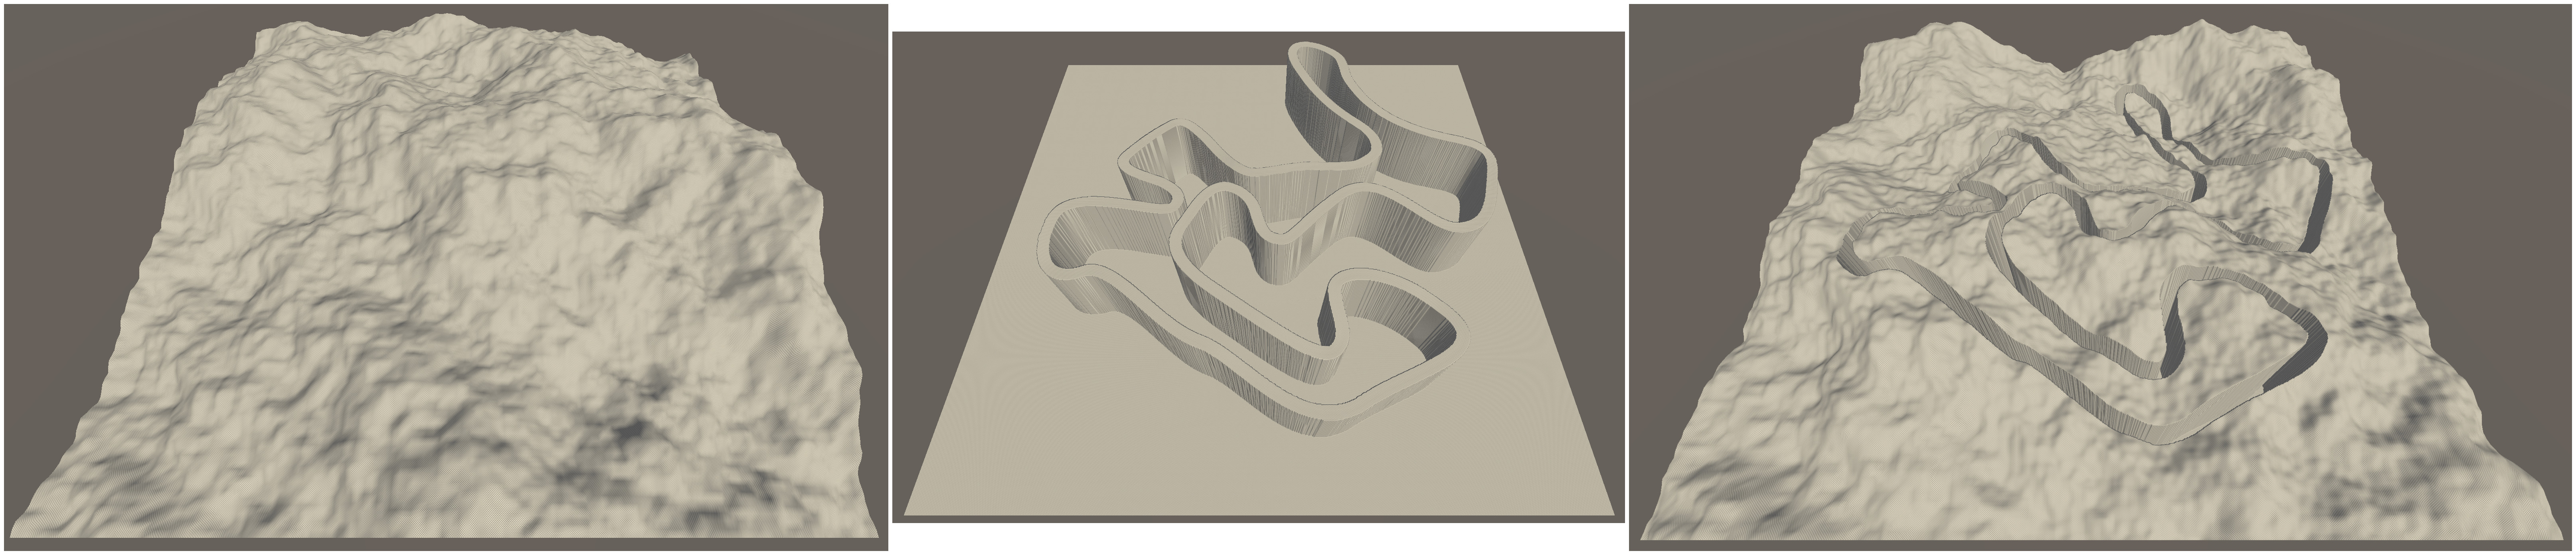
\includegraphics[width=1.0\textwidth]{img/discontinuity_example.jpg}
    \caption{Conceptual illustration of the boundary problem in constrained procedural generation. (Left) Unconstrained terrain generated with Perlin noise. (Centre) Fixed height constraints embedded in the terrain. (Right) The resulting discontinuities that appear at the boundaries between fixed and procedurally generated areas.}
    \label{fig:constraint_discontinuity}
\end{figure}

When we place fixed height areas inside generated terrain without proper blending, obvious breaks appear where they meet. These artifacts destroy the visual coherence of the terrain and create unrealistic formations, like sudden cliffs or unnatural slopes. Developing techniques to address this boundary problem is a central focus of our research.


\subsection{Previous Approaches to Constrained Generation}

Conventional procedural terrain generation typically starts from a flat surface and then populates the heightmap with elevations derived from generative algorithms, such as Perlin noise and midpoint displacement. The output of the algorithm is controlled by fine-tuning various parameters (for example, the maximum height allowed), but overall does not allow for very precise control.  This is where many have used the concept of \textit{constrained procedural generation}. These approaches do not necessarily tackle the exact same problem as we intend to, where these constraints are the fixed heights of any areas in the terrain. Rather, they tend to be more \textit{specific} to a type of constraint, such as generating surrounding terrain for a \textbf{predefined} river network. We will now discuss current existing solutions to this problem. 

\subsubsection{The Bottom-Up Method}
\label{bottom_up_method}

The \textbf{bottom-up approach} for procedural generation, described by \textcite{Belhadj07,} starts with the constraints themselves as the foundation for terrain growth, building \textit{outward} from these fixed points. This method is designed to work well when constraints form connected patterns like river networks or ridge lines, as these constraint types are continuous paths through the terrain rather than isolated points.

This solution works by storing the heights and areas of the river network in a digital heightmap while all other points remain to be computed afterwards. To address the boundary problem, \textcite{Belhadj07} developed their novel \textbf{Midpoint Displacement Inverse (MDI)} process, which inverts the traditional midpoint displacement operation to propagate height information outwards from the fixed points, creating smooth transitions to the surrounding procedurally generated terrain.

While this approach produces realistic terrain without discontinuities, it may not work well with \textbf{isolated fixed points}. Additionally, the method is tailored to midpoint displacement and does not readily apply to other procedural terrain generation methods. 

\subsubsection{Path-Based Constraint Methods}
\label{path_based_method}

Another method addressing the constraint problem is described in the paper  \citetitle{Andereck14}, where the author focuses specifically on \textbf{path constraints}. In this work, \textit{user-defined paths} with exact height constraints serve as the foundation for terrain generation. Unlike approaches that may modify constraints slightly for better terrain coherence, this method preserves the exact heights of predefined paths while procedurally generating surrounding terrain features.

The algorithm employs a data structure that works with multiple different scales. At each scale of the data structure, the algorithm fits planes to constraint points using least-squares fitting, ensuring the terrain naturally conforms to the paths while maintaining realistic slopes. This creates terrain that respects path heights while achieving smooth transitions to the surrounding areas.

This approach works particularly well for path-like constraints but is less suitable for \textbf{arbitrary} fixed areas or disconnected constraint patterns \footnote{We will demonstrate a comparison between our approach and both bottom-up and path-based methods in Chapter \ref{Chapter5}.}.

While these constrained generation methods provide mechanisms for integrating fixed height areas with procedurally generated terrain, they introduce an additional layer of complexity that extends beyond the boundary problem itself. Each technique requires careful parameter tuning to achieve natural-looking results, and when multiple techniques are combined in complex pipelines, the parameter optimisation challenge becomes a significant barrier to practical adoption. The following section examines this fundamental challenge and explores algorithmic approaches for addressing it.

\section{Parameter Optimisation in Procedural Generation}
\label{parameter_optimization}

While constrained procedural generation methods provide mechanisms for integrating fixed height areas with generated terrain, they introduce a fundamental challenge that extends beyond the boundary problem: \textbf{parameter optimisation}. Each terrain generation technique brings its own set of parameters that must be carefully tuned to achieve desired results. When these techniques are combined in complex pipelines, the parameter space becomes vast and interconnected, creating a significant barrier to effective terrain generation.

Consider a typical terrain generation pipeline that might include Perlin noise (requiring frequency, octaves, persistence, and amplitude parameters), Voronoi-based mountain generation (needing peak count, falloff rates, and height ranges), multiple smoothing operations (each with iteration counts and strength parameters), and erosion simulations (requiring threshold values and erosion rates). When these operations are chained together, the parameter space becomes \textbf{exponentially complex}, with small changes in one parameter often requiring adjustments throughout the entire pipeline to maintain natural-looking results.

This parameter complexity represents one of the most significant practical challenges in procedural content generation. Traditional approaches require either expert domain knowledge for manual tuning or mathematical fitness functions for automated optimisation, both of which are problematic when the goal is subjective terrain quality that depends on aesthetic preferences rather than quantifiable metrics.

\subsection{The Parameter Space Challenge}
\label{parameter_space_challenge}

The complexity of parameter tuning in procedural terrain generation manifests in several ways. \textbf{Parameter interdependency} means that adjusting one parameter often requires compensatory changes throughout the system. For example, increasing noise amplitude might necessitate stronger erosion and different smoothing parameters to maintain realistic terrain characteristics. This makes systematic exploration difficult and counter-intuitive. Furthermore, \textbf{subjective quality assessment} presents a fundamental difficulty. Unlike optimisation problems with clear mathematical objectives, terrain quality is \textit{inherently} aesthetic and context-dependent. What constitutes "natural" or "appealing" terrain varies significantly based on the intended application, user preferences, and specific environmental context.


These challenges motivate the need for alternative optimisation approaches that can navigate complex parameter spaces while incorporating human aesthetic judgment. Genetic algorithms, particularly in their interactive variants, provide a promising framework.

\subsection{Genetic Algorithms: Fundamentals}
\label{genetic_algorithms_fundamentals}

\textbf{Genetic algorithms} (GAs) represent a class of evolutionary computation techniques that mimic the process of natural selection to solve optimisation and search problems. Unlike traditional methods that rely on gradient information, GAs maintain a \textbf{population} of candidate solutions and evolve them through \textbf{selection}, \textbf{crossover}, and \textbf{mutation}.

In terrain generation, an \textbf{individual} (of the population) might represent a \textit{specific combination} of algorithm parameters. Additionally: 

\begin{itemize}
    \item The \textbf{fitness function} measures \textit{how well} an individual solves the problem. Higher-fitness individuals are more likely to be selected for reproduction; 
    \item \textbf{Elitism} ensures the best individuals are preserved throughout the whole evolutionary process;
    \item \textbf{Crossover} combines traits from parents;
    \item \textbf{Mutation} introduces random variations in the individuals.
\end{itemize}

One complete cycle of the algorithm consists of all these features (usually ordered as: evaluation, selection, crossover, and mutation). The algorithm iterates through multiple generations, with the population gradually improving over time.

\subsection{Interactive Genetic Algorithms}
\label{interactive_genetic_algorithms}

While traditional genetic algorithms rely on mathematical fitness functions, many creative and design problems, including terrain generation, involve subjective quality criteria that resist formal mathematical description. \textbf{Interactive Genetic Algorithms} (IGAs) address this limitation by replacing automated fitness evaluation with \textbf{human judgment}, transforming the optimisation process into a collaborative exploration between human creativity and algorithmic efficiency. 


Interactive genetic algorithms also introduce unique challenges that distinguish them from traditional automated approaches. Human evaluation is limited by attention span and cognitive load, so IGA systems must balance population size and generation length to avoid user fatigue. A common approach is to let users select multiple preferred individuals, instead of scoring each one numerically.

The IGA approach has been applied to terrain generation by \textcite{Walsh10}, who developed a system where users evolved terrain through visual selection. Their work demonstrated that users could discover appealing parameter combinations without needing detailed technical knowledge. 


\hfill

Inspired by this work and motivated by existing challenges and limitations, we build on this framework and present our solution via an interactive genetic algorithm in Chapter \ref{Chapter4}. Together, these innovations provide a practical and efficient method for procedural terrain generation with fixed height constraints.



\chapter{System Design and Architecture}
\label{Chapter2}

This chapter presents the design and architecture of our constrained procedural terrain generation system. Building upon the limitations of existing approaches identified in Chapter \ref{Chapter1}, we develop a modular system that addresses the key challenges through a \textbf{distance-based} methodology.

We first establish our system requirements and design objectives, then detail the component-based architecture that enables flexible combinations of terrain operations. We explain our overall workflow and conclude with Unity-specific implementation considerations. The mathematical foundations of our distance-based approach are detailed in Chapter \ref{Chapter3}, while the Interactive Genetic Algorithm for parameter optimisation is covered in Chapter \ref{Chapter4}.

\section{System Requirements and Design Goals}

In response to the challenges discussed in previous sections, we established the following system requirements and design goals to guide the development of our terrain generation framework.

\subsubsection{Core Requirements}

\begin{itemize}
    \item \textbf{Constraint Preservation}: Fixed points must maintain their exact heights throughout the generation process -- we never modify the heights of these areas. We use \textbf{mask} \textbf{textures} where red pixels indicate fixed areas and black pixels represent modifiable regions. This intuitive format integrates well with standard image editing tools (see Figure \ref{fig:mask_examples});

    \item \textbf{Natural Transitions}: The system should create \textit{smooth, realistic transitions} between fixed and generated terrain, avoiding the abrupt discontinuities that typically occur when applying traditional procedural techniques to constrained problems; 

    \item \textbf{Algorithmic Flexibility}: The architecture should accommodate \textit{a variety} of terrain generation techniques without requiring algorithm-specific modifications for constraint handling. This enables integration of Perlin noise, Voronoi Diagrams, and Midpoint Displacement methods.
    
\end{itemize}

\subsubsection{Design Objectives}

Based on these requirements, we defined the following five key objectives:

\begin{itemize}
    \item \textbf{Modular Architecture}: Enable flexible combinations of terrain operations using a component-based design that cleanly separates responsibilities;
    
    \item \textbf{Distance-Based Processing}: Use proximity to fixed points to guide terrain modifications;
    
    \item \textbf{Intuitive Parameter Tuning}: Provide both manual control and automated parameter exploration through Interactive Genetic Algorithms;
    
    \item \textbf{Performance Optimisation}: Leverage GPU acceleration for computationally intensive operations;
    
    \item \textbf{Extensibility}: Allow easy addition of new terrain operations and constraint types.
\end{itemize}

These objectives ensure our system serves both novice users seeking accessible terrain generation and expert users requiring precise control.

\subsubsection{Architectural Approach}
\label{top_down_approach}

We adopt a \textbf{top-down approach}, in which we first generate the entire terrain using traditional methods, and then adjust it to respect the given constraints. Specifically, in the modifiable areas (represented by black pixels in the mask), we initially run the procedural terrain generation algorithms without considering the constraints. This is illustrated in Figure \ref{fig:top_down_example}, where the constrained regions remain untouched and do not yet influence the surrounding terrain. 


\begin{figure}[h!]
    \centering
    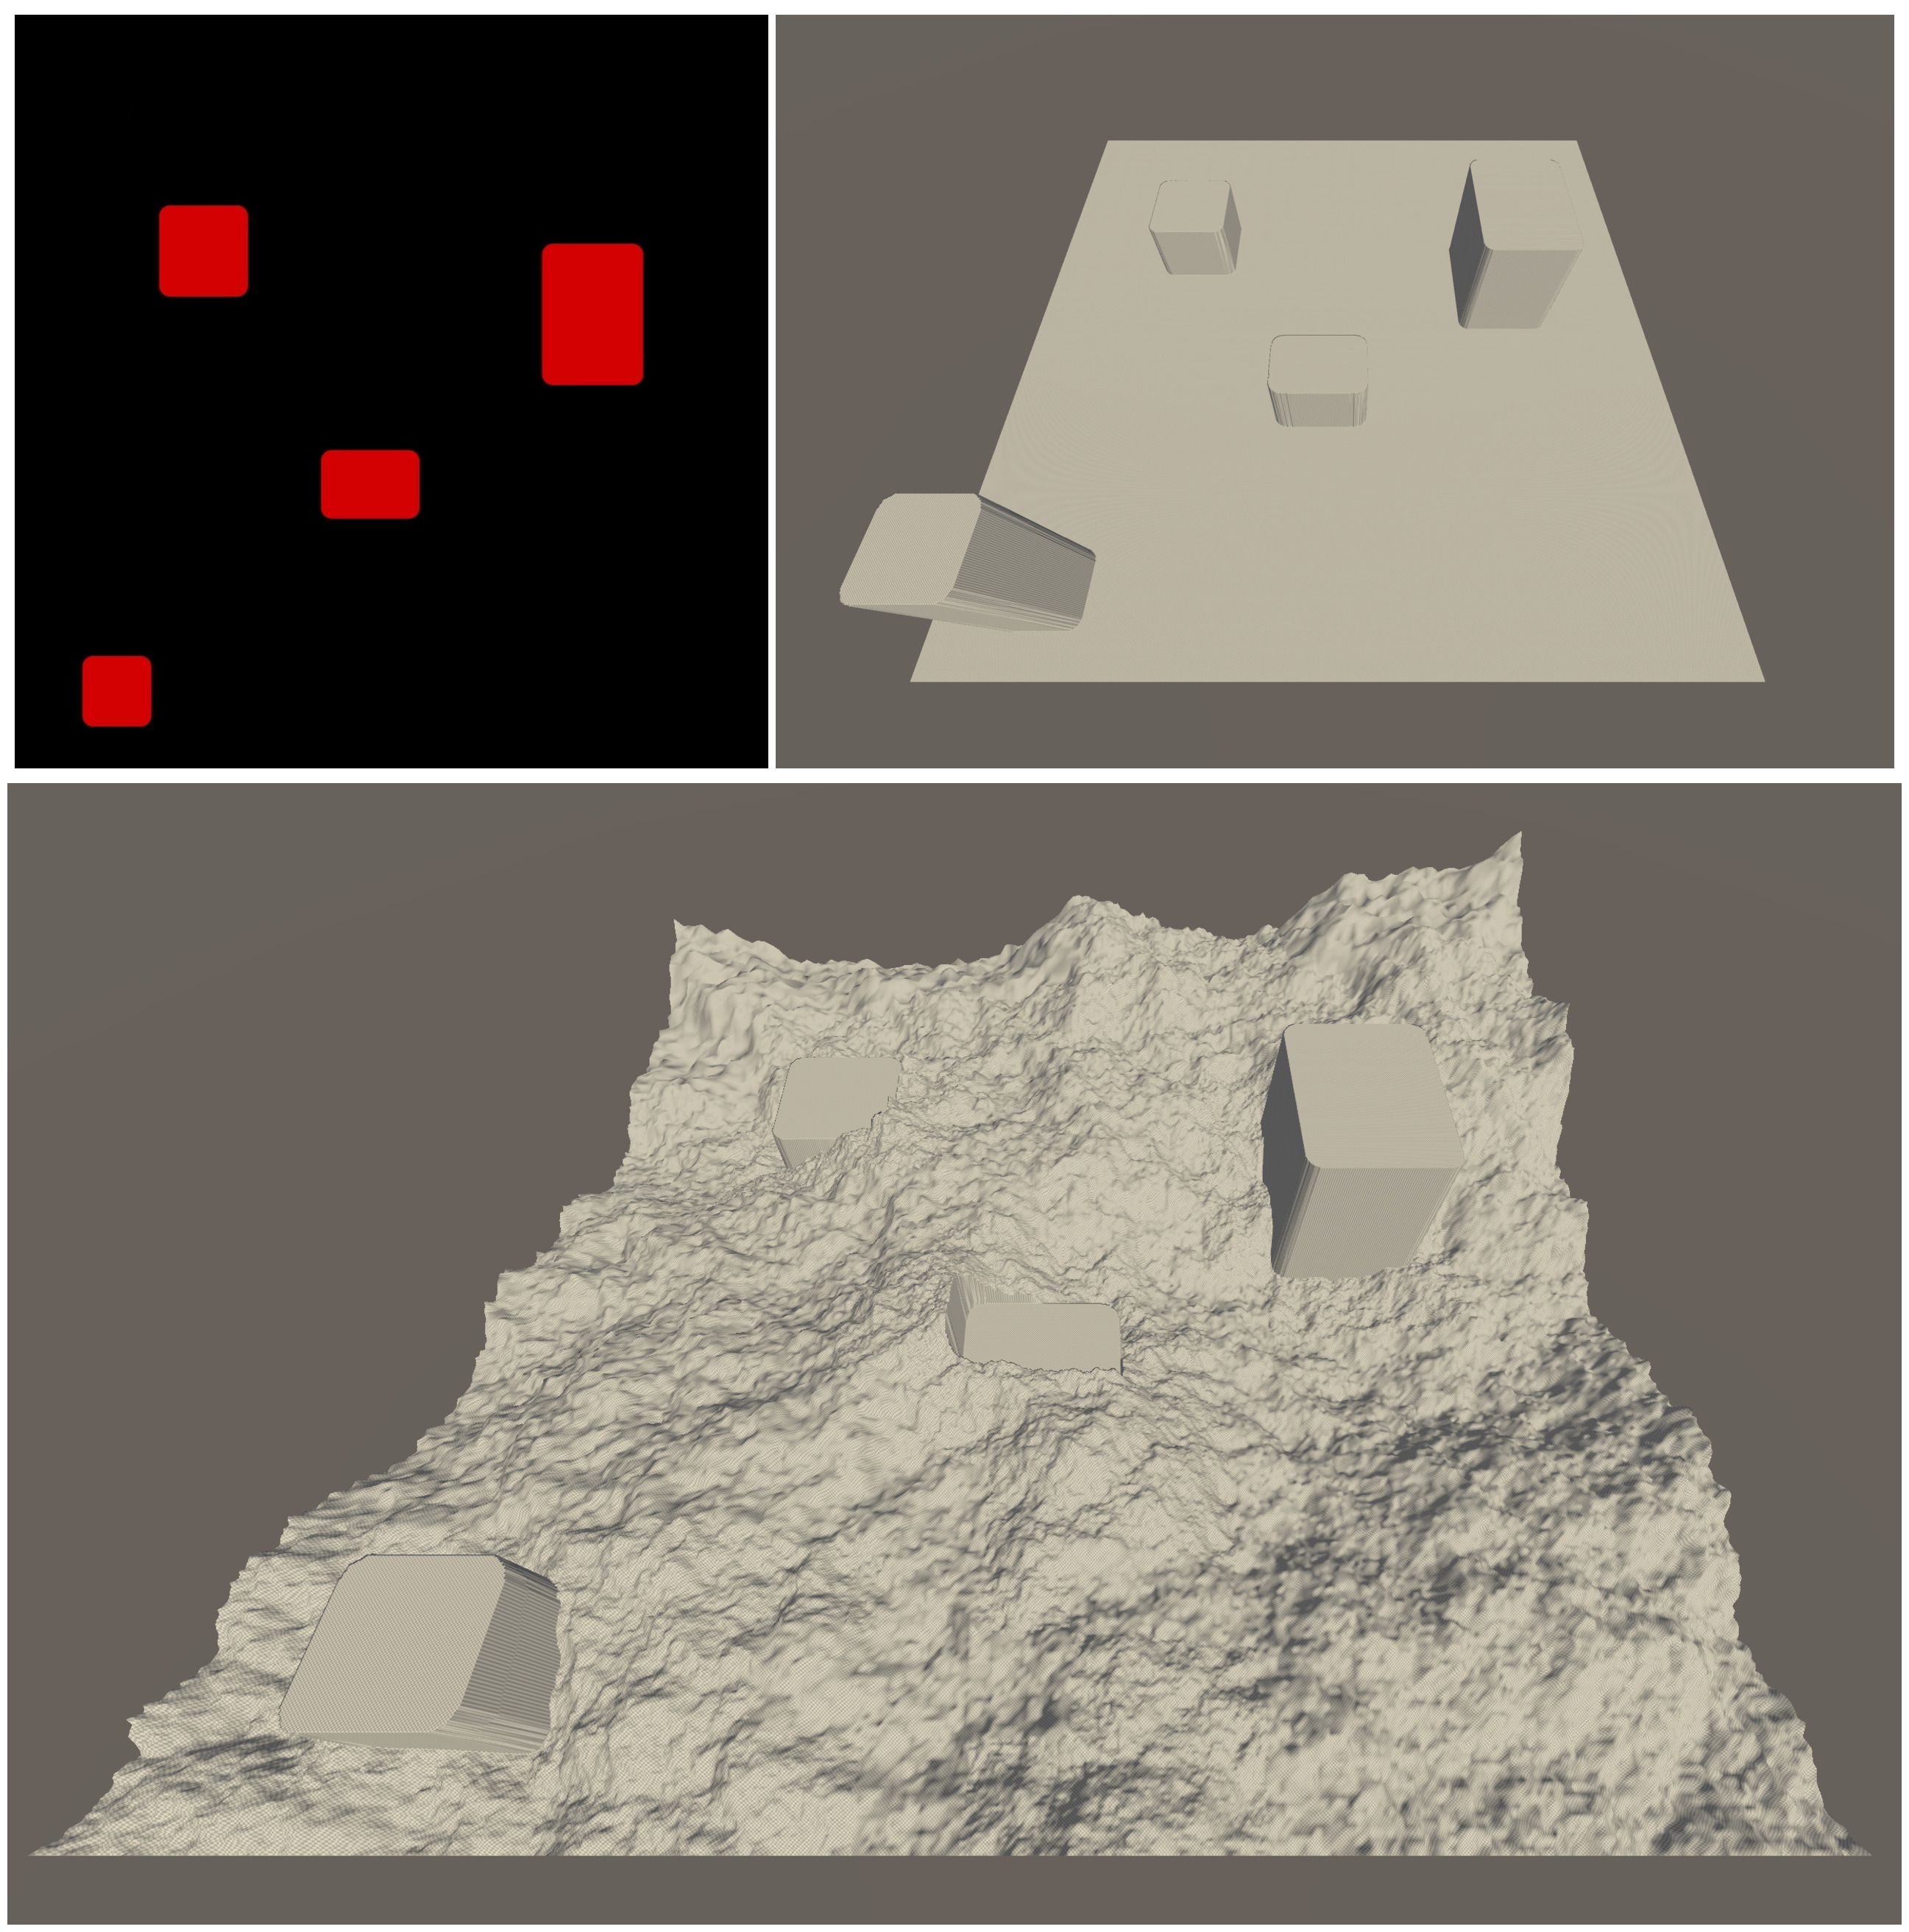
\includegraphics[width=0.7\linewidth]{img/Chapter_2_images/building_example_top_down.jpg}
    \caption{\textbf{Top left} Shows the mask texture, with red pixels indicating constrained areas, and black pixels indicating modifiable areas; \textbf{top right} shows the predefined heights of the constrained areas in the terrain, and all the modifiable pixels heights are currently set to 0; \textbf{bottom figure} shows resulting terrain after running midpoint displacement algorithm, before applying any post-processing to smooth out transitions.}

    \label{fig:top_down_example}
\end{figure}

In the second step, we apply \textbf{post-processing} to modify the surrounding terrain so that it blends smoothly into the constrained areas (identified by red pixels in the mask).

This contrasts with the \textbf{bottom-up} methods that propagate constraints outward from fixed points using \textit{Inverse Midpoint Displacement} \citep{Belhadj07}. Our approach offers greater flexibility and compatibility with existing algorithms, requiring only that operations respect the constraint mask, rather than implementing specialised \textit{constraint-aware} algorithms.

This architectural decision profoundly influences our system design, enabling the modular, component-based structure that separates constraint handling from specific terrain generation techniques.

\section{Component-Based Architecture}
In this section we describe the actual component-based architecture of our system. We can see a visual representation of this structure in the diagram in Figure \ref{fig:component_diagram} below.

\begin{figure}[h!]
    \centering
    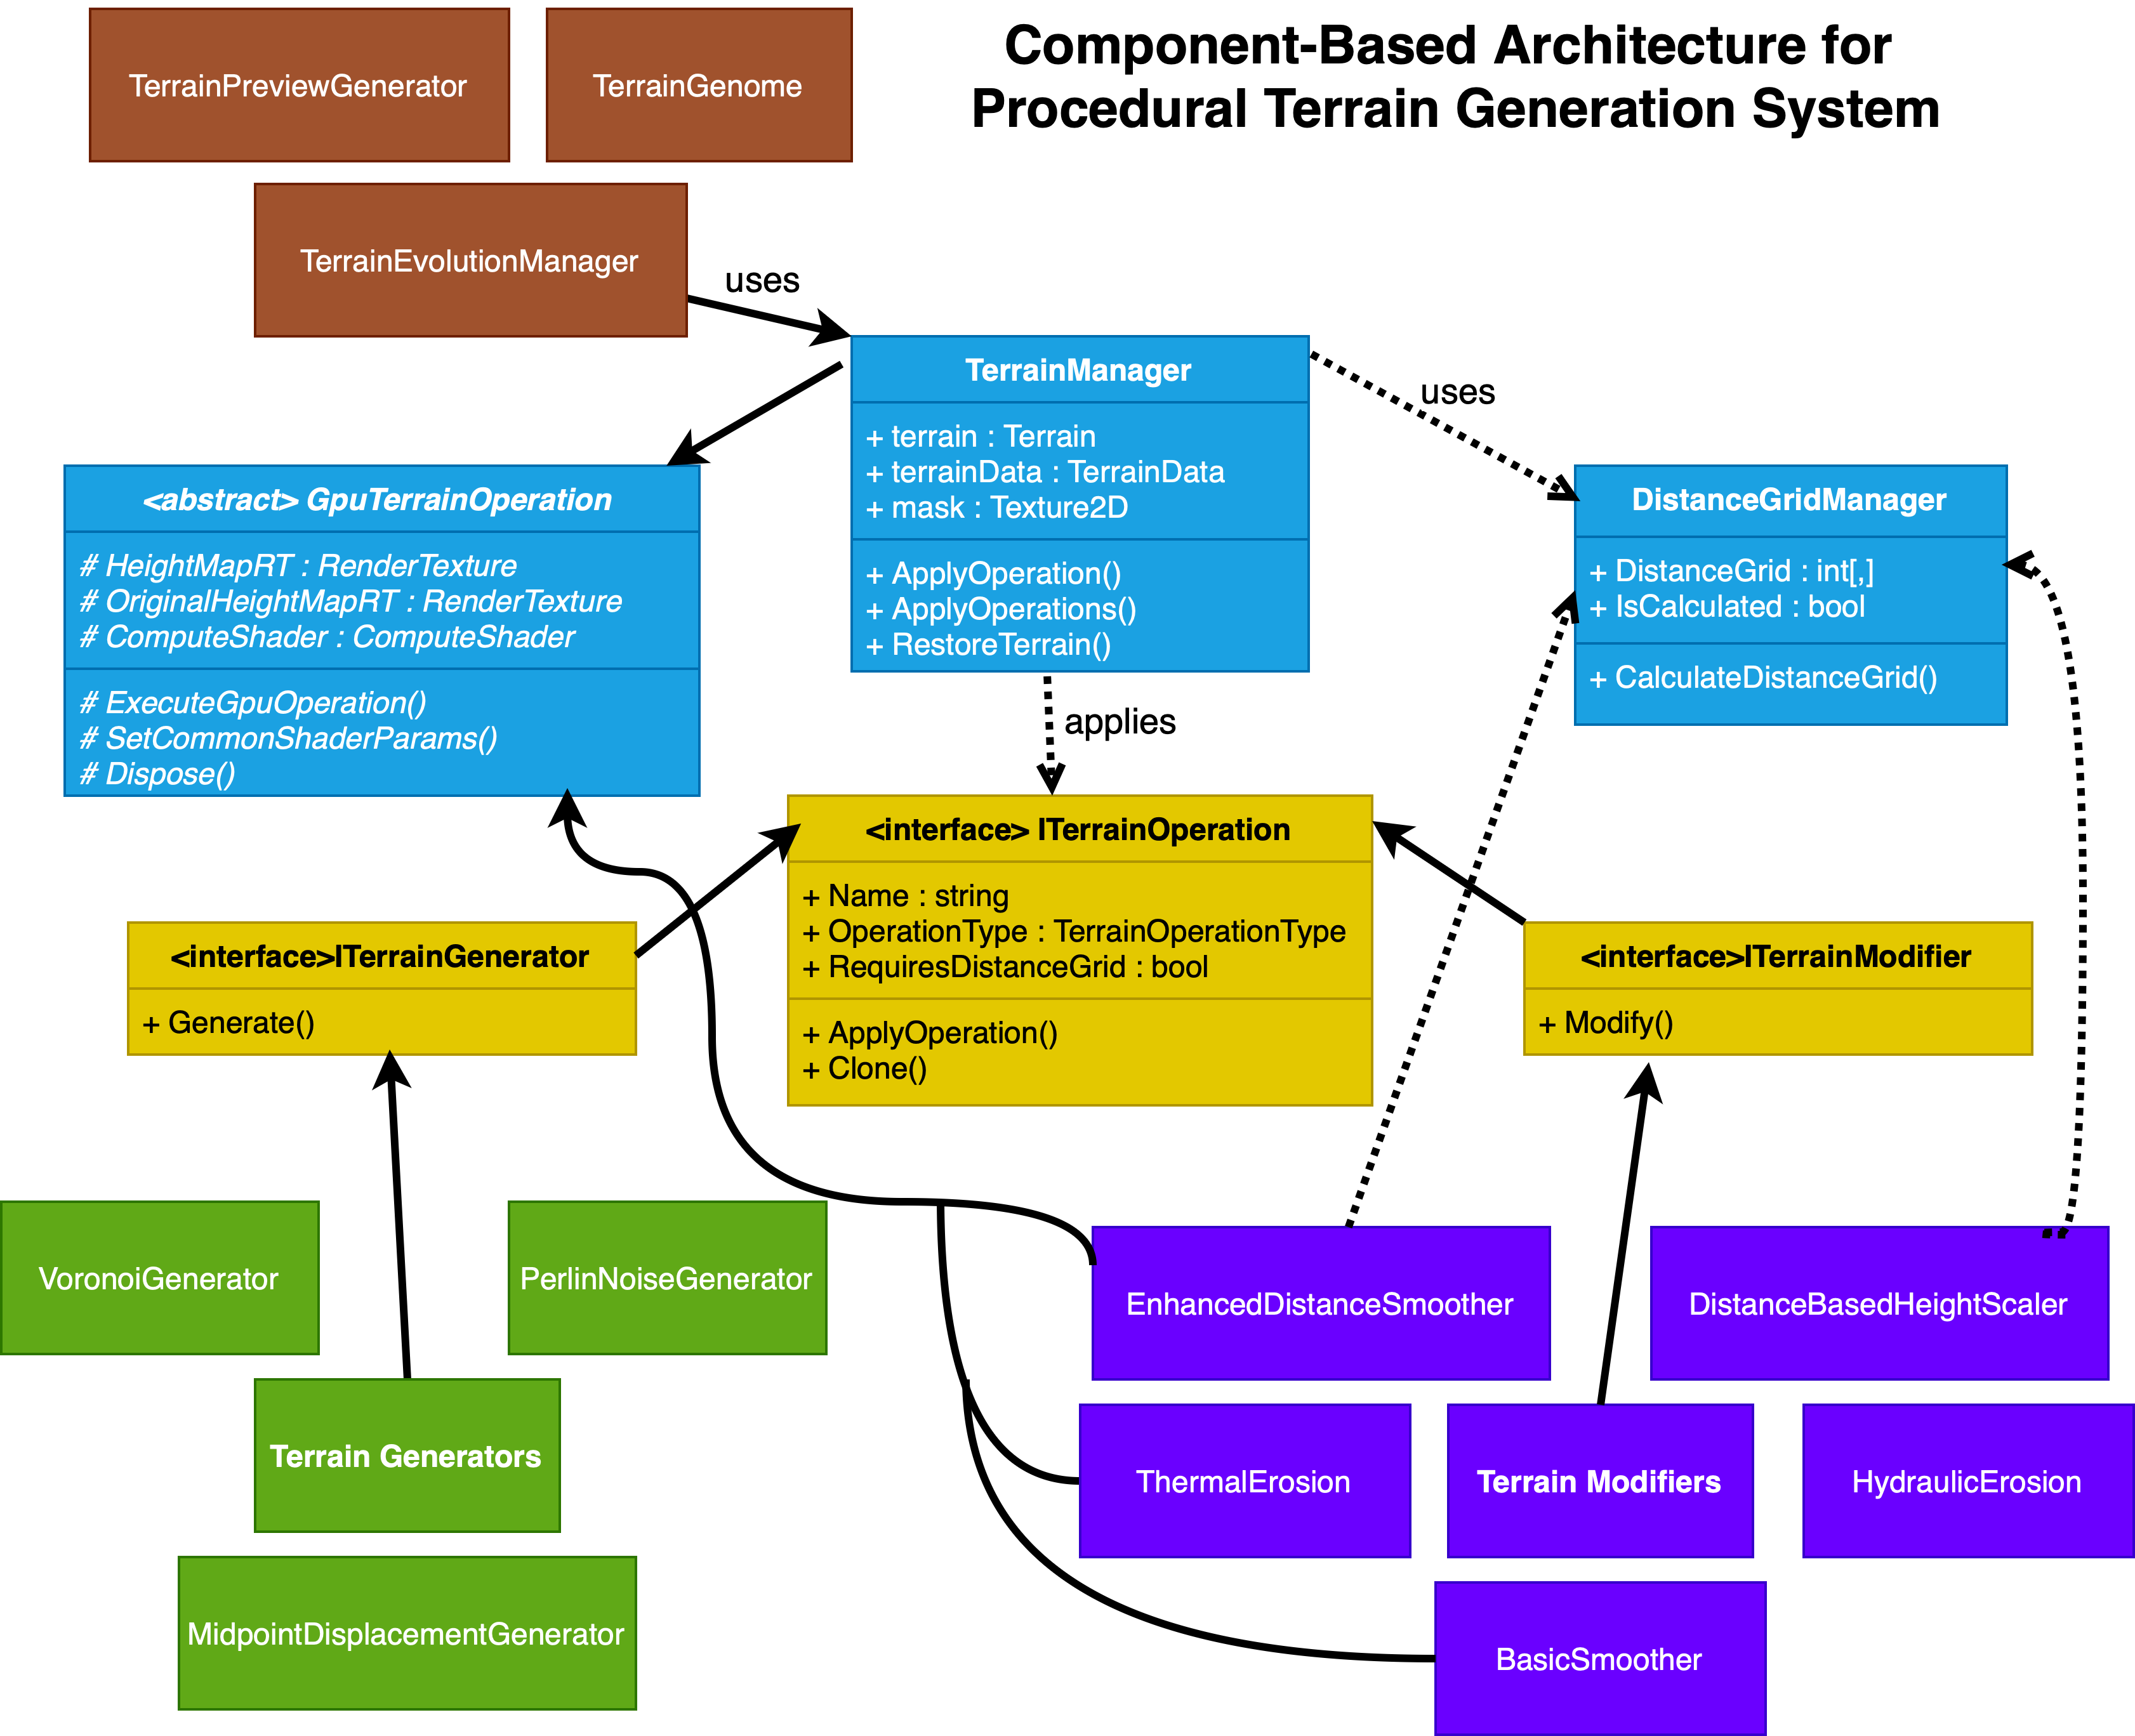
\includegraphics[width=1.0\textwidth]{img/Chapter_2_images/Diagrams/component_diagram.png}
    \caption{High-level architecture showing core components and relationships. The \textsf{TerrainManager} coordinates operations, while \textsf{ITerrainOperation} implementations provide specific algorithms to change the heights of modifiable areas in the terrain. \textsf{DistanceGridManager} supplies proximity information for distance-aware operations. \textsf{TerrainEvolutionManager} is how the IGA connects to the system. }
    \label{fig:component_diagram}
\end{figure}

% \subsection{Core Components}
Specifically, each component does the following:

\textbf{\textsf{TerrainManager}}: The central coordinator that manages Unity terrain objects, interprets constraint masks, and applies operations while preserving fixed heights. This component serves as the \textbf{primary interface} for both manual operation and IGA-based approaches.
    

\textbf{\textsf{ITerrainOperation} Interface}: All terrain operations implement this foundational interface, which defines the essential \textit{contract} for terrain modification. The interface specifies operation methods, distance grid requirements, and support for genetic algorithm operations through cloning.

Operations are categorised as either \textsf{ITerrainGenerator} (create terrain features) or \textsf{ITerrainModifier} (adjust existing terrain). This distinction aids organisation and user interface design, though both types follow the same operational pattern.
    
\textbf{\textsf{DistanceGridManager}}: Calculates and maintains distance information from each terrain point to the nearest fixed point using an efficient breadth-first search algorithm. This component enables distance-aware operations, forming a crucial part of our distance-based methodology (see Chapter \ref{Chapter3}).


\textbf{\textsf{GpuTerrainOperation}}: Base class for GPU-accelerated operations, handling compute shader management and CPU/GPU data transfer. This component provides automatic fallback to CPU implementations when GPU acceleration is unavailable. Technical implementation details are available in our system's source code.

\subsubsection{Operation Pipeline}

Our system applies operations \textbf{sequentially}, with each additional operation building upon the results of previous one. This pipeline approach enables:
\begin{itemize}
    \item Explicit control over operation ordering;
    \item Independent parameter adjustment for each operation;
    \item Easy experimentation with different operation combinations;
    \item Natural integration with genetic algorithm mutations and crossover.
\end{itemize}

The pipeline accommodates the full range of terrain operations available in our system. Complete parameter descriptions are available in the user documentation, while implementation specifics can be found in the source code.

\subsubsection{User Interaction Models}
\label{interaction_models}

Our architecture supports two distinct interaction approaches that serve different user needs and expertise levels:


\begin{itemize}
    \item \textbf{Manual Operation Approach}: Users directly select and configure terrain operations through Unity's inspector interface. This approach provides:
\begin{itemize}
    \item[-] Precise control over individual operation parameters;
    \item[-] Direct manipulation of operation sequences;
    \item[-] Immediate visual feedback for iterative refinement;
    \item[-] Full access to the complete parameter space for expert users.
\end{itemize}

This method suits users with terrain generation expertise who require fine-grained control over the generation process.

    
    \item \textbf{Interactive Genetic Algorithm Approach}:
The system generates populations of terrain variants with different operation sequences and parameters, allowing users to guide evolution through visual selection rather than manual parameter tuning. This approach, based on the pioneering work by \textcite{Walsh10}, enables:
\begin{itemize}
    \item[-] Intuitive exploration of complex parameter combinations;
    \item[-] Discovery of aesthetically pleasing solutions without technical expertise;
    \item[-] Guided evolution through user aesthetic preferences;
    \item[-] Accessible terrain generation for non-expert users\footnote{The complete IGA implementation and methodology are detailed in Chapter \ref{Chapter4}.}.
\end{itemize}

\end{itemize}

\section{Workflow Overview}

\begin{figure}[h!]
    \centering
    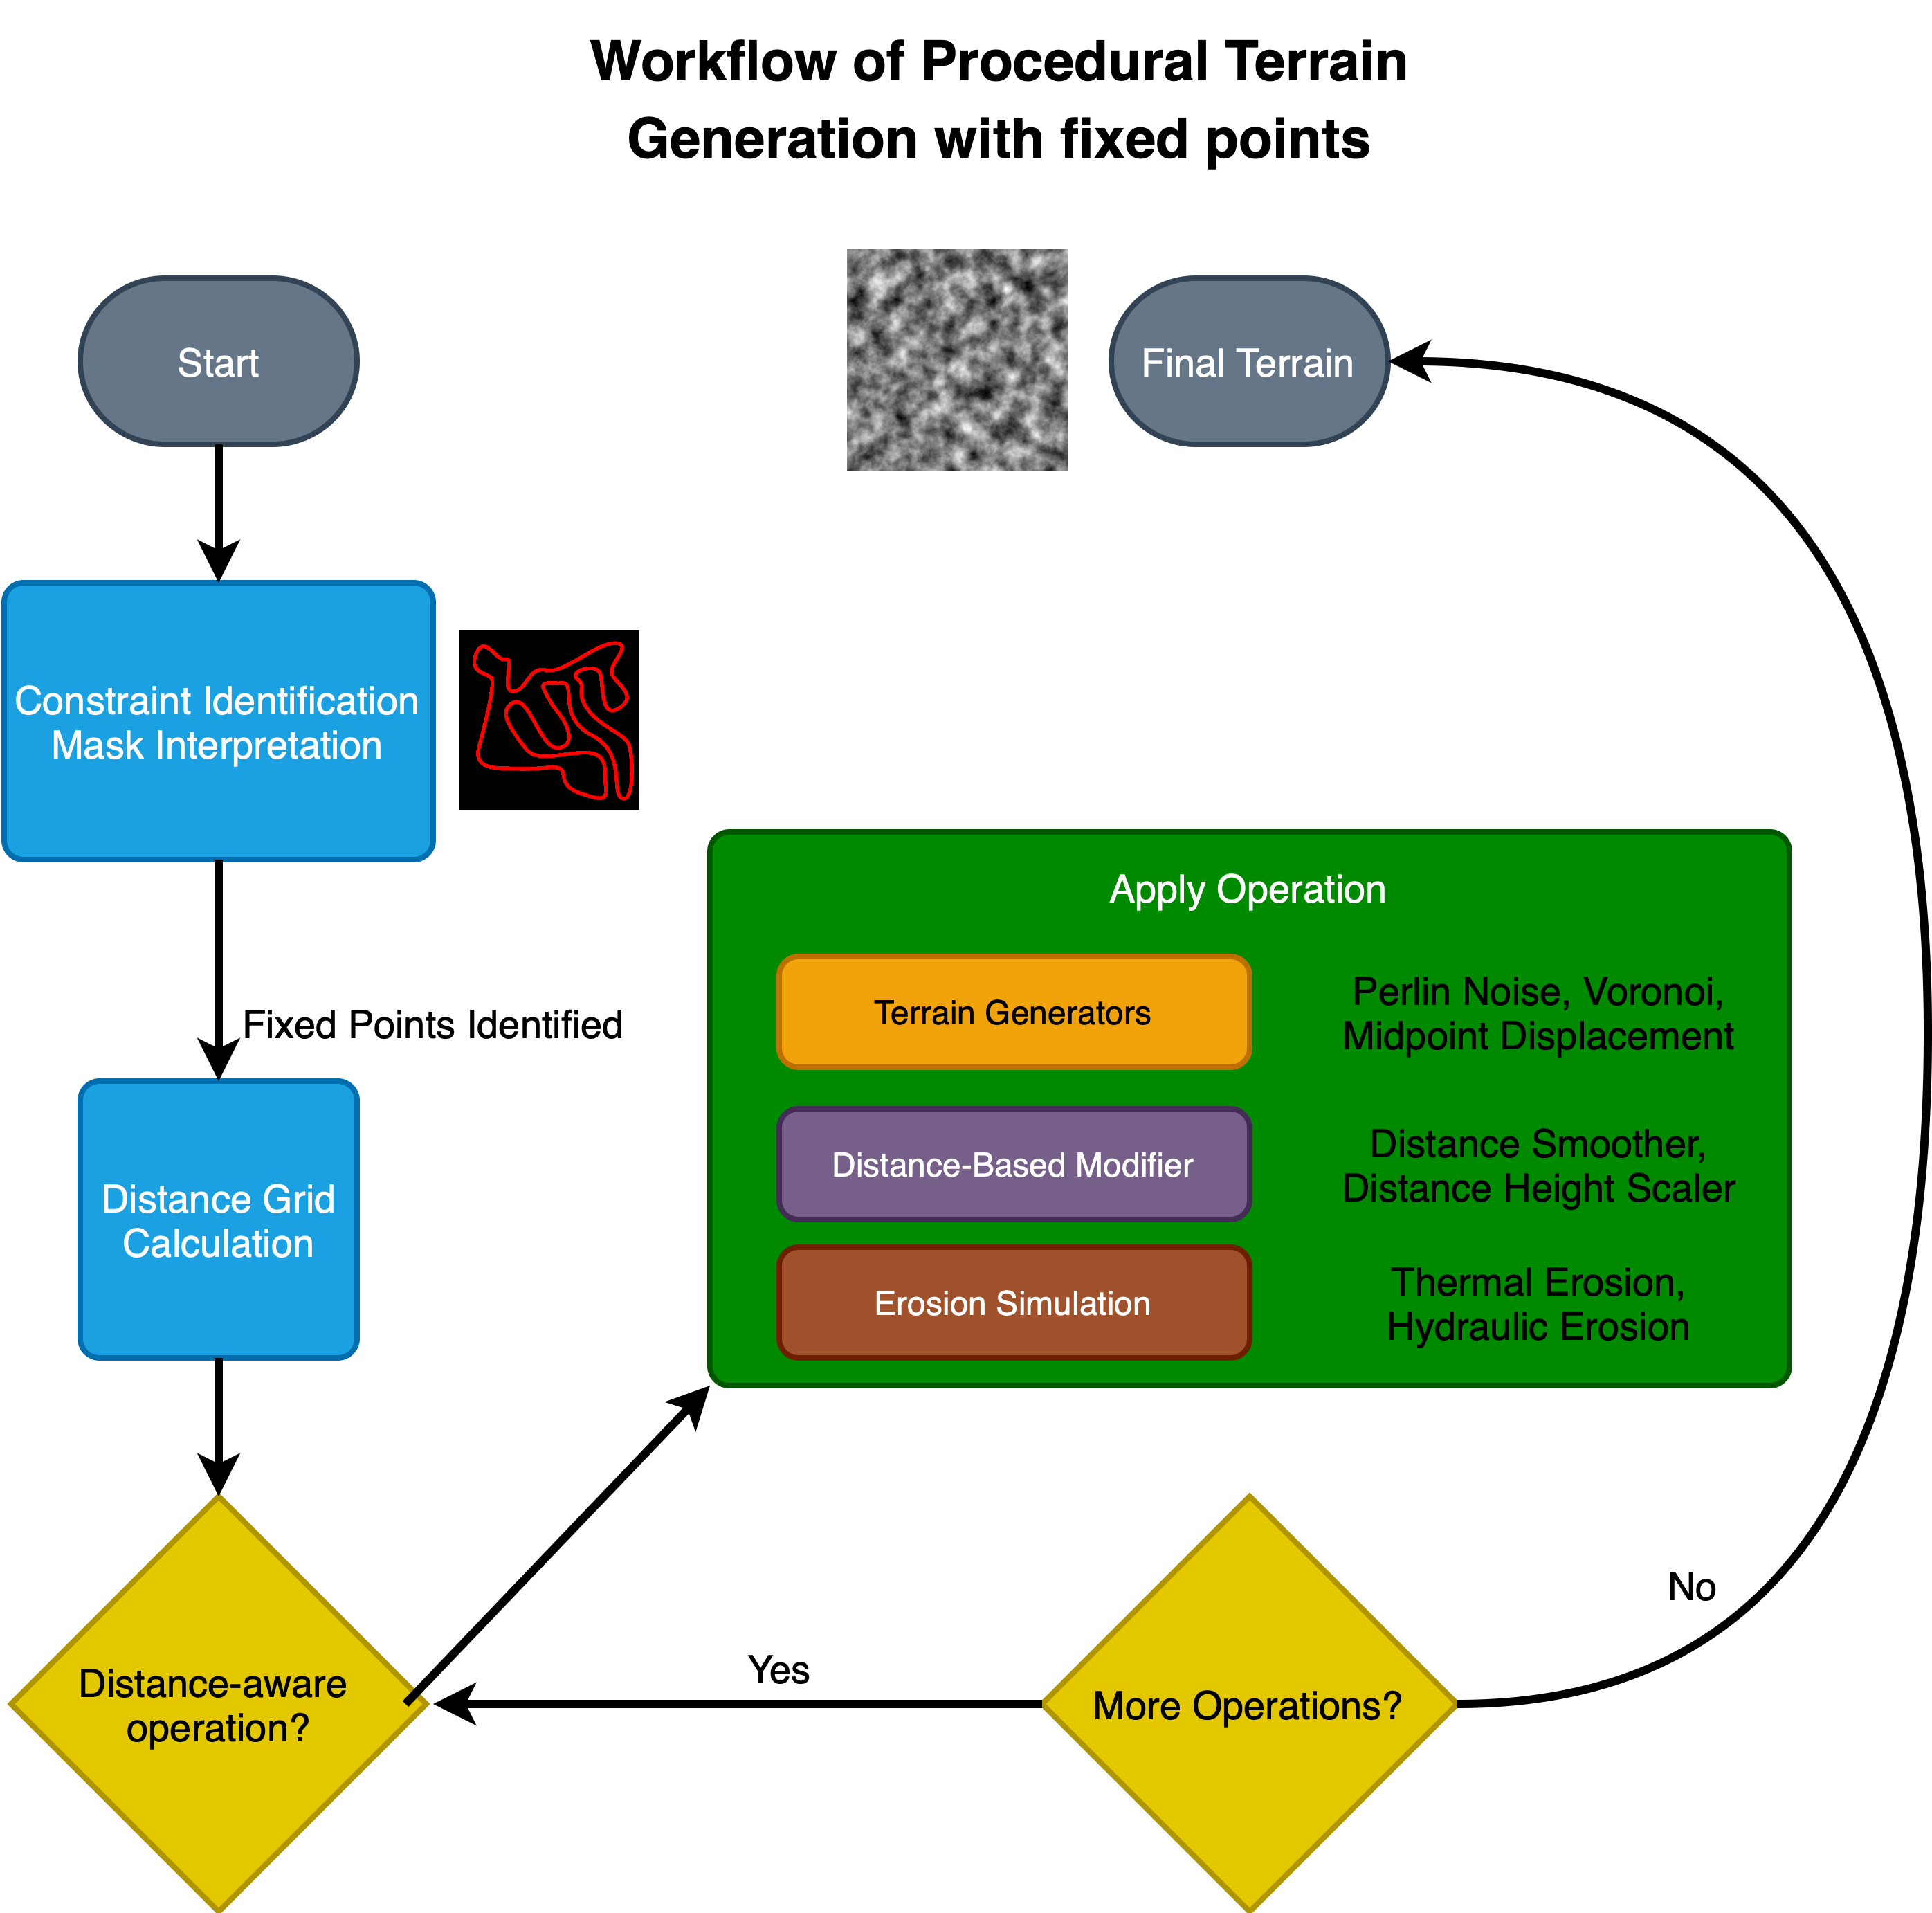
\includegraphics[width=1.0\textwidth]{img/Chapter_2_images/Diagrams/workflow_diagram.png}
    \caption{System workflow from constraint identification through terrain generation and modification. Distance grid calculation enables distance-aware operations to create natural transitions between fixed and generated areas.}
    \label{fig:workflow_diagram}
\end{figure}

Our system follows a five-stage workflow that transforms initial constraints into natural-looking terrain. A visual representation of this workflow can be seen in Figure \ref{fig:workflow_diagram}. This workflow is exactly the same whether users employ manual operation selection or the Interactive Genetic Algorithm approach.

\subsubsection{Constraint Identification}
\label{mask_interpretation}

The workflow begins with identifying fixed areas through mask textures. As we mentioned above, red pixels represent immutable heights, while black pixels indicate modifiable regions. 

\begin{figure}[h!]
    \centering
    
\includegraphics[width=0.8\textwidth]{img/Masks/mask_example.jpg}
    \caption{Example constraint masks representing different scenarios: racing track layout (left) where roads maintain fixed heights, and island coastline (right) where water levels remain constant. Red areas preserve exact heights while black areas allow procedural modification.}
    \label{fig:mask_examples}
\end{figure}

The mask interpretation system handles arbitrary constraint patterns, from simple geometric shapes to complex networks. This flexibility enables applications ranging from road integration to architectural site planning.

\subsubsection{Distance Grid Calculation}

For operations requiring distance information, the system calculates the minimum distance from each terrain point to the nearest fixed point. This distance grid enables adaptive terrain modifications that create natural transitions by varying operation strength based on proximity to constraints.

The \textsf{DistanceGridManager} component implements this calculation using an efficient breadth-first search algorithm. The mathematical foundations and algorithmic details are presented in Section \ref{distance_grid_calculation}.

\subsubsection{Terrain Generation}

Base terrain creation employs the procedural techniques examined in Section \ref{ptg_fundamentals} including Perlin noise with fractional Brownian motion, Voronoi-based generation, and midpoint displacement. All generators respect the constraint mask by only modifying points marked as modifiable.

Users can combine multiple generation techniques in sequence, with each operation building upon previous results while maintaining constraint awareness throughout the process.


 \subsubsection{Distance-Based Modification}

The system applies distance-aware operations that use proximity to fixed points to guide terrain modifications. Our approach employs two key techniques:

\begin{itemize}
    \item \textbf{\textit{Distance-Based Height Scaling}}: Reduces elevation differences near constraints to prevent cliff formations. This technique gradually blends heights based on distance from fixed points, creating realistic grading around constrained areas. A formal explanation can be seen in Section \ref {dbhs};
    \item \textbf{\textit{Enhanced Distance-Based Smoothing}}: Applies stronger smoothing near fixed points while preserving detail at distance. This creates natural blending without sacrificing terrain character in unconstrained areas. A formal explanation can be seen in Section \ref{edbs}. 
\end{itemize}

\subsubsection{Erosion and Detail Enhancement}

Optional erosion algorithms, as explained in Section \ref{erosion_1}, add realistic weathering effects while respecting constraint boundaries:

\begin{itemize}
    \item \textbf{\textit{Thermal Erosion}} simulates material slumping to create more natural slopes, preventing unrealistically steep terrain formations while maintaining fixed point constraints; 
    
    \item \textbf{\textit{Hydraulic Erosion}} simulates water flow effects to add valley formation and surface detail, enhancing visual realism without compromising constraint preservation.

\end{itemize}

\section{Implementation in Unity}

Our system integrates deeply with Unity's terrain system and editor tools, providing a familiar interface for terrain artists while adding constrained generation capabilities.

\subsection{Terrain System Integration}
\label{terrain_system_integration}

The \textsf{TerrainManager} component attaches to Unity Terrain objects, accessing ``Terrain Component'' \citep{UnityTerrainDocs} to modify heightmaps programmatically. This approach leverages Unity's existing terrain infrastructure while adding constraint-aware generation capabilities.
Custom editor extensions provide two complementary interfaces:
\begin{itemize}
    \item \textbf{Inspector Interface}: Exposes terrain operations with adjustable parameters for manual control, integrated with Unity's standard component inspector workflow. This is demonstrated in Figure \ref{fig:manual_editor} below.
        \begin{figure}
            \centering
            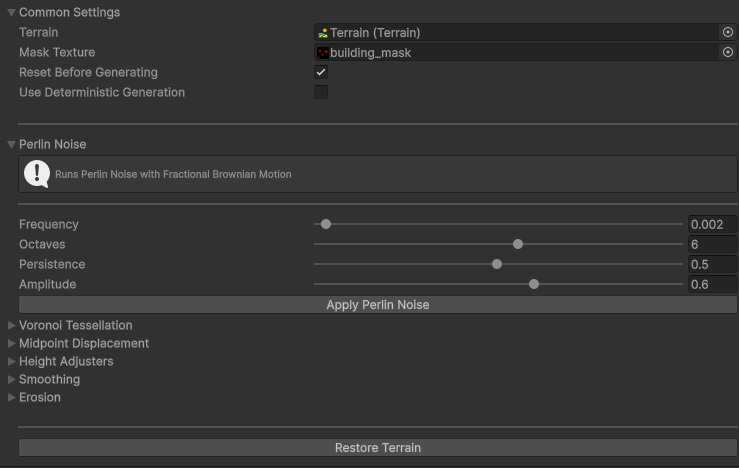
\includegraphics[width=1.0\linewidth]{img/Chapter_2_images/example_editor.png}
            \caption{The custom interface in the Unity inspector, which appears through adding the \textsf{TerrainManager} as a component to the terrain game object. We can see the mask is uploaded here, and it provides a drop-down menu for various operation. In this example, the Perlin noise parameters are shown only, as all the others have a similar layout and level of control over the operations.}
            \label{fig:manual_editor}
        \end{figure}
    \item \textbf{Evolution Window}: Dedicated interface for the Interactive Genetic Algorithm workflow, providing visual terrain variant selection and evolution controls
\end{itemize}

Both interfaces integrate with Unity's ``Extending the Editor'' \citep{UnityEditor} system and undo capabilities, allowing reversible terrain modifications during the design process.

Our system follows Unity's component-based design philosophy, with the \textsf{TerrainManager} serving as the primary component attached to Terrain objects. Additional components like \textsf{TerrainEvolutionManager} enable IGA functionality when needed.


\subsection{GPU Acceleration Implementation}
\label{Gpu_acceleration_2}

To improve performance for computationally intensive terrain operations, our system implements targeted GPU acceleration using Unity's compute shaders. GPU acceleration leverages the parallel processing capabilities of graphics hardware to perform the same operation on thousands of heightmap points simultaneously. We focus acceleration efforts on operations that usually run for multiple iterations, while maintaining robust CPU fallback mechanisms for compatibility and reliability.

\subsubsection{Architecture for GPU-Accelerated Operations}

Our GPU acceleration strategy centres on a unified \textsf{GpuTerrainOperation} base class that handles the complexities of GPU resource management, data transfer, and error handling. This architecture ensures that specific terrain operations can focus on their algorithmic logic while benefiting from consistent GPU acceleration patterns.

The base class manages several critical aspects of GPU processing:

\begin{itemize}
    \item \textbf{Resource Management}: Automatic creation and disposal of GPU textures and compute shader resources;
    \item \textbf{Data Transfer}: Efficient conversion between CPU heightmap arrays and GPU texture formats;
    \item \textbf{Error Handling}: Graceful fallback to CPU implementations when GPU processing fails;
    \item \textbf{Thread Group Organisation}: Standardised 16×16 thread group dispatch for optimal GPU utilisation.
\end{itemize}

This unified approach eliminates code duplication while ensuring consistent performance characteristics across all GPU-accelerated operations in our system.

\subsubsection{Accelerated Operations}

We implement GPU acceleration for three specific terrain operations that demonstrate high computational intensity and excellent parallelisation characteristics. While many other terrain operations could also be GPU accelerated, these three are the only ones that are typically run for multiple iterations, whereas the other operations, such as Perlin Noise, only need to run for a single iteration to achieve good results. The reason for running these three operations over multiple iterations is so that they can have an impactful and significant result on the terrain, where each iteration applies the operation to the resulting terrain of the previous iteration. 

\textbf{Enhanced Distance Smoothing}, as described in Section \ref{edbs}, represents our most sophisticated GPU-accelerated operation. This algorithm applies variable-strength smoothing based on distance from fixed points, requiring complex neighbourhood calculations and distance-aware weighting. The parallel nature of these calculations makes GPU acceleration particularly effective, as thousands of terrain points can be processed simultaneously while accessing distance information from GPU memory. 

\textbf{Basic Smoothing} implements traditional uniform height averaging, where each pixel is set to the average height of all its neighbours, with GPU acceleration. While conceptually simple, this operation benefits substantially from parallel execution when applied to large heightmaps for multiple iterations. 

\textbf{Thermal Erosion}, as described in Section \ref{thermal_erosion}, simulates material slumping through iterative height redistribution. This operation requires multiple passes over the heightmap data, making it an ideal candidate for GPU acceleration due to parallel processing of erosion calculations across all terrain points.

Each operation implements the same interface pattern, accepting heightmap data and constraint information while producing modified terrain that respects fixed height constraints.

\subsubsection{Compute Shader Implementation}

Our compute shaders follow Unity's compute shader system, utilising GPU parallel processing capabilities \cite{UnityComputeShaders}. Each shader kernel processes individual heightmap points within 16×16 thread groups, maximising GPU utilisation while maintaining memory access efficiency.

The compute shader workflow follows this pattern:

\begin{enumerate}
    \item \textbf{Heightmap Upload}: CPU heightmap data is converted to GPU format;
    \item \textbf{Constraint Mask Transfer}: Fixed point constraints are encoded as mask textures;
    \item \textbf{Parallel Processing}: Compute shader kernels process all modifiable points simultaneously;
    \item \textbf{Iterative Refinement}: Multiple passes refine results while respecting constraints;
    \item \textbf{Data Readback}: Final heightmap data is transferred back to CPU memory.
\end{enumerate}

This workflow minimizes CPU-GPU data transfer overhead by keeping data on the GPU throughout multi-iteration operations.

\subsubsection{CPU Fallback Strategy}

Since not all systems support compute shaders or have sufficient GPU capabilities, every GPU-accelerated operation in our system includes a complete CPU fallback implementation. This strategy ensures system reliability across diverse hardware configurations while maintaining identical algorithmic behaviour regardless of the execution platform.

\subsubsection{Integration with Interactive Genetic Algorithm}

GPU acceleration proves particularly valuable for the Interactive Genetic Algorithm approach detailed in Chapter \ref{Chapter4}. The IGA requires rapid generation of multiple terrain variants, making the parallel processing capabilities of GPU acceleration essential for responsive user interaction. Since each terrain operation is now quicker, running multiple of them repeatedly saves a lot of waiting time when generating different variants of the terrain.

Complete technical implementation details, including compute shader source code and resource management patterns, are available in our system's documentation and source code repository.

\section{Summary}

This chapter presented the architectural foundation of our constrained procedural terrain generation system. We identified the core requirements and design objectives that guided our approach.

We then introduced a component-based architecture that separates terrain management from specific generation algorithms, enabling flexible composition of operations through a standardised interface. 

Finally, we outlined the complete terrain workflow, from constraint identification through distance-based modification and erosion, as well as our Unity-specific implementation and GPU acceleration strategies.

This architectural foundation enables the distance-based processing methodology explored in Chapter \ref{Chapter3}. It also supports the evolutionary tuning approach presented in Chapter \ref{Chapter4}, which leverages the component system to explore complex parameter combinations through evolutionary selection.

\chapter{Distance-Based Approach for Natural Transitions}
\label{Chapter3}

Building upon the system architecture presented in Chapter~\ref{Chapter2}, this chapter details our \textbf{distance-based} approach for creating natural transitions between fixed and procedurally generated terrain. The algorithms highlighted in this chapter are applied as \textit{post-processing} modifications to change the heights set by normal procedural terrain generation techniques to now blend into the constrained areas of the terrain. As an example, these distance-based modifiers would be applied to terrains in the state as seen in Fig. \ref{fig:top_down_example}, when we describe our top-down approach in Section \ref{top_down_approach}. We present the mathematical foundations and algorithmic innovations that enable seamless terrain integration while preserving exact height constraints. 

\textbf{Notation}: Throughout this chapter, we use $n$ to denote the total number of pixels in the terrain heightmap, where $n = w \times h$ for a terrain of width $w$ and height $h$. This notation simplifies our complexity analysis as most terrain operations process pixels rather than dimensions separately.

\subsubsection{Conceptual Foundation}

The central insight of our approach is that \textbf{distance from fixed points} provides an effective metric for controlling terrain modifications. Rather than applying uniform operations across all modifiable terrain, we modulate operation strength based on \textbf{proximity} to constraints.

This distance-based methodology emerged from observing that abrupt transitions at constraint boundaries (illustrated in Figure~\ref{fig:constraint_discontinuity}) result from treating all modifiable points equally. By introducing distance-aware processing, we create what can be conceptualised as a ``field of influence'' originating from fixed areas. The key principles are:


\begin{itemize}
    \sloppy
    \item \textbf{Proximity-based modification}: Modifications apply with varying strength based on distance to fixed points;
    \item \textbf{Detail preservation}: Areas far from constraints maintain (previously) procedurally generated characteristics;
    \item \textbf{Natural gradients}: Smooth transitions emerge from the distance-based modifications.
\end{itemize}


As we established in the earlier chapters, this approach offers several advantages over the constraint-specific methods. For example, unlike \textcite{Belhadj07}'s \textit{bottom-up} method designed for connected constraints, our approach handles \textbf{arbitrary} constraint patterns. While \textcite{Andereck14}'s path-based method excels with linear features, our methodology generalises to \textit{any} constraint configuration. 

Additionally, our approach works as a \textbf{modulation layer} compatible with any terrain generation algorithm. It is simply an additional step, independent from any specificities of implementations of the terrain generation technique.

The primary trade-off is computational simplicity versus specialisation. While dedicated approaches may produce marginally superior results for their specific constraint types, our method provides consistent quality across all constraint patterns while maintaining the efficiency needed for interactive use and parameter exploration through the Interactive Genetic Algorithm (Chapter~\ref{Chapter4}).


\subsubsection{Distance Grid Calculation}
\label{distance_grid_calculation}

The distance grid forms the foundation of our approach, storing the minimum distance from each terrain point to the nearest fixed point. This is an idea we came up with when trying to figure out how to get gentle transitions between the constrained and modifiable areas. While Chapter \ref{Chapter2} introduced this data structure conceptually, we now present its mathematical definition and efficient computation.

Let $M$ be a binary mask that defines fixed points on the terrain (i.e., $M(x, y) = \text{true}$ indicates a fixed point). We define the distance grid $D$, where each entry $D(x, y)$ represents the Euclidean distance from point $(x, y)$ to the nearest fixed point:

\[D(x, y) = \min_{(i,j) \in F} || (x,y) - (i,j) ||_2 \]
Here, $F = \{(i,j) \mid M(i,j) = \text{true}\}$ is the set of all fixed points, and $\left\| \cdot \right\|_2$ denotes the Euclidean norm. The grid $D$ is defined over the entire terrain heightmap, with one value $D(x, y)$ for each coordinate $(x, y)$.

We compute the distance grid using a \textbf{breadth-first search} algorithm that propagates distances outward from fixed points. The algorithm achieves $O(n)$ time complexity, making it practical even for large terrains.

The computed distance grid enables all subsequent distance-aware operations, serving as a shared data structure that eliminates redundant distance calculations across multiple terrain operations.

\section{Enhanced Distance-Based Smoothing}
\label{edbs}

Our enhanced distance-based smoothing algorithm creates natural transitions by applying variable smoothing strength based on proximity to fixed points. Unlike uniform smoothing that treats all points equally, our approach preserves more terrain detail further away from the fixed points, while ensuring seamless integration at constraint boundaries.

The algorithm operates on two key principles:

\begin{enumerate}
    \item \textbf{Distance-adjusted strength}: Smoothing intensity decreases with distance from fixed points;
    \item \textbf{Directional weighting}: Neighbours closer to fixed areas receive additional weight, creating a ``pull'' effect.
\end{enumerate}

This combination produces organic blending that appears as if the terrain \textit{naturally} conforms to the fixed elements, rather than exhibiting artificial smoothing artifacts.

\subsubsection{Mathematical Formulation}
\label{edbs_math}

For each modifiable point $(x, y)$, we calculate the \textbf{smoothed height} as a weighted average:

\[h'(x, y) = \frac{\sum_{(i,j) \in N(x,y)} w(i,j) \cdot h(i,j)}{\sum_{(i,j) \in N(x,y)} w(i,j)}
\]

where:

\begin{itemize}
    \item $h'(x,y)$ represents the new smoothed height at position $(x,y)$;
    \item $h(i,j)$ is the original height at position $(i,j)$;
    \item $N(x,y)$ is the set of all neighbouring points (including the centre point itself);
    \item $w(i,j)$ is the weight assigned to each neighbour.
\end{itemize}
 

\hfill


The \textbf{weight function} combines distance-based and directional effects:

\[w(i,j) = \begin{cases}
1.0 & \text{if } (i,j) = (x,y) \\
s \cdot (1 - d_{norm}(x,y)) \cdot p(i,j) & \text{otherwise}
\end{cases}
\]
where each component serves a specific purpose:
\begin{itemize}
    \item $(x,y)$ is the current point being smoothed;
    \item $s$ is the base smoothing factor controlling overall smoothing strength;
    \item \(d_{norm}(x,y) = \frac{D(x,y)}{\max_{(a,b)} D(a,b)}\)  is the normalised distance, where:
        \begin{itemize}
            \item $D(x,y)$ is the distance from point $(x,y)$ to the nearest fixed point;
            \item $\max_{(a,b)} D(a,b)$ is the maximum distance value in the entire distance grid.
        \end{itemize}
    Thus, $d_{norm} \in [0, 1]$, with 0 at fixed points and 1 at the farthest points.
    \item $1 - d_{norm}(x,y)$ creates distance-based falloff: 
        maximum effect (1.0) at fixed boundaries, minimum effect (0.0) at maximum distance;
    \item $p(i,j)$ is the directional proximity factor:
        \[p(i,j) = \begin{cases}
        c & \text{if } D(i,j) < D(x,y) \text{ (neighbour is closer to fixed points)} \\
        1.0 & \text{otherwise}
        \end{cases}\]
    
    \item $c$ is the proximity weight multiplier that amplifies the influence of neighbours closer to fixed areas.
\end{itemize}

The centre point weight of \textbf{1.0} ensures stability by preventing the smoothed value from deviating too far from the original height in a single iteration.

\subsubsection{Implementation}

For more clarity, we also include a pseudocode of the core algorithm in \ref{alg:enhanced_smoothing}:

\begin{algorithm}[H]
% \small
\caption{Enhanced Distance-Based Smoothing}
\label{alg:enhanced_smoothing}
\begin{algorithmic}[1]
\Require $\text{heightMap}[w \times h]$, $\text{distanceGrid}[w \times h]$, $\text{params}$
\Ensure Smoothed heightMap respecting distance-based constraints

\State $\text{maxDistance} \gets \max(\text{distanceGrid})$
\For{$\text{iteration} = 1$ to $\text{params.iterations}$}
    \State $\text{originalHeights} \gets \text{copy}(\text{heightMap})$
    
    \For{each modifiable point $(x,y)$}
        \State $d_{\text{norm}} \gets \text{distanceGrid}[x,y] / \text{maxDistance}$
        \State $\text{smoothingFactor} \gets \text{params.baseSmoothing} \times (1 - d_{\text{norm}})$
        
        \State $\text{weightedSum} \gets \text{originalHeights}[x,y]$ \Comment{Center weight = 1.0}
        \State $\text{totalWeight} \gets 1.0$
        
        \For{each neighbor $(n_x, n_y) \in N(x,y) \setminus \{(x,y)\}$}
            \State $\text{weight} \gets \text{smoothingFactor}$
            
            \If{$\text{distanceGrid}[n_x, n_y] < \text{distanceGrid}[x,y]$}
                \State $\text{weight} \gets \text{weight} \times \text{params.proximityWeight}$
            \EndIf
            
            \State $\text{weightedSum} \gets \text{weightedSum} + \text{originalHeights}[n_x, n_y] \times \text{weight}$
            \State $\text{totalWeight} \gets \text{totalWeight} + \text{weight}$
        \EndFor
        
        \State $\text{heightMap}[x,y] \gets \text{weightedSum} / \text{totalWeight}$
    \EndFor
\EndFor
\end{algorithmic}
\end{algorithm}

\textbf{Complexity Analysis}: The algorithm has time complexity $O(k \times n)$ where $k$ is the number of iterations and $n$ is the total number of pixels. Each iteration processes all modifiable pixels (at most $n$), and for each pixel examines exactly 8 neighbours (a constant-time operation). The practical impact of $k$ is significant: with high values of iterations (e.g., $k = 100$) , we may introduce noticeable latency. The GPU implementation achieves near-constant time per iteration through massive parallelisation, effectively reducing the complexity to $O(k)$ with sufficient parallel processing units. The actual time analysis and comparison between this algorithm in its CPU and GPU implementation will be discussed in Chapter \ref{Chapter5}.

We also include several figures to illustrate the results of our methods. For example, Figure \ref{fig:smoothing_comparison} demonstrates the advantage of our approach over uniform smoothing, and illustrates how our two-stage approach solves the boundary problem identified in Chapter~\ref{Chapter1}. Figure \ref{fig:close_up_transition} shows how the technique creates seamless transitions at constraint boundaries\footnote{The algorithm is GPU-accelerated for real-time performance, with automatic CPU fallback for compatibility.} \footnote{For parameter tuning guidelines, refer to the user documentation.}.

\begin{figure}[h]
    \centering
    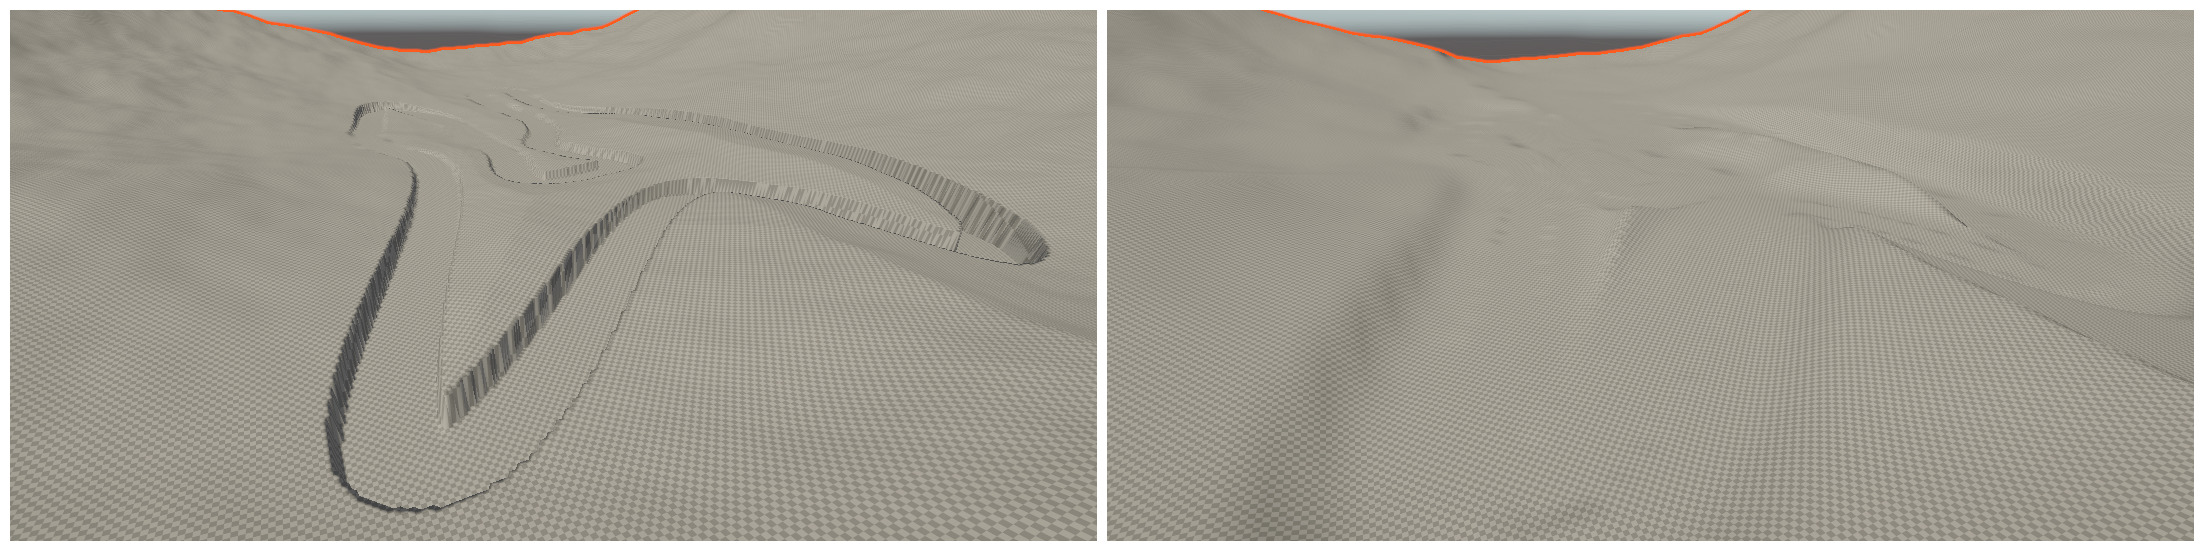
\includegraphics[width=1.0\textwidth]{img/distance_based_images/close_up_transition.jpg}
    \caption{Close-up comparison of terrain transitions. (Left) After distance-based height scaling (described in Section \ref{dbhs}), showing visible but manageable elevation differences. (Right) After enhanced distance-based smoothing, demonstrating seamless integration between fixed and generated terrain.}
    \label{fig:close_up_transition}
\end{figure}


\begin{figure}[h!]
    \centering
    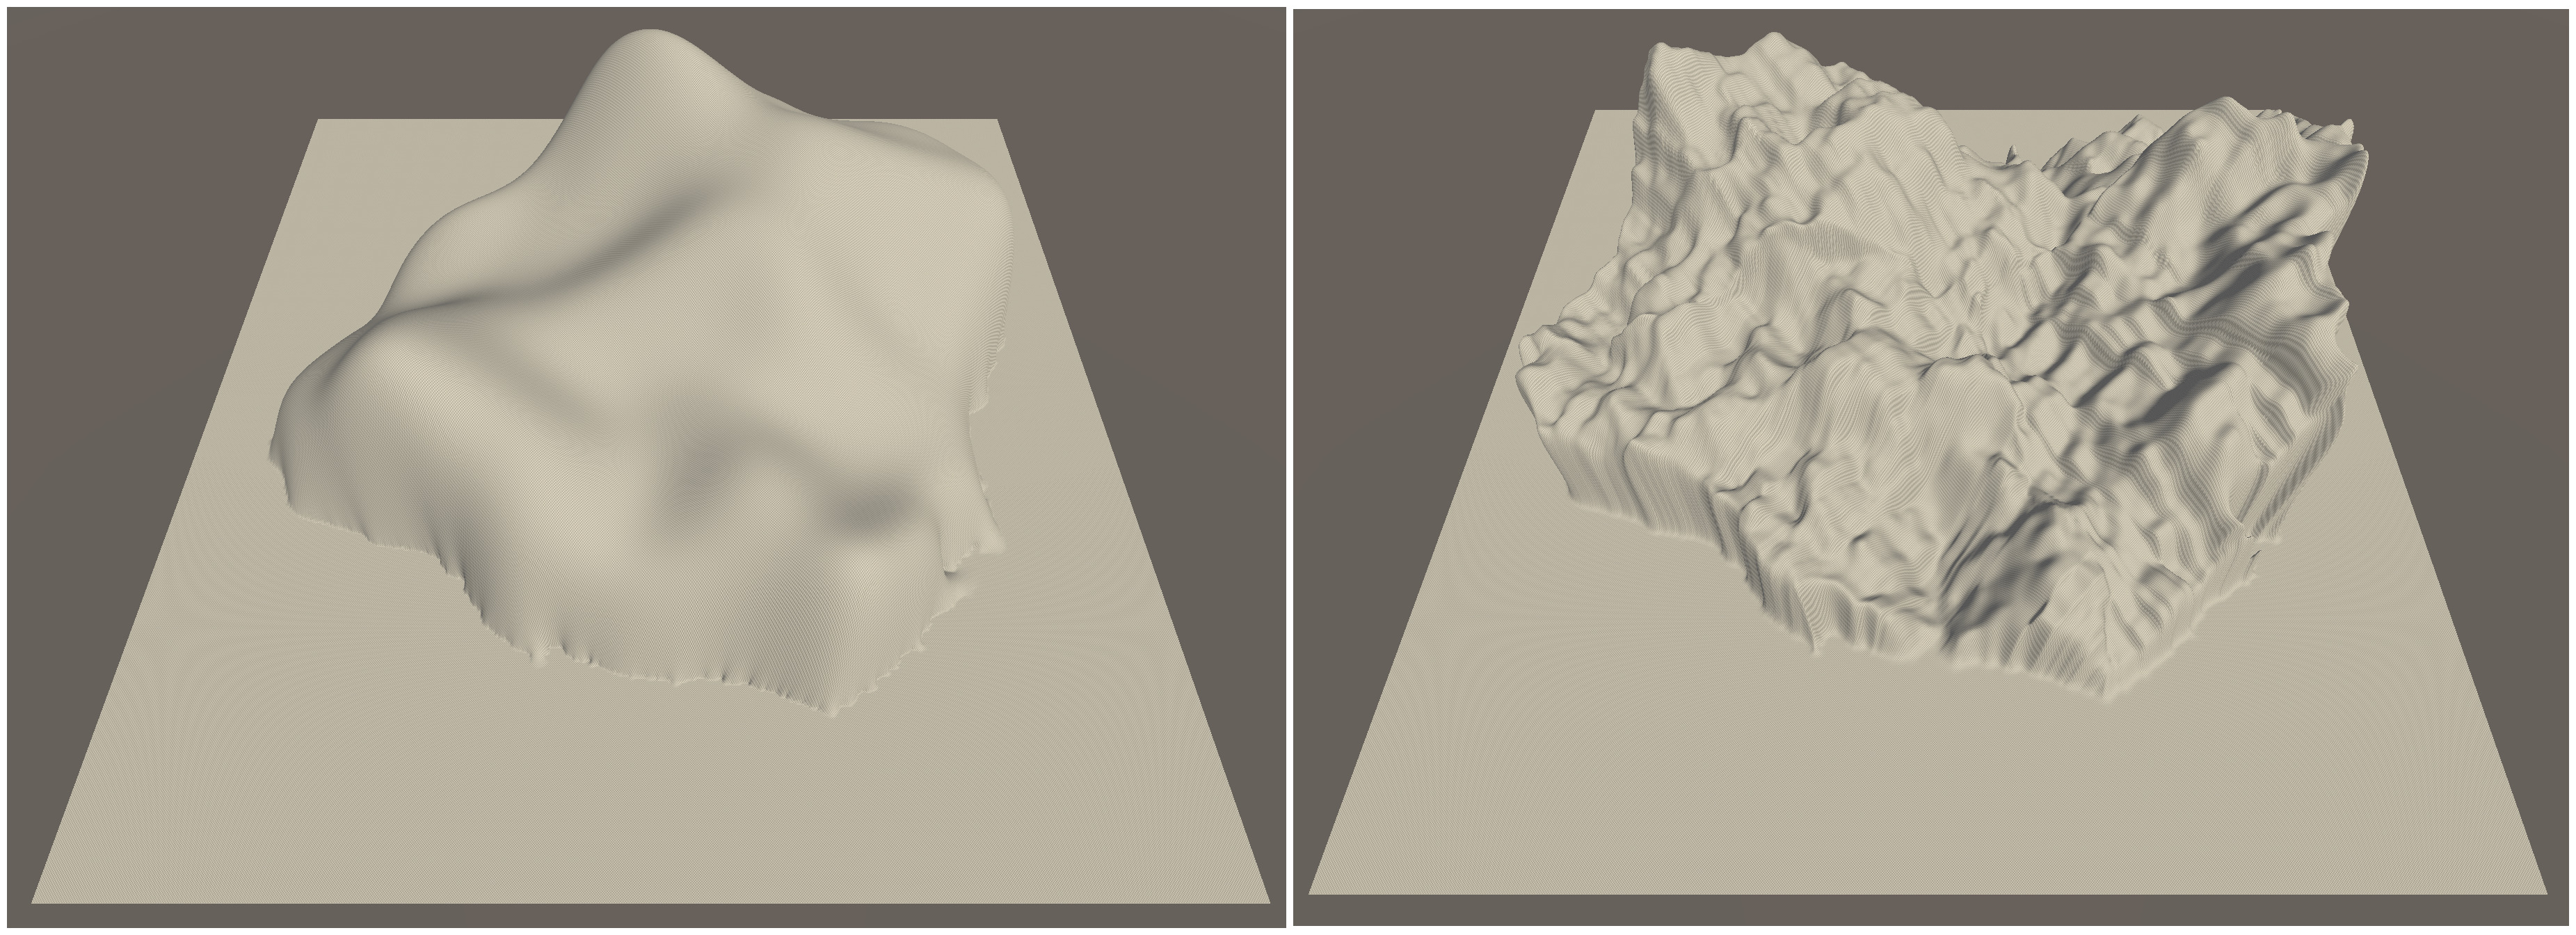
\includegraphics[width=1.0\textwidth]{img/distance_based_images/smoothing_comparison.jpg}
    \caption{Comparison of smoothing approaches on an island mask: (left) uniform smoothing loses terrain detail globally; (right) our enhanced distance-based smoothing preserves detail while creating more gentle transitions.}
    \label{fig:smoothing_comparison}
\end{figure}

\section{Distance-Based Height Scaling}
\label{dbhs}

While smoothing addresses local transitions by blending neighbouring heights, significant elevation disparities between fixed and generated areas require a fundamentally different approach. Our \textbf{distance-based height scaling} technique operates globally, adjusting the overall elevation profile of the terrain. Unlike smoothing, which preserves relative height differences while creating gradual transitions, height scaling actively modifies elevations to reduce the disparity between procedurally generated terrain and fixed constraints. 

This technique gradually adjusts terrain elevations by blending between the original procedural heights and a \textbf{reference height} -- a target elevation calculated from the fixed points' heights. The result is a terrain that naturally ``flows'' toward the constrained areas, creating realistic slopes and preventing the cliff-like formations that would otherwise appear at boundaries. The strength of how much it blends the original height towards the reference height is based on the distance to the nearest fixed point. This means that areas nearer to constraints will be closer in height to the reference height, and areas further away will maintain more of their procedurally generated height. 

Before explaining the relevant information and formal, mathematical formulation of distance-based height scaling, we present Figure \ref{fig:dbhs_effect} below to show the effects of this technique:

\begin{figure}[h!]
    \centering
    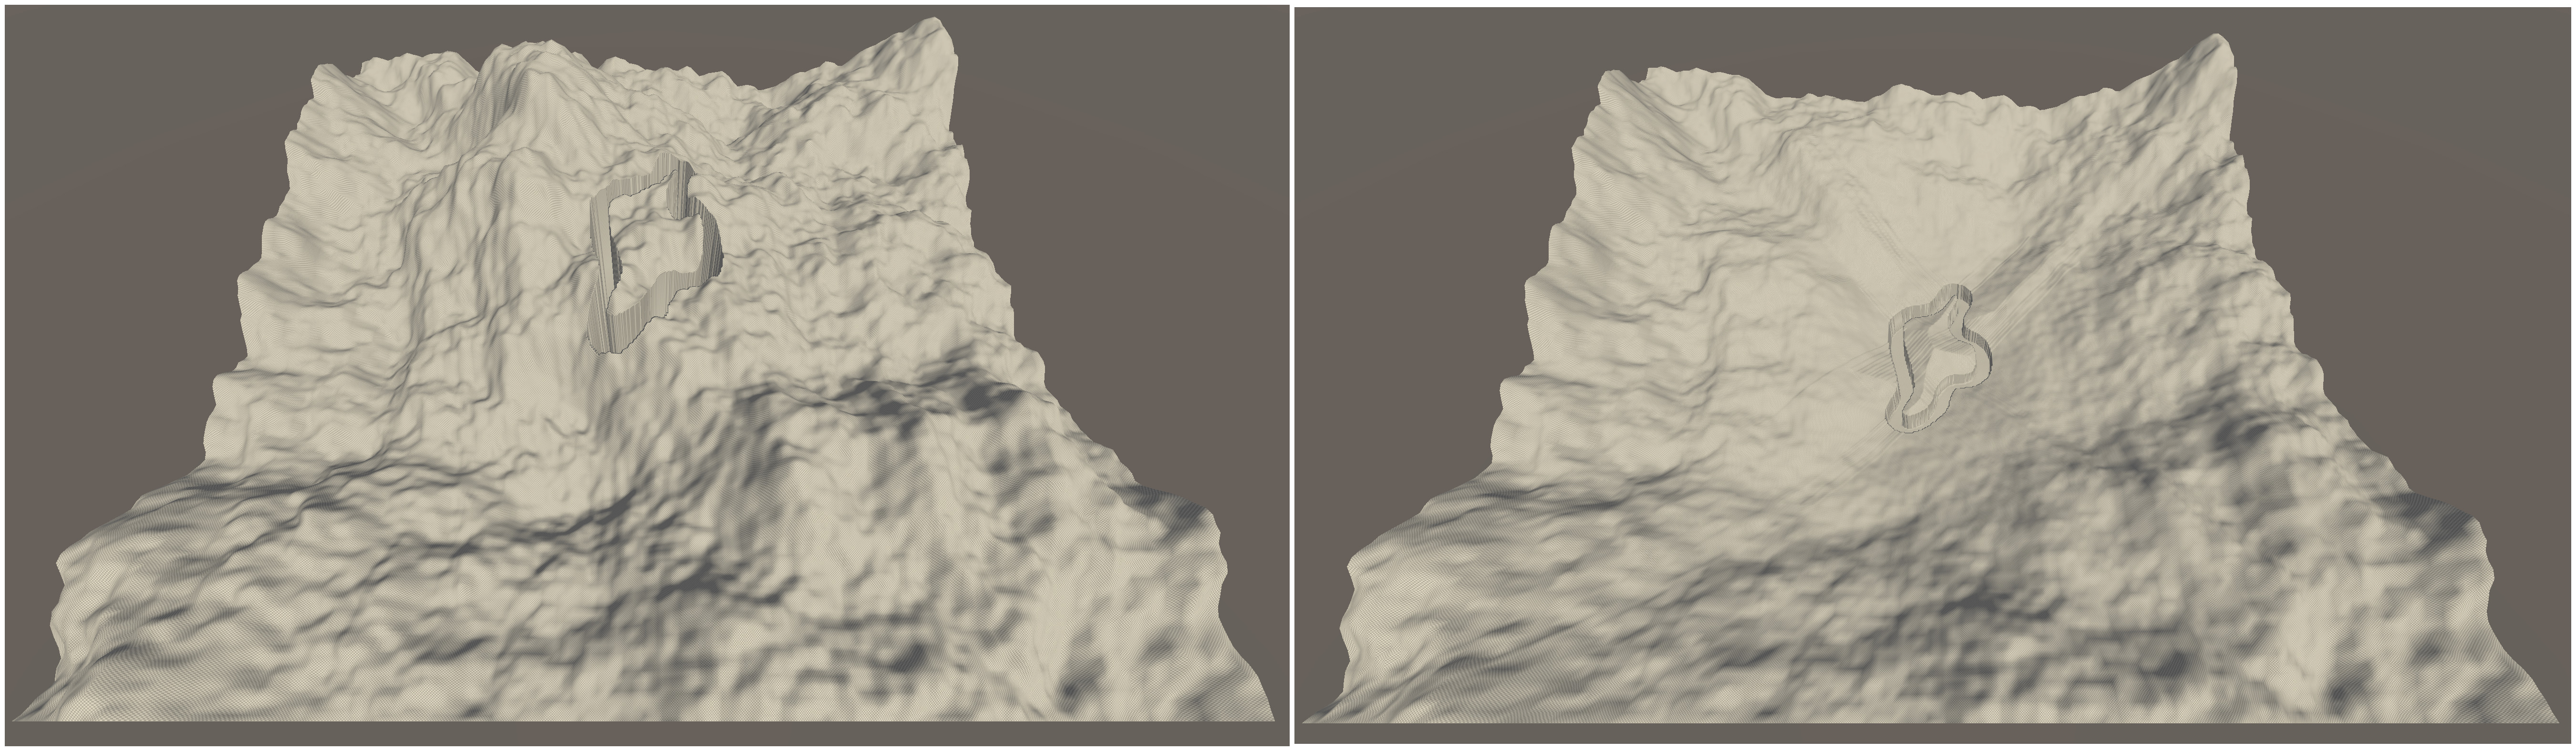
\includegraphics[width=1.0\textwidth]{img/distance_based_images/dbhs_effect.jpg}
    \caption{Distance-based height scaling effect: (Left) Perlin noise applied without any modifications to blend into the constraint, where the constraint in the middle of the terrain has abrupt transition to the surrounding area. (Right) After height scaling, showing reduced elevation disparities constraint and how the terrain now flows towards the heights of the constrained areas.}
    \label{fig:dbhs_effect}
\end{figure}

\subsubsection{Reference Height Selection}
\label{ref_height_selection}

The effectiveness of height scaling depends critically on choosing an appropriate reference height, as this is the target elevation toward which the terrain transitions. We calculate this reference height from the existing fixed points using one of three methods:

\begin{itemize}
    \item \textbf{Average Height} (default): Calculates the mean elevation of all fixed points, creating balanced transitions that work well for most constraints.
    
    \item \textbf{Minimum Height}: Uses the lowest elevation among fixed points, causing surrounding terrain to descend toward this level. 
    
    \item \textbf{Maximum Height}: Uses the highest elevation among fixed points, elevating surrounding terrain to create plateaus or mountain ranges around constrained peaks.
\end{itemize}

The choice of reference height method is not about correctness but about achieving the desired terrain characteristics. As demonstrated in Figures~\ref{fig:dbhs_base} and \ref{fig:dbhs_reference_heights}, each method produces distinctly different but \textit{equally} \textit{valid} terrain formations. The flexibility to choose between these methods allows artists and designers to achieve their specific vision while maintaining natural transitions.

\subsubsection{Mathematical Formulation}
Now we propose the mathematical approaches to this technique. The algorithm blends between original procedural heights, set by a traditional procedural terrain generation algorithm, and a reference height derived from fixed area heights. This can be formally represented as:

\[ h'(x, y) = h(x, y) \cdot s(d) + h_{ref} \cdot (1 - s(d)) \]

This equation performs a distance-weighted calculation where:

\begin{itemize}
    \item $h'(x,y)$ is the final scaled height at position $(x,y)$;
    \item $h(x,y)$ is the original procedural height at that position;
    \item  $h_{ref}$ is the \textbf{reference height} calculated from fixed points;
    \item $s(d)$ is the distance-based \textbf{scaling function} that controls the blend between original and reference heights:
    
    \[ s(d) = s_{min} + (1 - s_{min}) \cdot d_{norm} \]
\end{itemize}


The scaling function $s(d)$ creates a smooth transition, with $s_{norm}$ being the same as described in Section \ref{edbs_math}:
\begin{itemize}
    \item At fixed boundaries ($d_{norm} = 0$): $s(0) = s_{min}$, giving maximum influence to the reference height;
    \item At maximum distance ($d_{norm} = 1$): $s(1) = 1$, preserving the original procedural height
    \item $s_{min} \in [0, 1]$ controls the strength of the effect:
        \begin{itemize}
            \item $s_{min} = 0$: Complete flattening to reference height at boundaries;
            \item $s_{min} = 0.5$: 50\% blend between original and reference at boundaries;
            \item $s_{min} = 1$: No effect (original heights preserved everywhere).
        \end{itemize}
\end{itemize}

The final height calculation can be rewritten to show the blending more clearly:

\begin{equation}
h'(x, y) = \underbrace{h(x, y) \cdot s(d)}_{\text{scaled original}} + 
           \underbrace{h_{ref} \cdot (1 - s(d))}_{\text{reference contribution}}
\end{equation}

This mechanism can be rewritten as the following pseudocode:

\begin{algorithm}[H]
\small
\caption{Distance-Based Height Scaling}
\label{alg:height_scaling}
\begin{algorithmic}[1]
\Require $\text{heightMap}[w \times h]$, $\text{distanceGrid}[w \times h]$, $\text{params}$
\Ensure Height-scaled terrain with natural transitions to fixed areas

\State $h_{\text{ref}} \gets \text{calculateReference}(\text{heightMap}, \text{params.method})$
\State $\text{maxDistance} \gets \max(\text{distanceGrid})$

\For{each modifiable point $(x,y)$}
    \State $d_{\text{norm}} \gets \text{distanceGrid}[x,y] / \text{maxDistance}$
    
    \Comment{Scale factor increases with distance from fixed points}
    \State $s \gets \text{params.minScale} + (1 - \text{params.minScale}) \times d_{\text{norm}}$
    
    \Comment{Apply scaling to original height}
    \State $h_{\text{scaled}} \gets \text{heightMap}[x,y] \times s$
    
    \Comment{Calculate blend factor for reference height influence}
    \State $\text{blendFactor} \gets (1 - d_{\text{norm}}) \times (1 - s)$
    
    \Comment{Interpolate between scaled height and reference height}
    \State $\text{heightMap}[x,y] \gets \text{lerp}(h_{\text{scaled}}, h_{\text{ref}}, \text{blendFactor})$
\EndFor

\Function{lerp}{$a, b, t$}
    \State \Return $a \times (1 - t) + b \times t$
\EndFunction
\end{algorithmic}
\end{algorithm}

\textbf{Complexity Analysis}: The algorithm achieves excellent efficiency with $O(n)$ time complexity, processing each pixel exactly once. The reference height calculation adds an initial $O(n)$ scan of fixed points, and finding the maximum distance requires another $O(n)$ pass, but these are one-time costs. 

Figure~\ref{fig:dbhs_base} and \ref{fig:dbhs_reference_heights} demonstrate the visual impact of height scaling and how the different reference methods affect this.

\begin{figure}[h!]
    \centering
    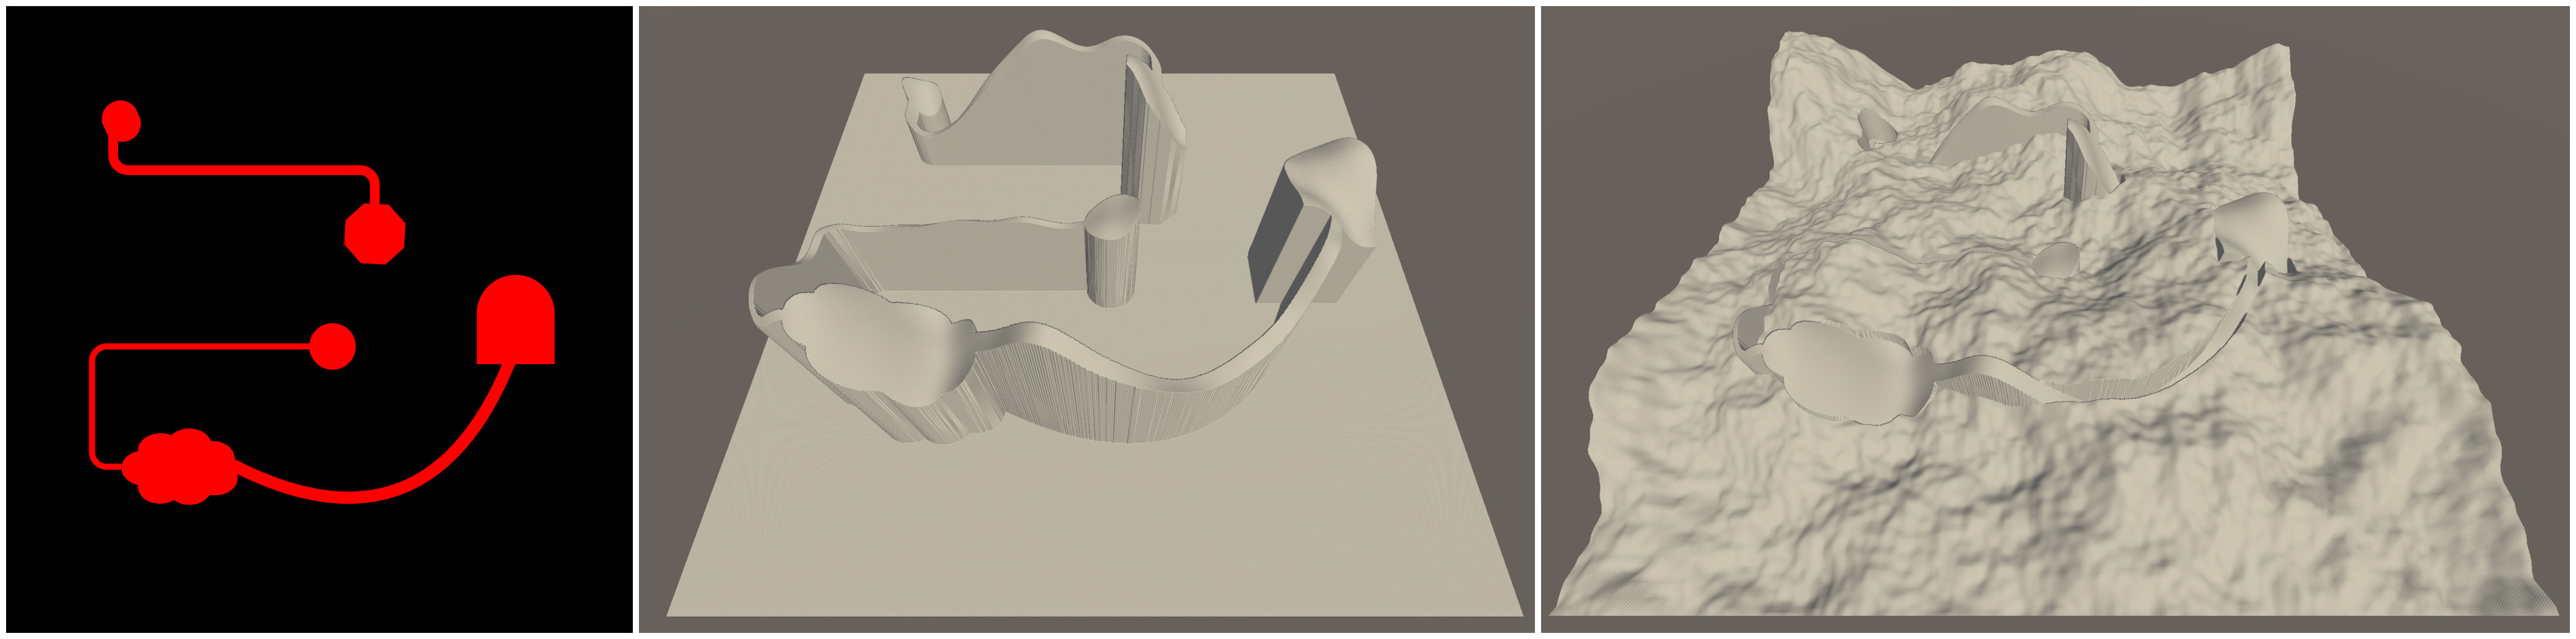
\includegraphics[width=1.0\textwidth]{img/distance_based_images/dbhs_base.jpg}
    \caption{Test terrain for demonstrating reference height methods: (Left) mask texture. (Middle) base terrain heights set in constrained areas. (Right) Perlin noise applied with no post-processing.}
    \label{fig:dbhs_base}
\end{figure}

\begin{figure}[h!]
    \centering
    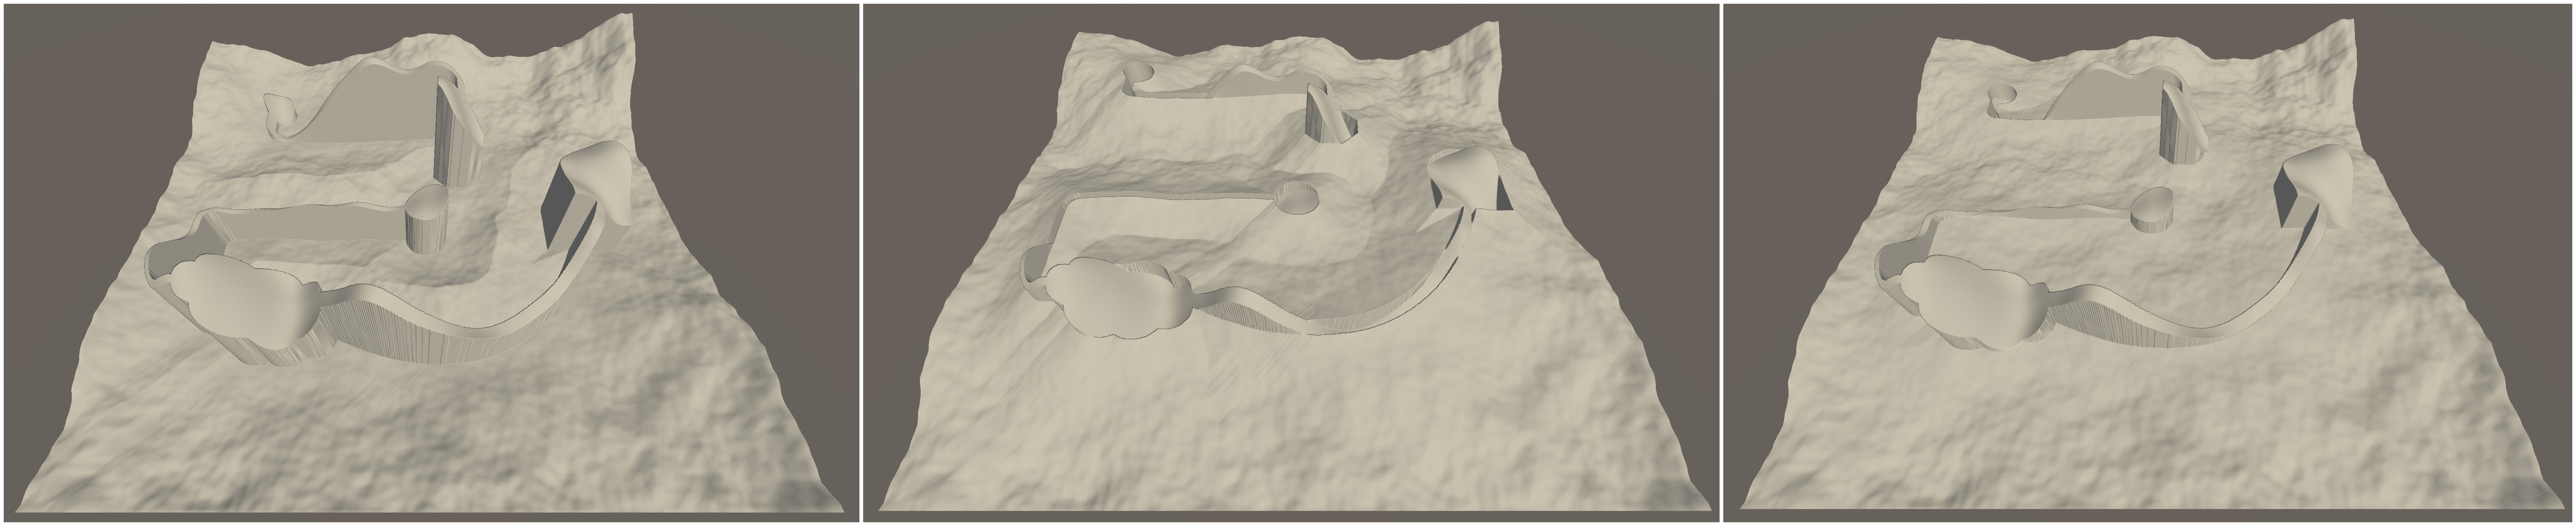
\includegraphics[width=1.0\textwidth]{img/distance_based_images/dbhs_reference_height.jpg}
    \caption{Effect of different reference heights when applying distance-based height scaling, applied to the example seen in Fig. \ref{fig:dbhs_base}. (Left) Minimum reference height used, creates valleys towards the minimum height of the constrained area. (Middle) Maximum reference height forms elevated regions around the constrained areas. (Right) Average of all constrained points as a reference height produces balanced transitions towards the mean height of the pixels in the constrained areas.}
    \label{fig:dbhs_reference_heights}
\end{figure}

\section{Summary}

This chapter presented our novel distance-based approach for creating natural transitions in constrained procedural terrain generation. By using distance from fixed points as a unifying metric, we achieve:

\begin{itemize}
    \item \textbf{Seamless integration}: Natural transitions that eliminate the boundary problem;
    \item \textbf{Algorithm independence}: Compatibility with any terrain generation technique;
    \item \textbf{Computational efficiency}: Linear $O(n)$ complexity for core operations with optional iteration-based smoothing;
    \item \textbf{Intuitive control}: Parameters with clear visual meaning.
\end{itemize}

The combination of distance-based height scaling and enhanced smoothing provides a complete solution, where height scaling addresses large-scale elevation disparities while distance-based smoothing refines local transitions without removing detail in distant areas. This two-stage approach produces terrain that appears naturally formed around fixed elements rather than artificially constrained.

Crucially, the computational efficiency of our algorithms, with single-pass $O(n)$ operations and GPU acceleration, enables the real-time feedback necessary for the Interactive Genetic Algorithm presented in Chapter~\ref{Chapter4}. Without this efficiency, the iterative parameter exploration that makes our system accessible to non-experts would be impractical. 
\chapter{Interactive Genetic Algorithm for Parameter Optimisation}
\label{Chapter4}

Building upon our distance-based approach for natural terrain transitions presented in Chapter \ref{Chapter3}, we now address the parameter optimisation challenge detailed in Section \ref{parameter_optimization}. As established in Section \ref{parameter_space_challenge}, the complexity of parameter tuning in procedural terrain generation creates significant barriers to practical adoption, particularly when multiple algorithms are combined in complex pipelines.

In this chapter, we present our specific implementation of an Interactive Genetic Algorithm (IGA) for parameter optimisation and ordering of terrain operations in constrained terrain generation. Drawing directly from the foundational work of \textcite{Walsh10} discussed in Section \ref{interactive_genetic_algorithms}, we have adapted and extended their approach to address the unique challenges of our constrained terrain generation system. Our implementation transforms parameter tuning from a technical optimisation problem into an intuitive process of guided aesthetic selection, making advanced terrain generation accessible to both technical and non-technical users.

\section{Adaptation of IGA for Constrained Terrain Generation}

Interactive Genetic Algorithms provide a powerful framework for navigating complex parameter spaces through human-guided evolution. However, applying IGA to constrained terrain generation presents unique challenges that require careful adaptation of the basic IGA framework.

The fundamental challenge lies in the intersection of two complex problem domains: the inherent parameter space complexity of procedural terrain generation and the additional constraints introduced by our distance-based approach for handling fixed height areas. This intersection creates a parameter optimisation problem that is both computationally demanding and aesthetically nuanced.

\subsection{Parameter Space Complexity in Our System}

The parameter space complexity problem becomes particularly acute in our constrained terrain generation system. Our pipeline combines multiple algorithmic components, each with its own parameter set, that must work harmoniously to produce natural-looking terrain around fixed constraints. Unlike simpler terrain generation systems that might rely on a single algorithm with a handful of parameters, our approach requires managing multiple interdependent operations.

In our specific implementation, a typical terrain might include operations such as Perlin noise generation (frequency, octaves, persistence, amplitude), Voronoi-based mountain generation (peak count, falloff rate, height ranges), distance-based smoothing operations (iteration counts, strength parameters), and erosion simulations (threshold values, erosion rates). The interdependency between these parameters, combined with the additional complexity introduced by our distance-based constraint handling, creates a parameter space that resists systematic exploration through traditional manual tuning approaches.

Consider, for example, how adjusting the amplitude of Perlin noise affects not only the overall terrain but also the effectiveness of subsequent distance-based smoothing operations. A terrain with higher amplitude variations may require more aggressive smoothing near constraint boundaries, which in turn affects the natural appearance of transitions. These parameter dependencies make manual tuning increasingly impractical as the system grows in sophistication.

\subsection{From Theory to Implementation: Addressing Previous Limitations}

Our implementation directly addresses the fundamental limitation identified by \textcite{Walsh10}: the difficulty of defining mathematical fitness functions for inherently subjective terrain quality. While their pioneering work demonstrated the feasibility of using human judgment in terrain evolution, their approach was constrained by fixed-length binary encodings that could only represent a limited parameter space.

We extend their approach in several critical ways to address the specific requirements of constrained generation and adapt it to our system. These challenges, combined with the constraint-specific modifications we introduce in our distance-based approach, make traditional parameter optimisation approaches impractical. As discussed in Section \ref{interactive_genetic_algorithms}, Interactive Genetic Algorithms provide an elegant solution by leveraging human aesthetic judgment while automating the technical aspects of parameter space exploration.

Our implementation builds directly upon the terrain generation IGA approach pioneered by \textcite{Walsh10}, but extends it in several critical ways:

\textbf{Variable-Length Genome Representation}: Unlike the fixed-length binary encoding of an individual used by \textcite{Walsh10}, our system employs flexible, operation-based individuals(genomes) that can represent varying numbers and types of terrain operations. This allows the evolution of not just parameter values but also the structure and complexity of terrain generation pipelines themselves.

\textbf{Domain-Specific Genetic Operators}: We implement specialised crossover and mutation operations designed specifically for terrain generation pipelines, incorporating domain knowledge about effective operation sequences. Rather than generic mutations, our operators understand the semantic meaning of terrain operations and can make intelligent modifications.

\textbf{Constraint-Aware Evaluation}: Our preview generation and evolution process explicitly account for fixed height constraints, ensuring that evolved solutions respect the constraint boundaries established in our distance-based approach. This integration ensures that the IGA explores only feasible solutions that can work within the constraint framework.

\subsection{Integration with Distance-Based Constraint Handling}

The integration of IGA with our distance-based constraint handling represents a key innovation in our approach. Traditional IGA implementations for terrain generation operate in unconstrained spaces where any parameter combination might theoretically produce acceptable results. Our system, however, must evolve parameter sets that work effectively within the constraints imposed by fixed height areas.

This integration manifests in several ways throughout our implementation. The genome representation explicitly includes distance-aware operations that understand constraint boundaries. The mutation operators are designed to produce variations that respect constraint requirements.

The following sections detail our specific implementation of these adaptations, demonstrating how we transform the theoretical IGA framework into a practical tool for constrained terrain generation. Through this implementation, we bridge the gap between the exploratory power of evolutionary algorithms and the precise requirements of constraint-aware terrain generation.

\section{Interactive Genetic Algorithm Design}

In this section, we provide a wide range of images of terrains relating to the interactive genetic algorithm. For consistency, we fix the same example terrain with the following mask and constraints shown in Fig. \ref{fig:iga_basis}:

\begin{figure}[h!]
    \centering
    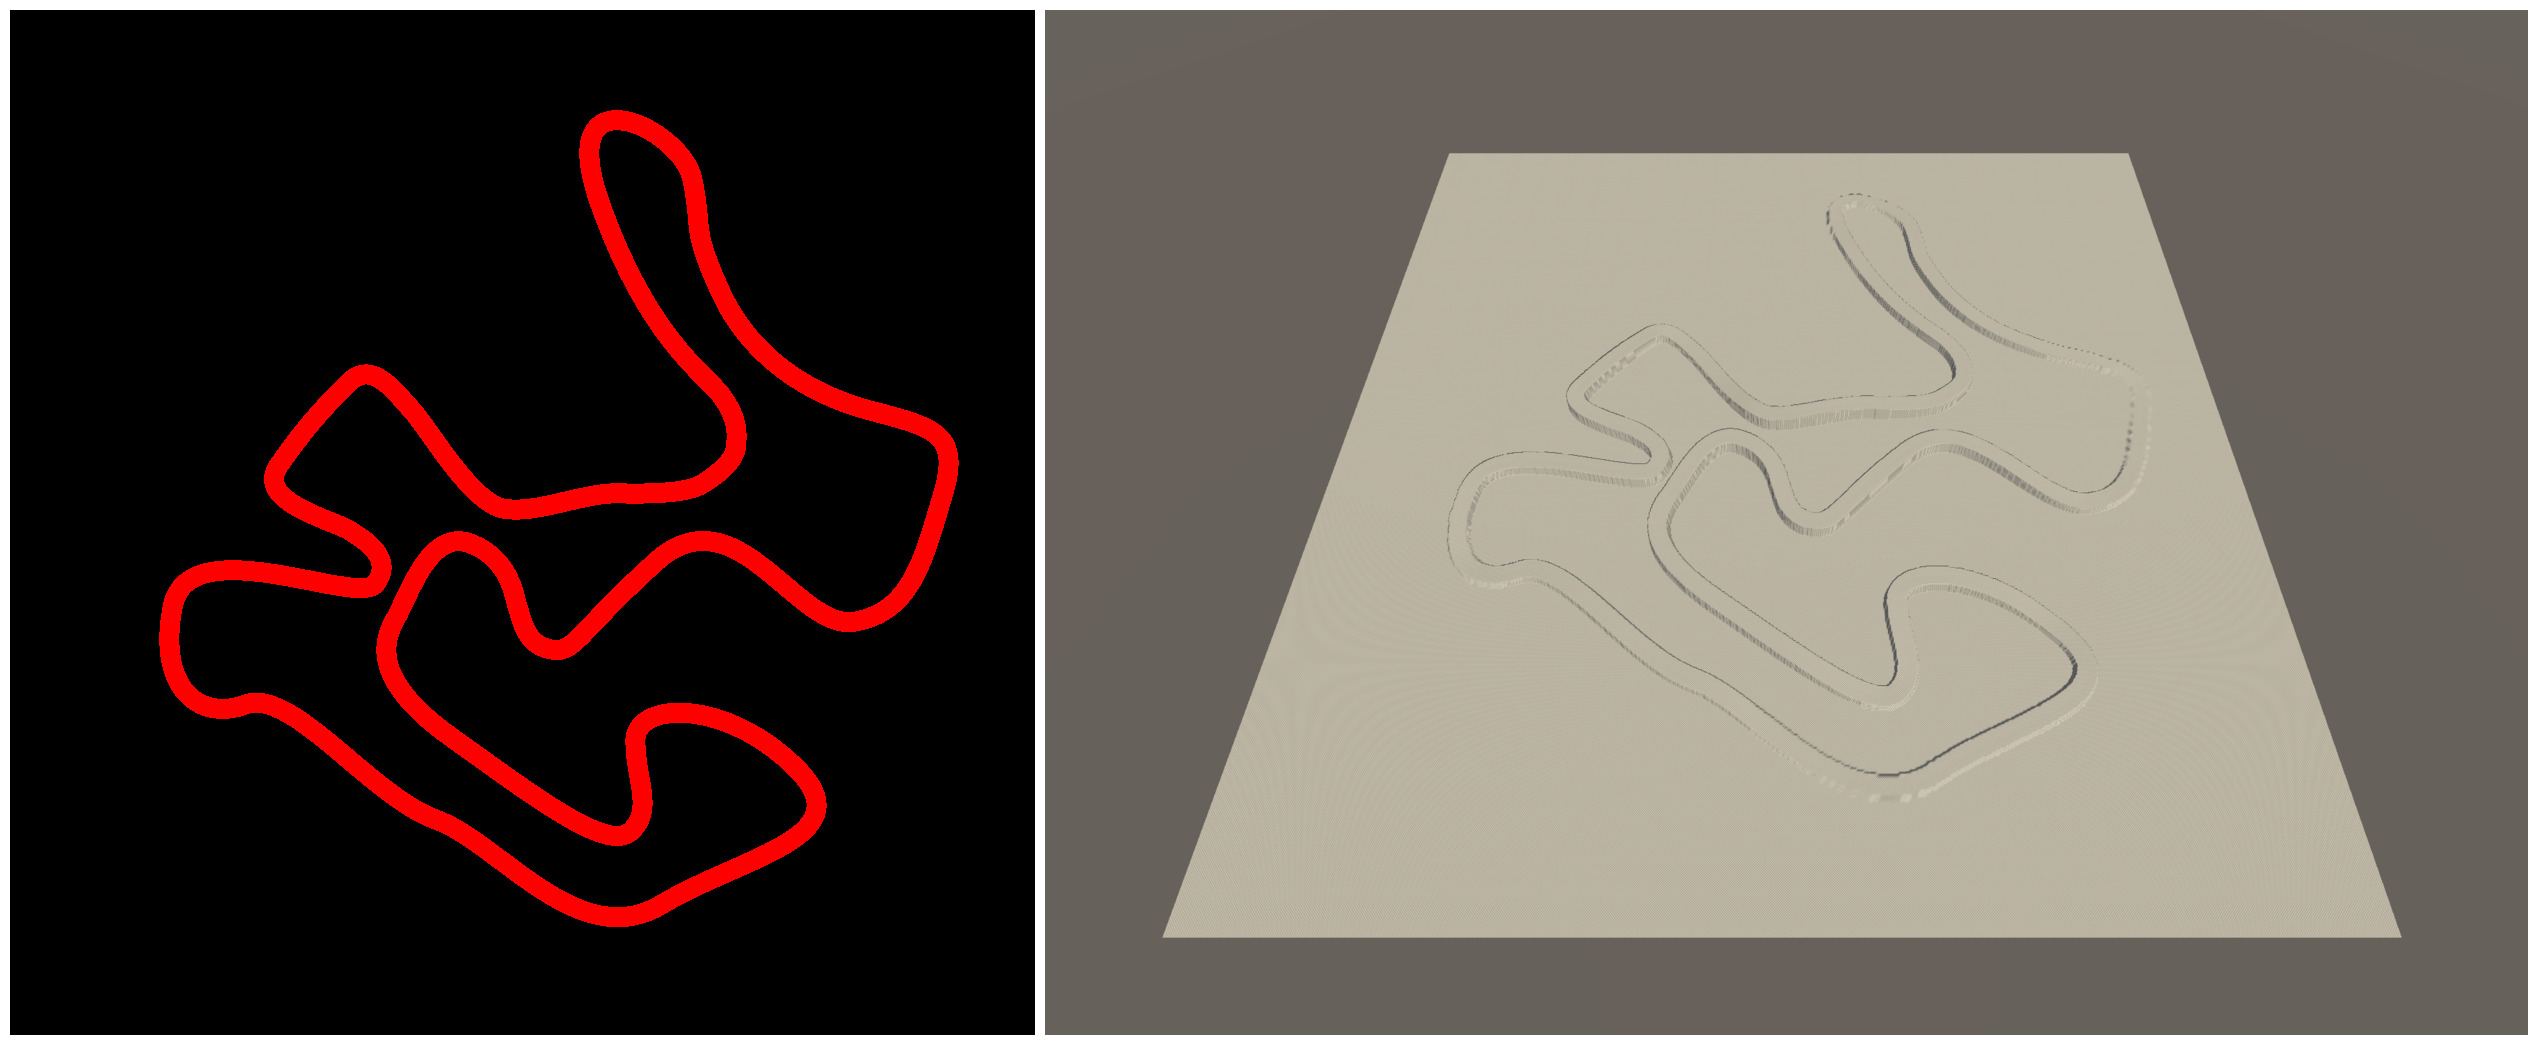
\includegraphics[width=1.0\textwidth]{img/iga_images/basis_terrain.jpg}
    \caption{(Left) constraint mask drawing, mapping non-modifiable pixels. (Right) corresponding terrain to mask with predefined heights set.}
    \label{fig:iga_basis}
\end{figure}

\subsubsection{Genome Representation}

The genome representation is a fundamental design decision that determines how candidate solutions are encoded and evolved. Unlike \textcite{Walsh10}, whose approach uses fixed-length binary strings encoding five terrain parameters, our system employs a more flexible representation that reflects the compositional nature of our terrain generation pipeline.

Each terrain \textbf{genome} in our system consists of a variable-length sequence of terrain operations, where each operation carries its own parameters. This representation offers several advantages, for example: genomes can contain different numbers and types of operations, enabling evolution of both parameters and pipeline structure. It also allows new operation types to be added without restructuring the representation. Intuitively, the genome directly corresponds to the applied operations, giving a more clear understanding of an individual candidate.

A typical genome in our system might contain operations such as:
\begin{verbatim}
Terrain Genome Operations: 
[
    VoronoiGenerator { PeakCount: 8, FallRate: 1.5, ... },
    PerlinNoiseGenerator { Frequency: 0.005, Octaves: 6, ... },
    DistanceBasedHeightScaler { MaxScaleFactor: 0.6, ... },
    EnhancedDistanceSmoother { Iterations: 40, ... },
    ThermalErosion { Iterations: 50, Threshold: 0.0015, ... }
]
\end{verbatim}

This representation captures both the operations to apply and their respective parameters, providing a rich space for evolutionary exploration.

\subsubsection{Population Initialisation and Evolution}

Our IGA system maintains a population of terrain genomes presented to users for evaluation, following the interactive evolution principles outlined in Section \ref{interactive_genetic_algorithms}. 

The initial population generation employs extensive domain knowledge to create intelligent starting points rather than purely random initialisation. Our smart initialisation system incorporates deep understanding of effective terrain generation sequences, ensuring that genomes follow natural progression patterns that respect both algorithmic dependencies and aesthetic principles.

\subsubsection{Smart Initialisation Heuristics}

Our system implements several domain-specific heuristics based on our understanding of successful terrain generation patterns:

\textbf{Operation Sequencing}: Every genome begins with a terrain generator (Perlin noise, Voronoi, or midpoint displacement) to establish base terrain features. This foundation is followed by height adjustment operations that scale terrain relative to constraint boundaries, ensuring smooth integration with fixed areas. Smoothing operations are strategically placed after major terrain modifications to create natural transitions. Finally, optional erosion and texture operations add surface detail and geological realism.

\textbf{Parameter Ranges}: Rather than using uniform random distributions, our initialisation biases parameters toward ranges that consistently produce visually appealing terrain. 

\textbf{Constraint-Aware Operations}: The system prioritises operations that work effectively with our distance-based constraint handling. Distance-based height scalers and enhanced distance smoothers appear in most genomes, as these operations directly address the boundary problem central to our approach. This ensures that evolved terrains naturally integrate with fixed height areas.

\textbf{Probabilistic Enhancement}: Certain beneficial operations are added probabilistically during initialisation. Erosion operations (50\% probability) add geological realism, while texture operations (50\% probability) provide surface detail. This probabilistic approach creates population diversity while maintaining fundamental genome quality.

This sequence demonstrates the logical progression from terrain generation through constraint integration to final refinement.

We also include a visual representation of initial individuals. For example, Figure \ref{fig:iga_initial} of our user-interface window (this is based on the terrain seen in Fig. \ref{fig:iga_basis}) shows the initial population generated. We can see the terrains are not that visually coherent in this generation, but it is a good start thanks to our heuristics, especially compared to random initialisation of operations.

\begin{figure}[ht]
    \centering
    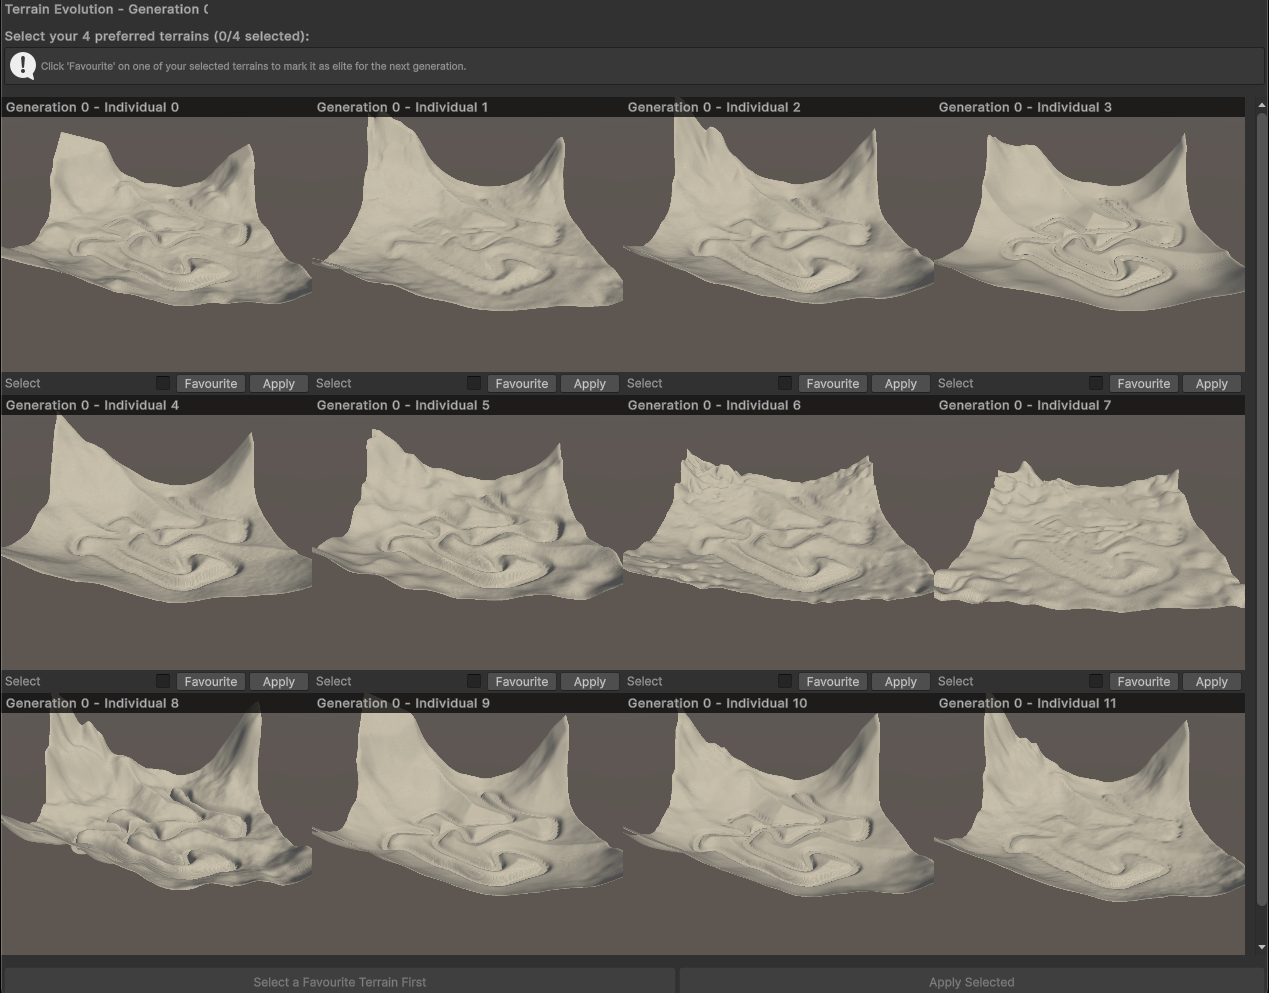
\includegraphics[width=1.0\textwidth]{img/iga_images/initial_gen.png}
    \caption{The Interactive Evolution interface showing an initial population of the terrain variants, each generated using different combinations of operations and parameters. These are all for the terrain from figure \ref{fig:iga_basis}}
    \label{fig:iga_initial}
\end{figure}

We will be using the following parameters for our example, which we chose to show a normal use case of the IGA: 

\begin{itemize}
    \item Population size -- 12;
    \item Selection count -- 4;
    \item Mutation rate -- 0.5;
    \item Crossover rate -- 0.8.
\end{itemize}

\subsubsection{Interactive Selection and Fitness Evaluation}

The selection mechanism in our IGA differs \textit{fundamentally} from traditional genetic algorithms. Rather than using a mathematical fitness function, \textbf{users} evaluate terrains \textbf{visually}, selecting those that best represent their aesthetic goals. This makes the process very subjective, as the final terrain will be heavily influenced by what the user deems a good candidate. This captures design intentions that would be difficult to encode algorithmically.

Our selection interface allows users to select multiple terrains that exhibit desirable characteristics, mark one terrain as a "favourite" for \textbf{elitist preservation}, apply any terrain directly to see it at full resolution, and continue evolution. The multi-selection approach provides rich feedback, allowing users to indicate different appealing aspects across multiple terrains.

This process is demonstrated in Figure \ref{fig:iga_selection} below, representing the selection interface window of our application:

\begin{figure}[h!]
    \centering
    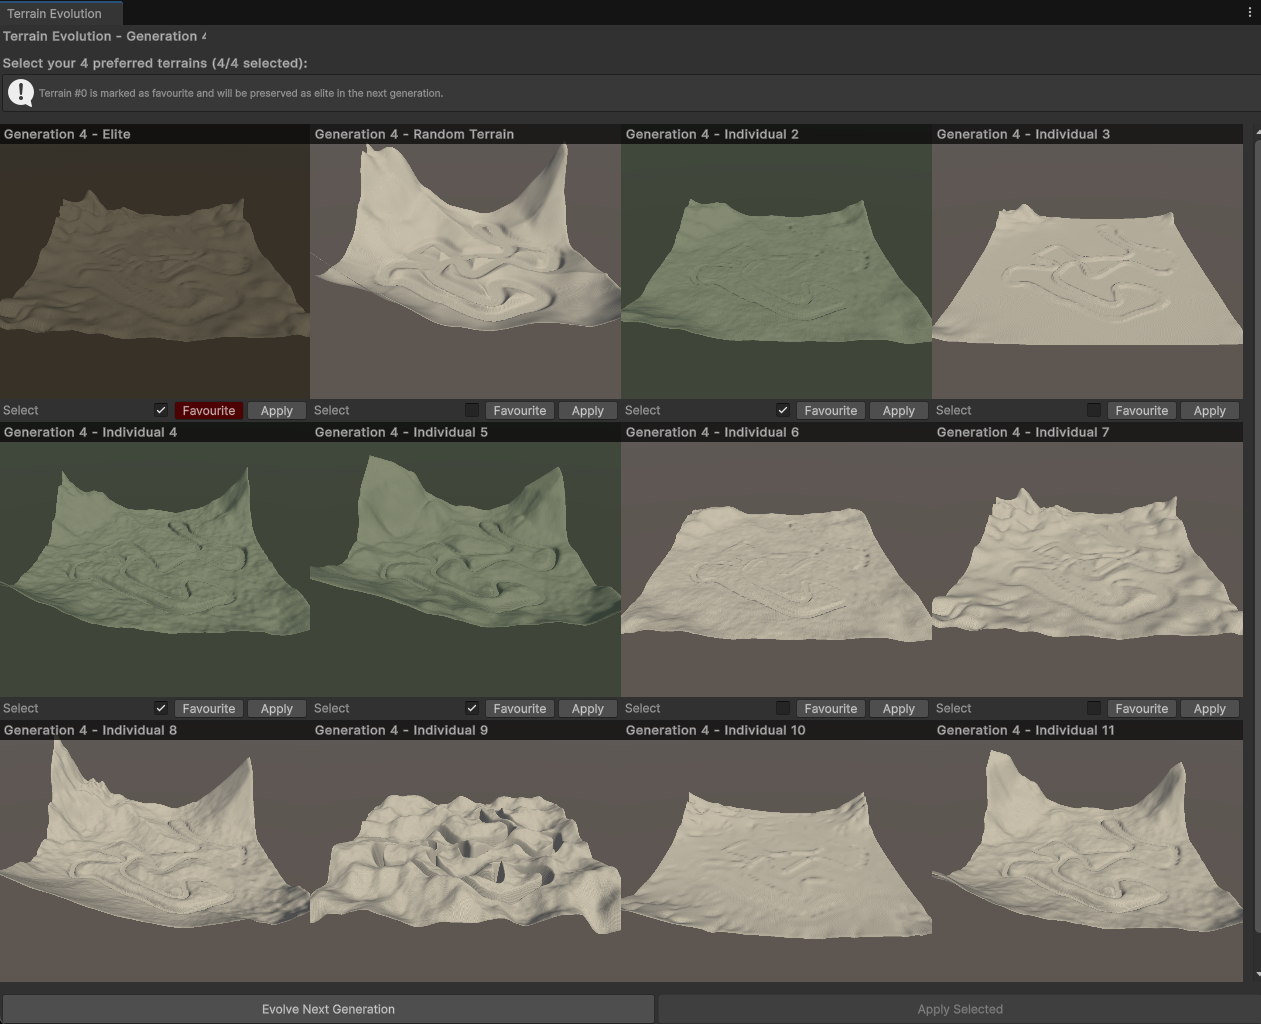
\includegraphics[width=1.0\textwidth]{img/iga_images/selection_window.png}
    \caption{The selection interface showing four selected terrains (green) with one marked as favourite (red) for elitist preservation in the next generation. This is the result after four generations.}
    \label{fig:iga_selection}
\end{figure}

The inclusion of an explicit ``favourite'' mechanism implements elitism, ensuring the best solution from the user's perspective is preserved across generations. This addresses a common problem in genetic algorithms where promising solutions can be lost through genetic operations.

\subsubsection{Genetic Operations}

Our genetic operations are adapted to work with our representation of a terrain genome.

\textbf{Crossover} operates at the operation level. Given two parent genomes, we select random crossover points in each parent, take operations before the crossover point from the first parent, and append operations after the crossover point from the second parent. 

\textbf{Mutation} Our mutation operators extend beyond random parameter modification to implement domain-aware genetic variations:
\begin{enumerate}
    \item [-] Structural Mutations: Rather than randomly altering existing operations, our system adds new operations at strategic locations. Height-scaling mutations insert multiple distance-based height scalers at different pipeline stages, creating graduated height transitions. Extreme smoothing mutations add intensive smoothing sequences to address particularly challenging constraint boundaries.
    \item [-] Texture Mutations: These operations add fine-scale detail through low-amplitude noise generators followed by appropriate smoothing. The system automatically adjusts parameters to ensure texture detail does not interfere with constraint boundaries.
    \item [-] To prevent genome bloat, removal mutations eliminate 3-6 operations randomly, allowing successful core operations to dominate the pipeline. This balances genetic diversity with computational efficiency.
\end{enumerate}

Below we present Figure \ref{fig:final_gen} that demonstrates the evolutionary progress of terrain variants over generations:

\begin{figure}[h!]
    \centering
    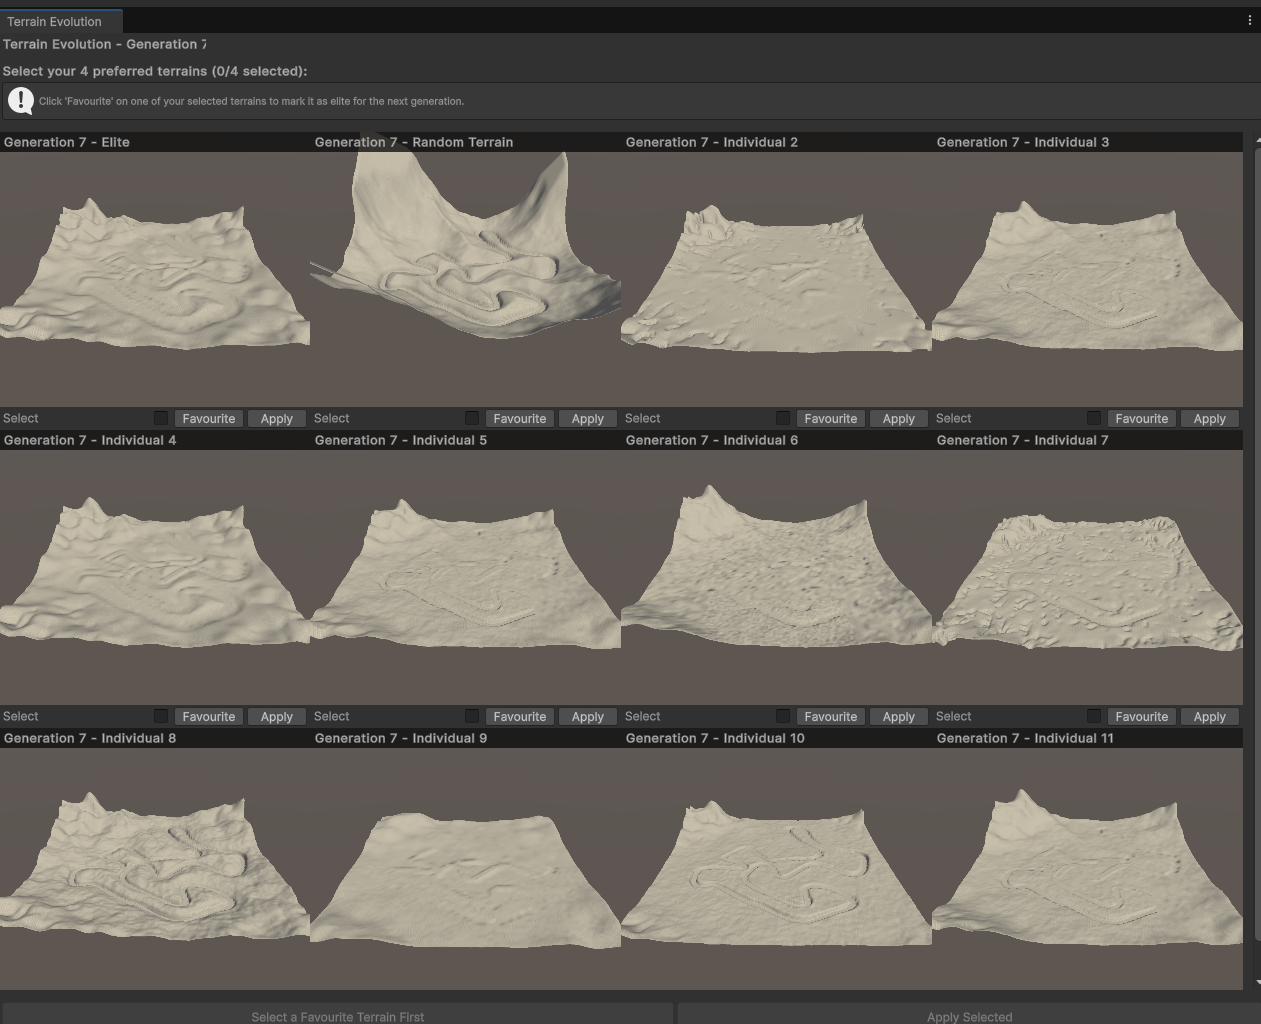
\includegraphics[width=1.0\textwidth]{img/iga_images/final_gen.png}
    \caption{Evolution progress showing terrain variants after multiple generations, demonstrating convergence toward user preferences to flatter terrains in this example, while maintaining some diversity.}
    \label{fig:final_gen}
\end{figure}

We also include Figure \ref{fig:iga_results_flat} which is the \textbf{elite} terrain taken from Fig. \ref{fig:final_gen} (top left). This demonstrates more clearly how well our IGA approach works.

\begin{figure}[h!]
    \centering
    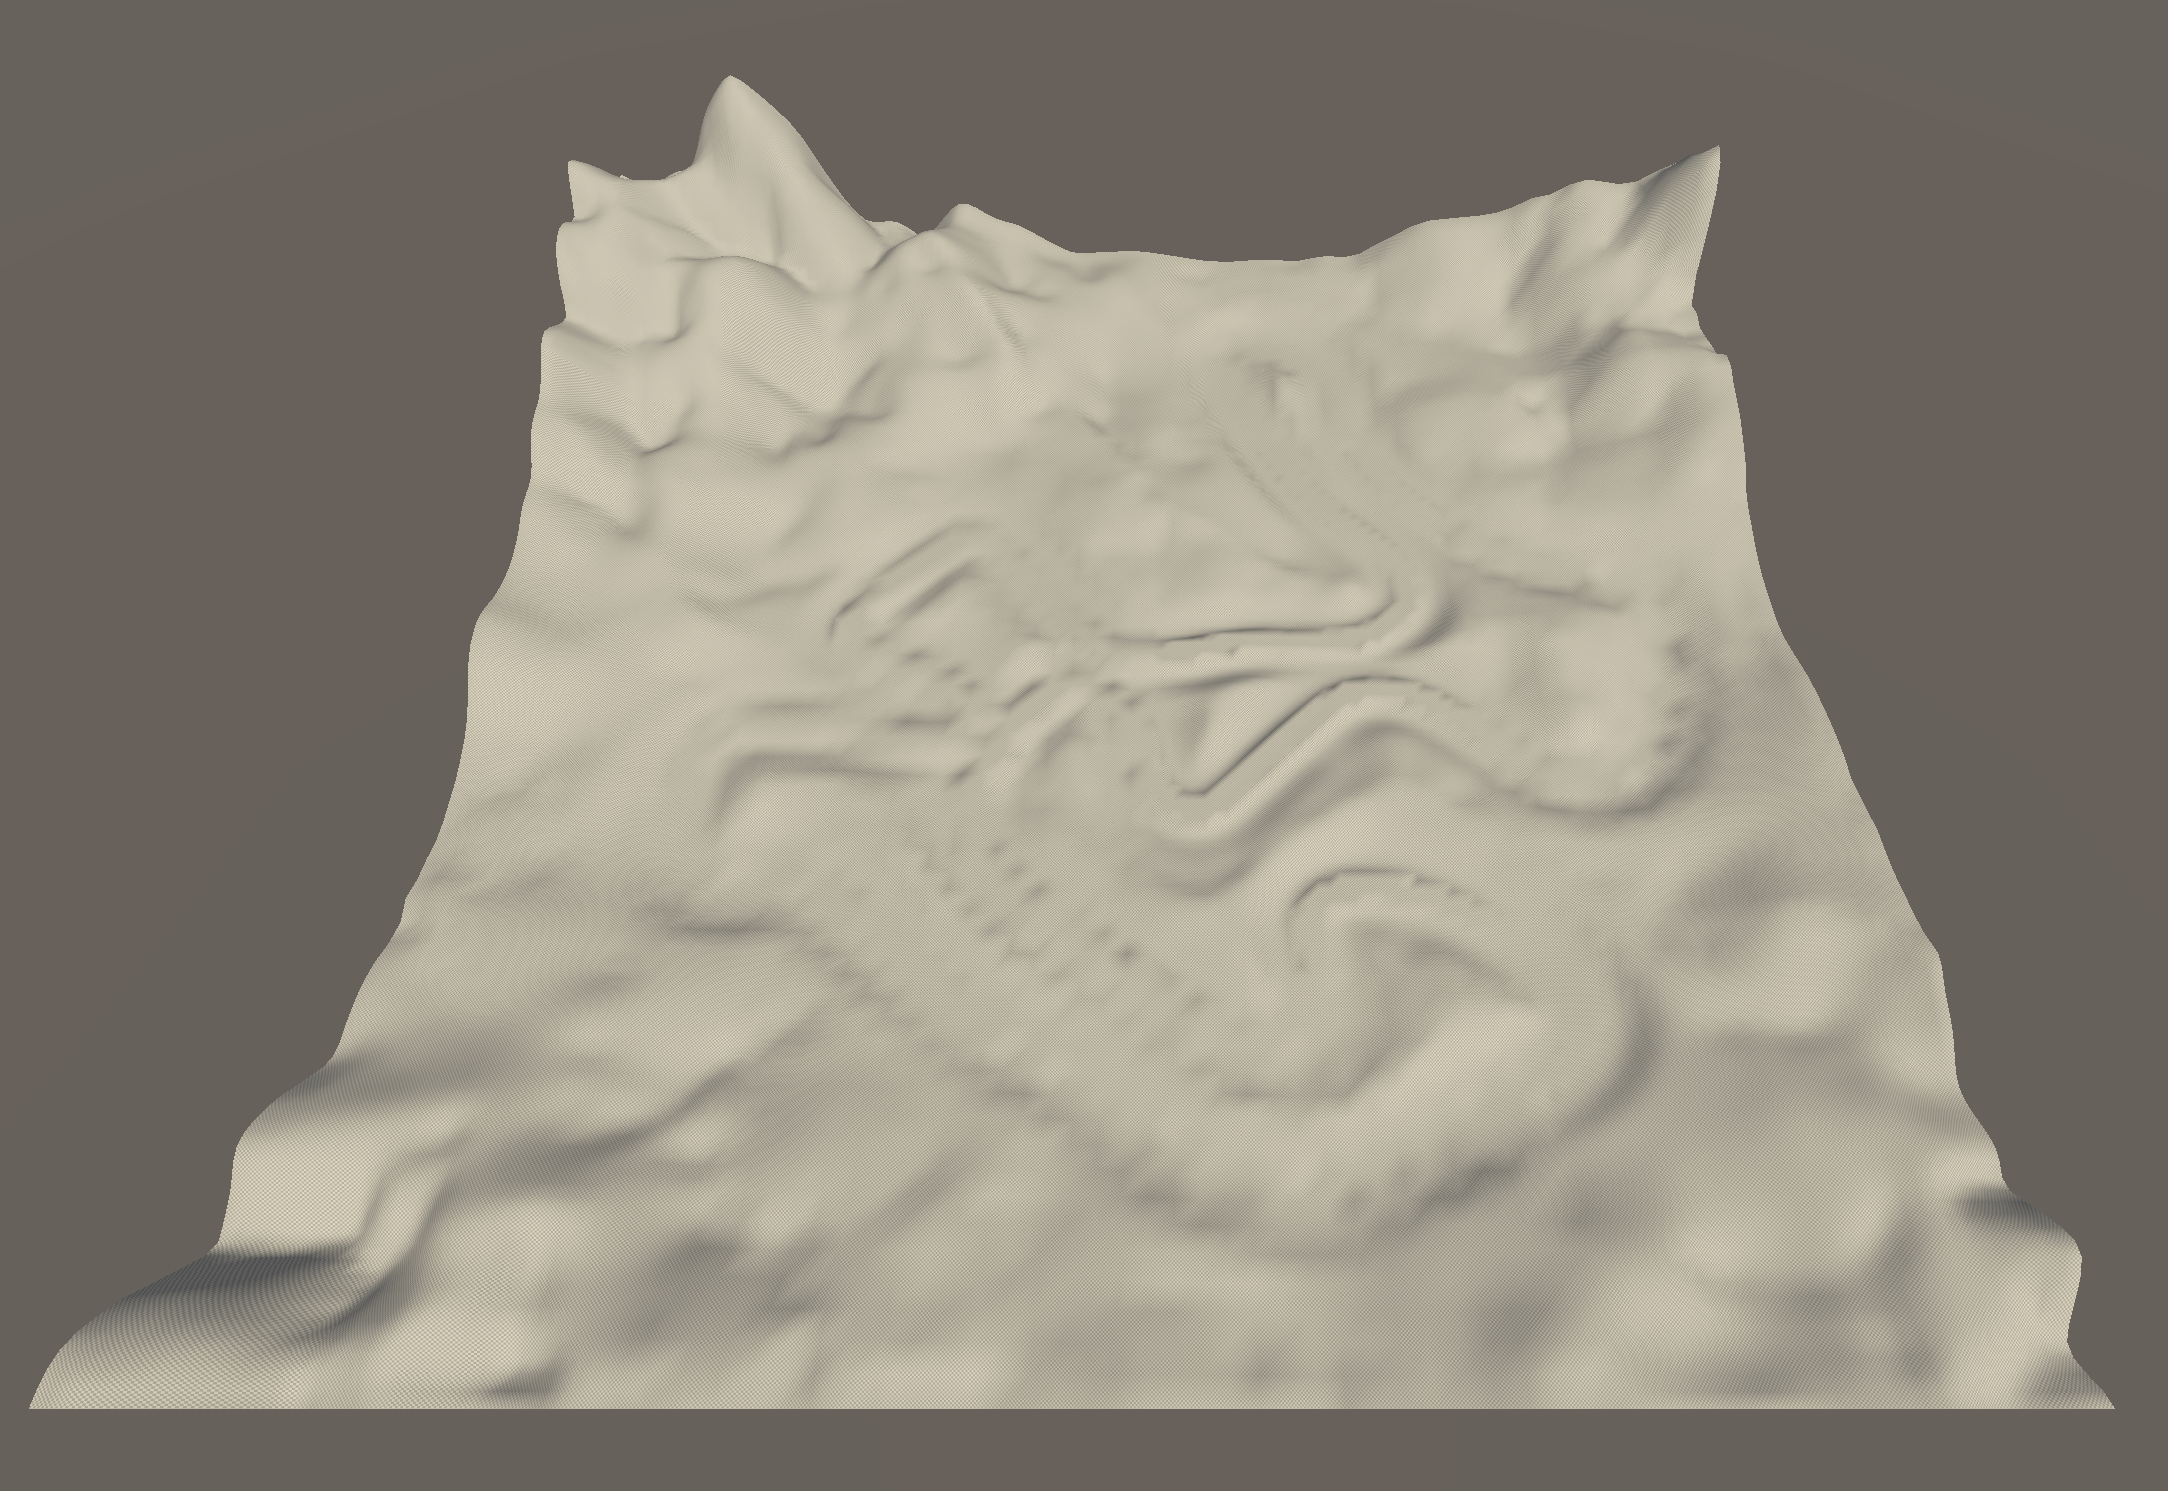
\includegraphics[width=1.0\textwidth]{img/iga_images/gen_7_result.png}
    \caption{Final terrain example from the 7th generation in the above terrain evolution window \ref{fig:final_gen}. This is the elite terrain (seen in the top left of the evolution window) applied to the actual terrain. This was fully generated using the IGA, where the user had a preference to a flat, bumpy terrain around their constraint.}
    \label{fig:iga_results_flat}
\end{figure}

\section{Implementation and User Experience}

Our IGA implementation leverages Unity's editor capabilities to provide an integrated, responsive experience. The system generates quick previews by capturing the current terrain state, applying each genome's operations, rendering from a carefully chosen camera angle, and restoring the original terrain. 

The evolution process typically converges toward satisfactory results within 5-10 generations, though users can continue evolving indefinitely to explore alternative solutions. The system's ability to discover novel parameter combinations often surprises users, producing terrain configurations they would not have considered through manual tuning.

\section{Parameter Tuning and System Configuration}
\label{parameter_tuning}

While our IGA system provides intuitive parameter exploration through human-guided evolution, the effectiveness of the evolutionary process itself depends on careful configuration of the genetic algorithm parameters. The balance between exploration and exploitation, a fundamental consideration in evolutionary algorithms discussed in Section \ref{genetic_algorithms_fundamentals}, directly influences both the quality of results and user experience.

\subsection{Core IGA Parameters}

Our system exposes four primary parameters that control the evolutionary dynamics:

\textbf{Population Size} determines the number of terrain variants presented to users in each generation. We usually use a population size of 12 - 32, as this is a good balance between efficiency and diversity. 

\textbf{Selection Count} specifies how many individuals users choose as parents for the next generation. We typically recommend selecting 25-40\% of the population (3-6 individuals). Higher selection pressure (fewer selected individuals) accelerates convergence but risks premature convergence to local optima. Lower selection pressure (more selected individuals) maintains diversity longer but may slow progress toward user preferences.

\textbf{Crossover Rate} controls the probability that two parent genomes will exchange genetic material. Our default of 0.7 balances recombination benefits with parent preservation. Higher rates (0.8-0.9) encourage exploration of new parameter combinations but may disrupt successful genome structures. Lower rates (0.4-0.6) preserve parent characteristics more strongly but reduce the algorithm's ability to discover novel solutions.

\textbf{Mutation Rate} determines how frequently random modifications occur in offspring genomes. Unlike traditional genetic algorithms that use low mutation rates (0.01-0.05), our system usually employs higher values (0.5-0.8) to compensate for small population sizes. The domain-specific nature of our mutation operators, which add terrain-appropriate operations rather than random parameter changes, allows for more aggressive mutation while maintaining genome viability.

\section{Summary}

In this chapter, we have presented our specific implementation of Interactive Genetic Algorithm techniques for parameter optimisation in constrained procedural terrain generation. Building upon the theoretical foundation established in Section \ref{interactive_genetic_algorithms} and the pioneering work of \textcite{Walsh10}, we have developed a practical system that addresses the parameter space complexity challenges detailed in Section \ref{parameter_space_challenge}.

Our key technical contributions extend beyond the basic IGA framework presented in Chapter \ref{Chapter1}: a flexible, operation-based genome representation that captures both pipeline structure and parameters; constraint-aware genetic operations designed specifically for our distance-based terrain generation approach; domain-intelligent initialisation leveraging terrain generation knowledge for quality starting populations; enhanced selection mechanisms including elitist preservation through user-designated favourites; and seamless Unity integration providing rapid visual feedback for interactive evolution.

The IGA addresses the fundamental challenge identified in Section \ref{parameter_optimization}: the formalisation of subjective terrain quality in procedural generation systems. By leveraging human judgment directly within the evolutionary framework, we create a system that naturally adapts to individual preferences and design goals while navigating the complex parameter interactions inherent in constrained terrain generation.
\chapter{Evaluation and Results}
\label{Chapter5}

Having developed our distance-based approach for constrained procedural terrain generation and the Interactive Genetic Algorithm for parameter optimisation, we now finally turn to evaluating the effectiveness of our system. This chapter presents a comprehensive assessment of our approach through visual quality analysis, performance measurements, and comparative analysis. 

\section{Evaluation Methodology}

Our evaluation methodology combines visual assessment with performance analysis to provide an understanding of the system's capabilities. We recognise that terrain quality is \textit{inherently subjective} and context-dependent, making pure quantitative metrics insufficient for capturing the nuanced aspects of ``natural'' terrain appearance. Therefore, the visual assessment is based on our subjective judgement, but we aim to be consistent and reasonable by using clear criteria as described in the following Section \ref{visual_crit}. 

\subsection{Visual Quality Assessment}
\label{visual_crit}

Defining what constitutes ``natural-looking'' terrain presents an interesting challenge in procedural generation. For our evaluation, we establish several visual criteria that guide our assessment:

\begin{itemize}
    \item \textbf{Smooth Transitions}: The terrain should exhibit seamless blending between fixed and procedurally generated areas, without visible boundaries or abrupt height changes that betray the constraint locations;
    
    \item \textbf{Geological Possibility}: Generated features should resemble formations that could exist in \textbf{nature}, avoiding mathematically perfect patterns or unrealistic configurations that immediately signal algorithmic generation;
    
    \item \textbf{Contextual Coherence}: The terrain must appear as though the fixed elements (roads, buildings, water bodies, etc.) were naturally placed within an existing landscape, rather than the landscape being artificially constructed around them. However, if the constraints are unnatural looking themselves, we cannot expect the overall terrain to look good, as we can not modify the predefined constraints, and can only do our best with the modifiable areas;
    
    \item \textbf{Feature Variety}: Natural terrain exhibits variation in both large-scale features (hills, valleys) and fine details (surface texture, erosion patterns). Our generated terrain should demonstrate similar multi-scale variety.
\end{itemize}

While we acknowledge the subjective nature of visual assessment, we aim to be reasonable and critical in our analysis of our own results. We will also compare the visual results of our solutions with previous solutions based on these criteria. 

\subsection{Performance Metrics}
\label{performance_metrics}

Instead of just evaluating visual quality, we also wanted our system to run quickly. Although the time complexity of algorithms has been discussed in previous chapter, we will also measure the actual time it takes to perform certain tasks related to using our system. All the performance evaluation focuses on practical usability within the Unity development environment. All tests were conducted on an Apple MacBook Air (2025) with Apple M4 chip and 16GB RAM, running Unity 6000.0.41f. While absolute timing values are hardware-dependent, the relative performance differences between operations and approaches remain informative. 
We decided against analysing the memory usage of our system, as our system did not have an objective to be memory efficient. Memory also does not tend to be a limiting factor for adoption of a procedural terrain generation system, and most systems related to this have similar memory usage.


\section{Test Scenarios and Case Studies}
\label{case_studies}

Our evaluation explores diverse constraint patterns that we created representing real-world use cases. Each test scenario challenges different aspects of the system, some testing how it handles connected constraints, other testing how it handles constraints with extreme height disparities. We aim to display and evaluate a variety of example case studies to show the versatility and results of our system, and we believe that the five test cases discussed in this section adequately demonstrate this. 

Since our system also allows great flexibility in the users' preference of taste, whether they desire a smooth terrain of rolling hills or a rough and eroded mountain range, the final terrain is ultimately influenced by their choices, regardless of whether they are interacting with it through the manual approach or IGA approach. We try to have a slightly different preference in our taste in each case study, depending on what we decide would look good for the specific input constraint. 

As our system can handle two approaches of generation (see section \ref{interaction_models}), we will show an example of a terrain generated using each approach: (1) the manual approach and (2) generated using the Interactive Genetic Algorithm. When evaluating the manual approach, we will not provide the details of the exact terrain operations and their respective parameters that were applied to achieve this resulting terrain. We omit this information for the sake of brevity and because this section is rather to show what is possible with our system, not the exact instructions to achieve a specific result for a given example. Note that this section focuses only on \textbf{visual quality assessment} according to the criteria established in Section \ref{visual_crit}, and \textbf{performance evaluation} will be discussed in Section \ref{performance_eval}. \footnote{For readers interested in hands-on experimentation, our Unity project (see User documentation) includes numerous pre-configured scenes with masks and terrain setups.  This allows immediate testing without the overhead of creating custom constraint configurations, lowering the barrier to exploring the system's capabilities.}

% Case Study 1
\subsection{Road/Path network constraint}

This case study aims to show our systems ability to deal with linear features at reasonably similar elevation levels, testing the system's ability to create natural landscape around roads, race tracks and paths. 
In our example, we will use the constraint combination as seen in Fig. \ref{fig:constraint_1}, with the mask texture seen on the left, and the respective predefined heights seen on the right. 

% \hfill

\begin{figure}[h]
    \centering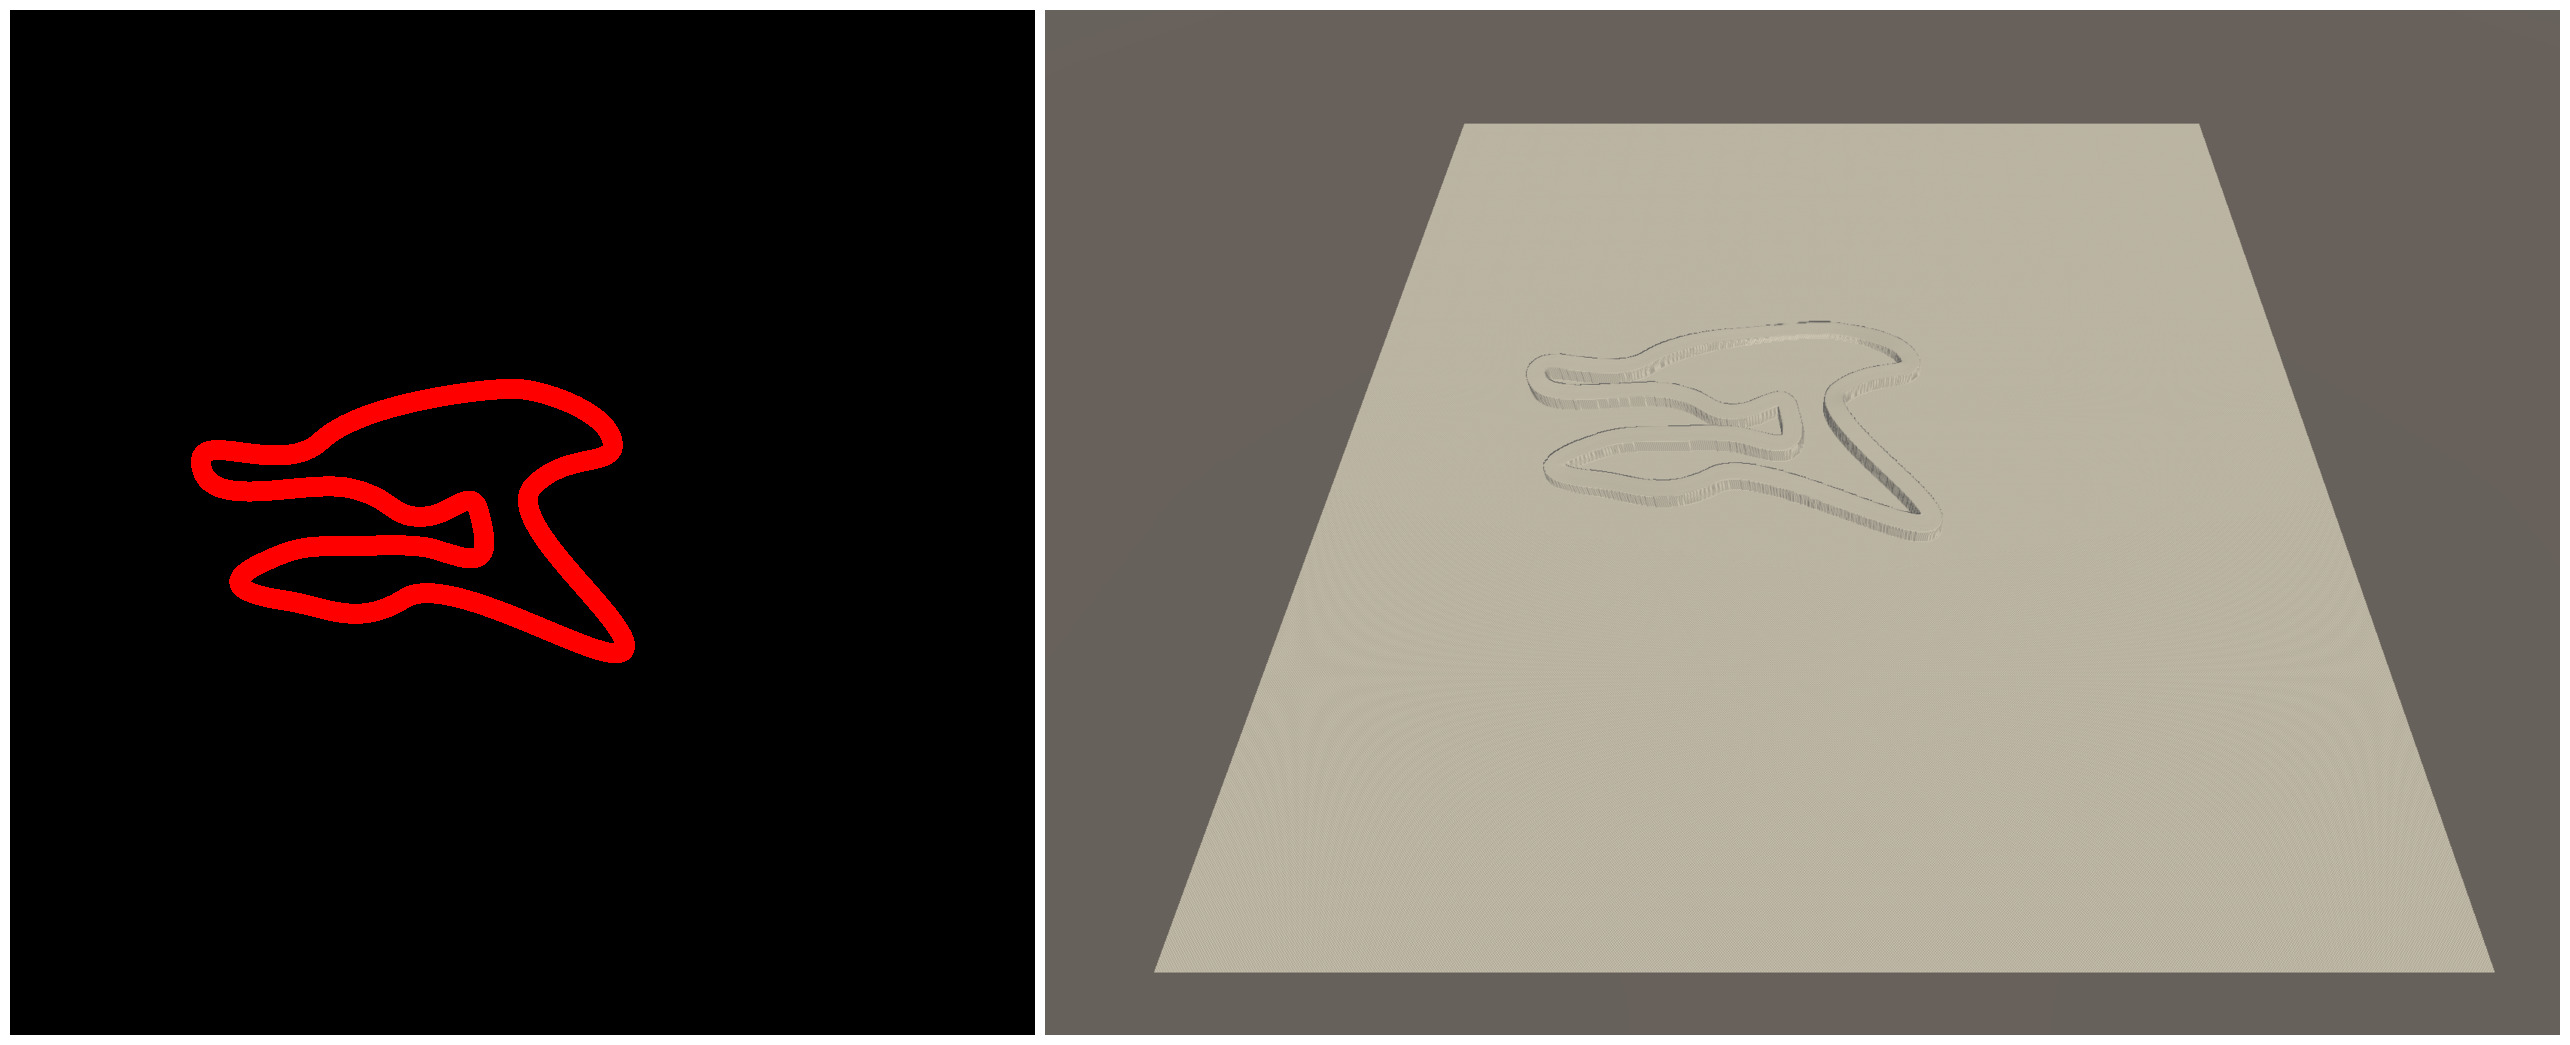
\includegraphics[width=0.65\linewidth]{img/evaluation/1/constraint_1.jpg}
    \caption{The input into our system. (Left) shows the mask texture provided. (Right) shows the set heights for the pixels mapped out by the mask texture.}
    \label{fig:constraint_1}
\end{figure}


% \hfill

\textbf{Manual Approach:} In Figure \ref{fig:manual_image_1}, we can see an example of a terrain generated using the manual interaction approach.

\begin{figure}[h]
    \centering
    \includegraphics[width=0.6\linewidth]{img/evaluation/1/manual_image_1.png}
    \caption{Resulting terrain of \ref{fig:constraint_1} generated using manually set terrain operations.}
    \label{fig:manual_image_1}
\end{figure}


% \hfill

% \hfill


\textbf{IGA Approach:} In Figure \ref{fig:iga_image_1}, we can see an example of a terrain generated using the IGA approach.

\begin{figure}[H]
    \centering
    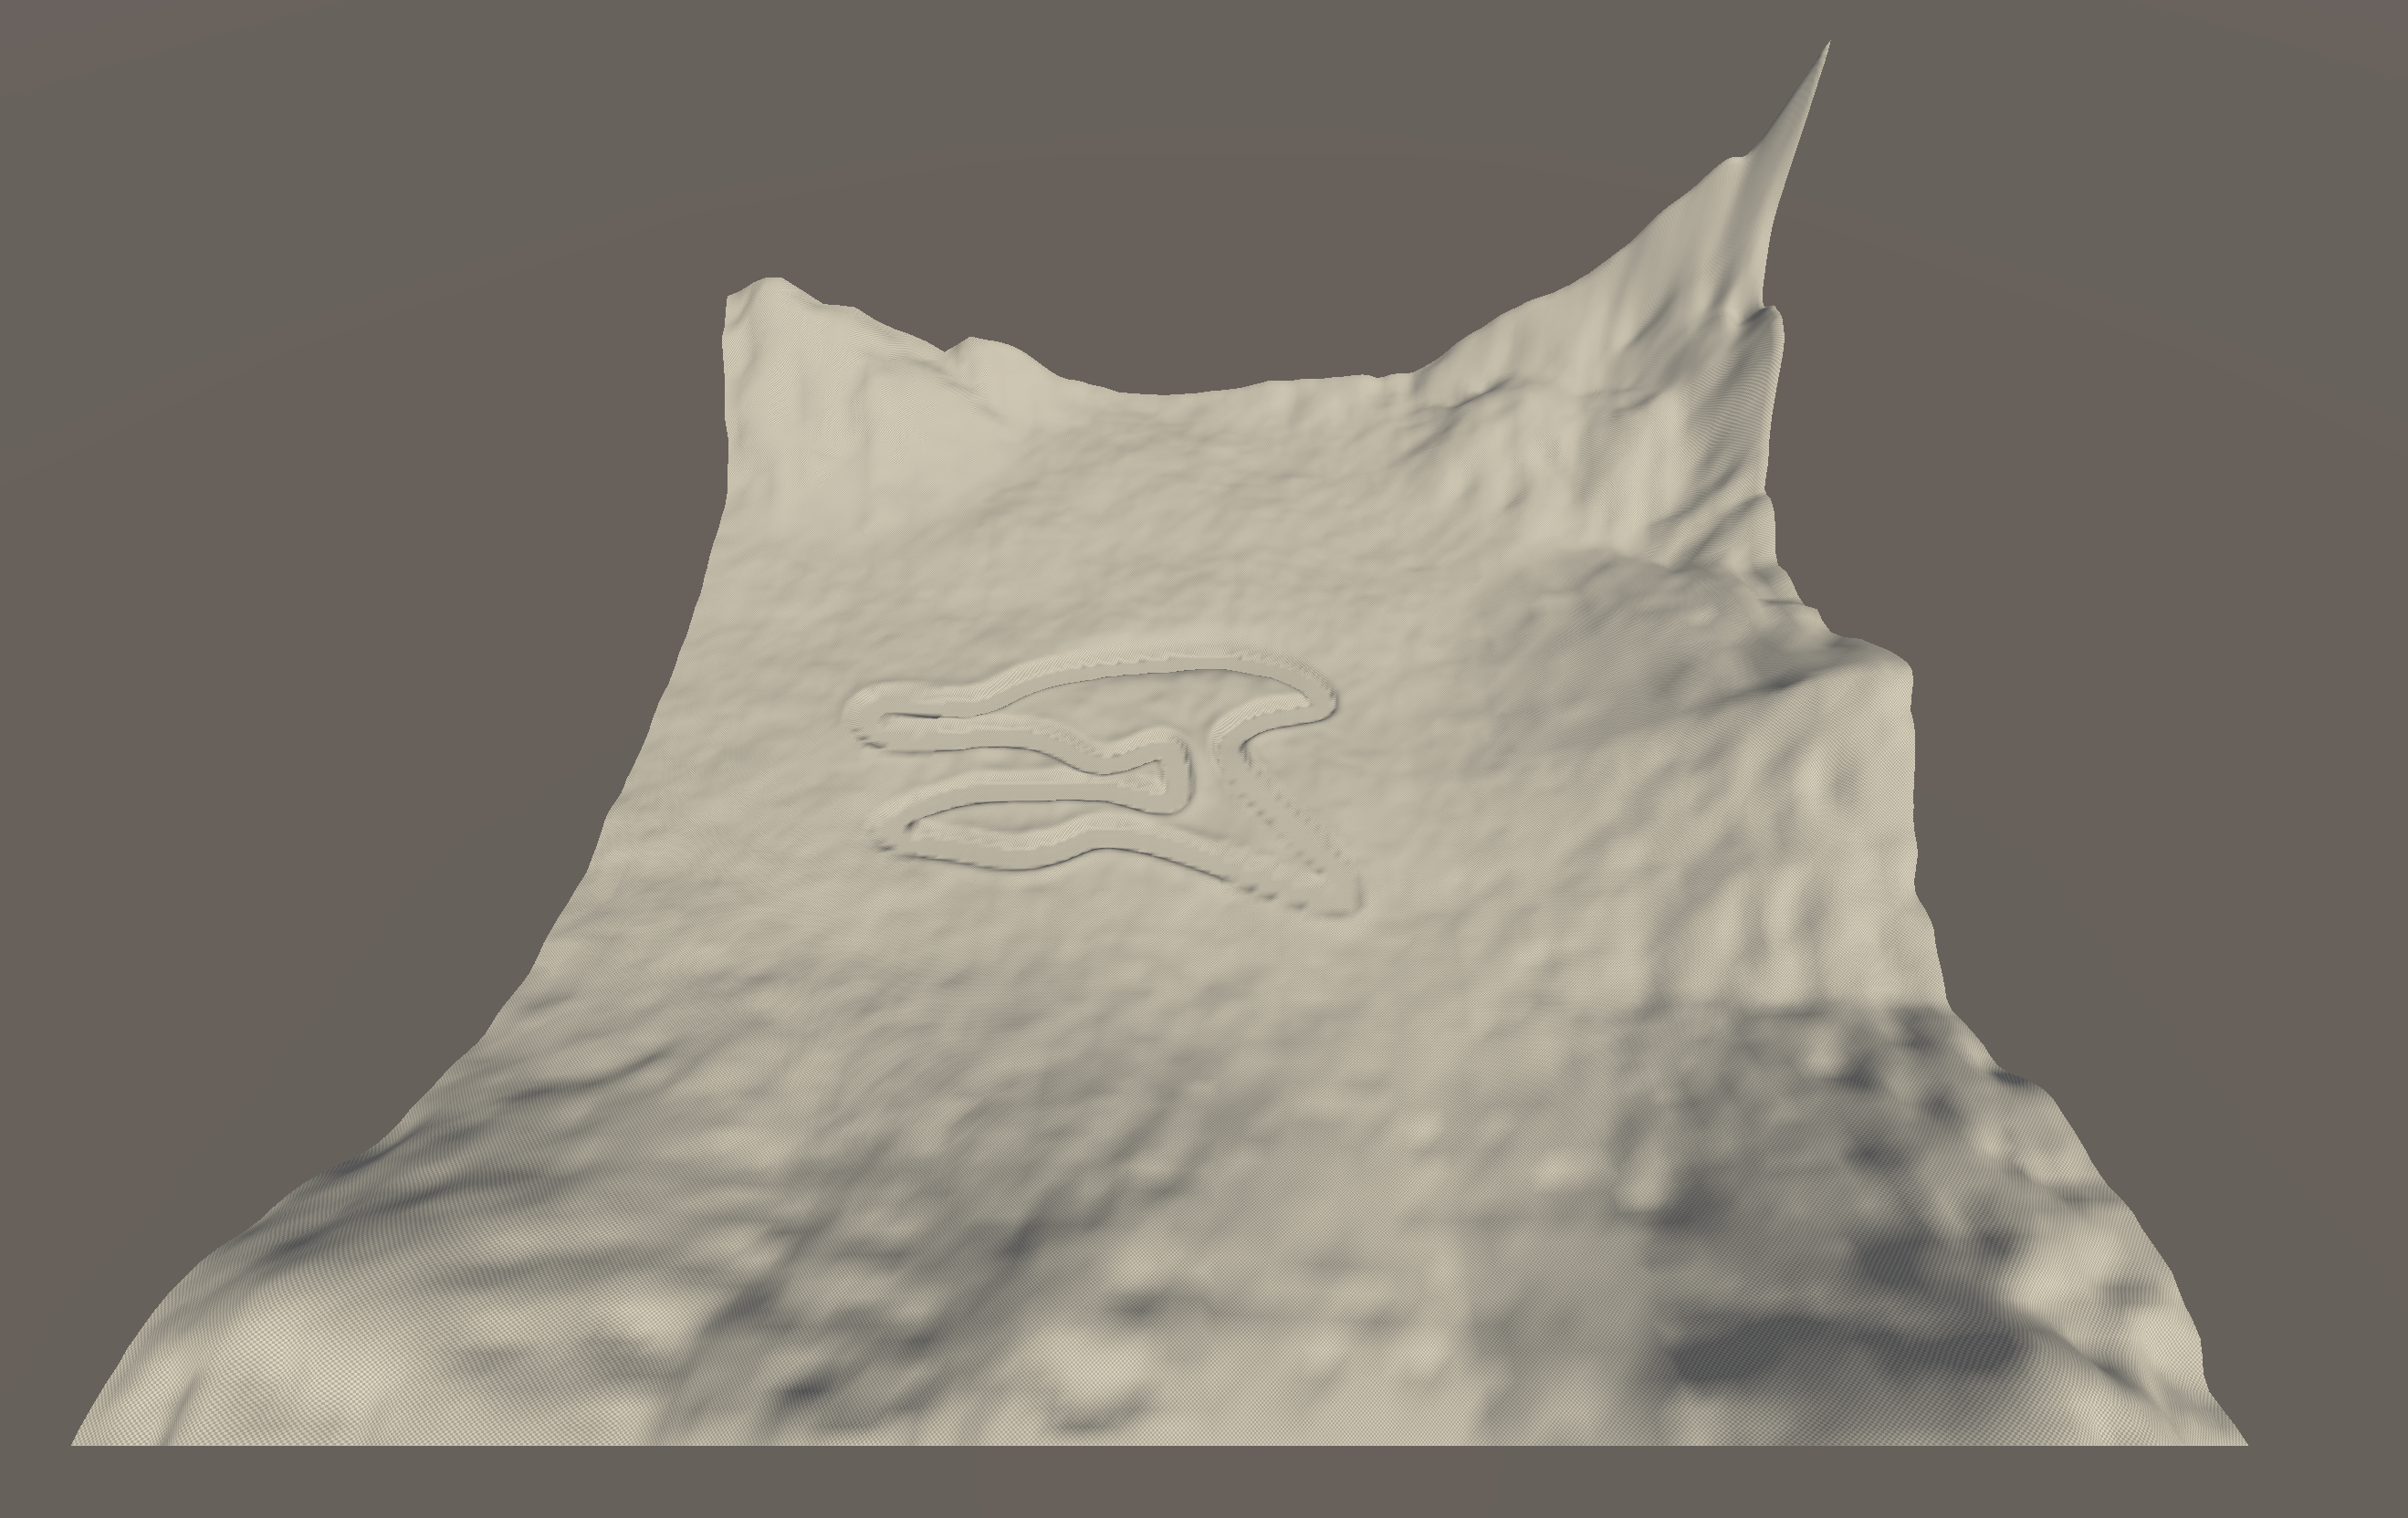
\includegraphics[width=0.6\linewidth]{img/evaluation/1/iga_image_1.png}
    \caption{Resulting terrain of \ref{fig:constraint_1} generated using the IGA evolution window.}
    \label{fig:iga_image_1}
\end{figure}


% Case Study 2
\subsection{Foundations constraint}
In this specific use case, it is important to note that our system has the objective to blend the surrounding terrain into the fixed areas, so we will not be testing or evaluating examples that would not normally have this in the real world (e.g. houses, trees or objects). This thesis focuses on only the procedural terrain generation of the heightmap, not on object placement.

However, if a developer is using our system, and they want to effectively place objects on top of the terrain in specific areas at given heights, we recommend they (1) draw this foundation, (2) generate the terrain, and (3) then place the objects on top of the terrain as they please. 

This way, the foundations on which the objects are placed will blend naturally into the surrounding terrain, and the objects they place will sit on top of these at the desired location and height.

Here we aim to show our system's ability to deal with disconnected foundation blocks placed around the terrain, each with a different uniform height. We will use the constraint combination as seen in Figure \ref{fig:constraint_2}: 

\begin{figure}[H]
    \centering
    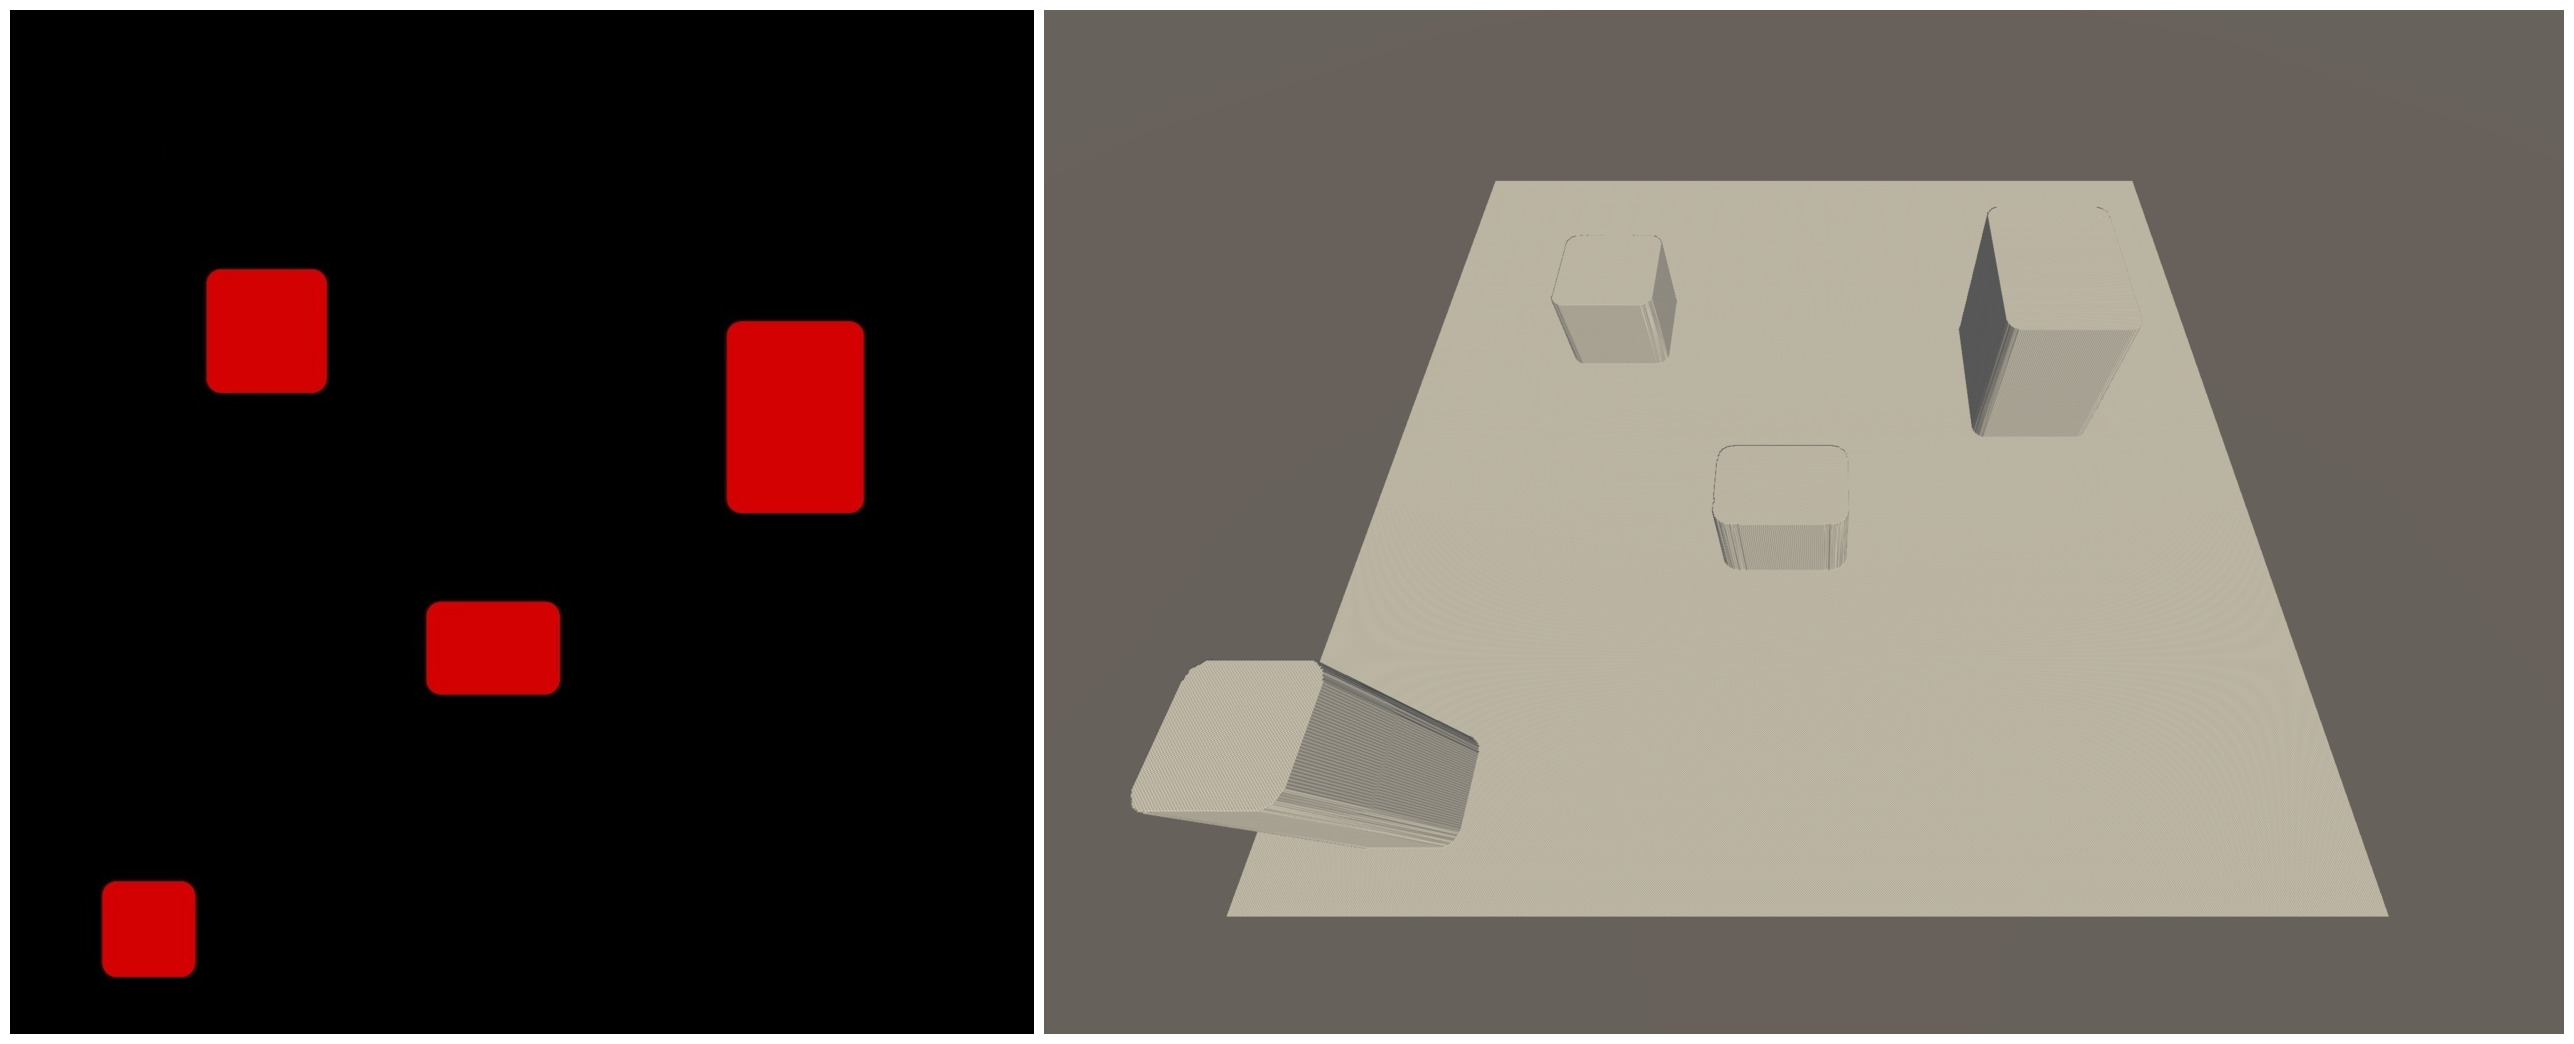
\includegraphics[width=0.7\linewidth]{img/evaluation/2/constraint_2.jpg}
    \caption{The input into our system. (Left) shows the mask texture provided. (Right) shows the set heights for the pixels mapped out by the mask texture.}
    \label{fig:constraint_2}
\end{figure}

\textbf{Manual Approach:} In Fig. \ref{fig:manual_image_2}, we can see an example of a terrain generated using the manual interaction approach.

\begin{figure}[H]
    \centering
    \includegraphics[width=0.7\linewidth]{img/evaluation/2/manual_image_2.png}
    \caption{Resulting terrain for \ref{fig:constraint_2} generated using manually set terrain operation.}
    \label{fig:manual_image_2}
\end{figure}

\textbf{IGA Approach:} In Fig. \ref{fig:iga_image_2}, we can see an example of a terrain generated using the IGA approach.

\begin{figure}[H]
    \centering
    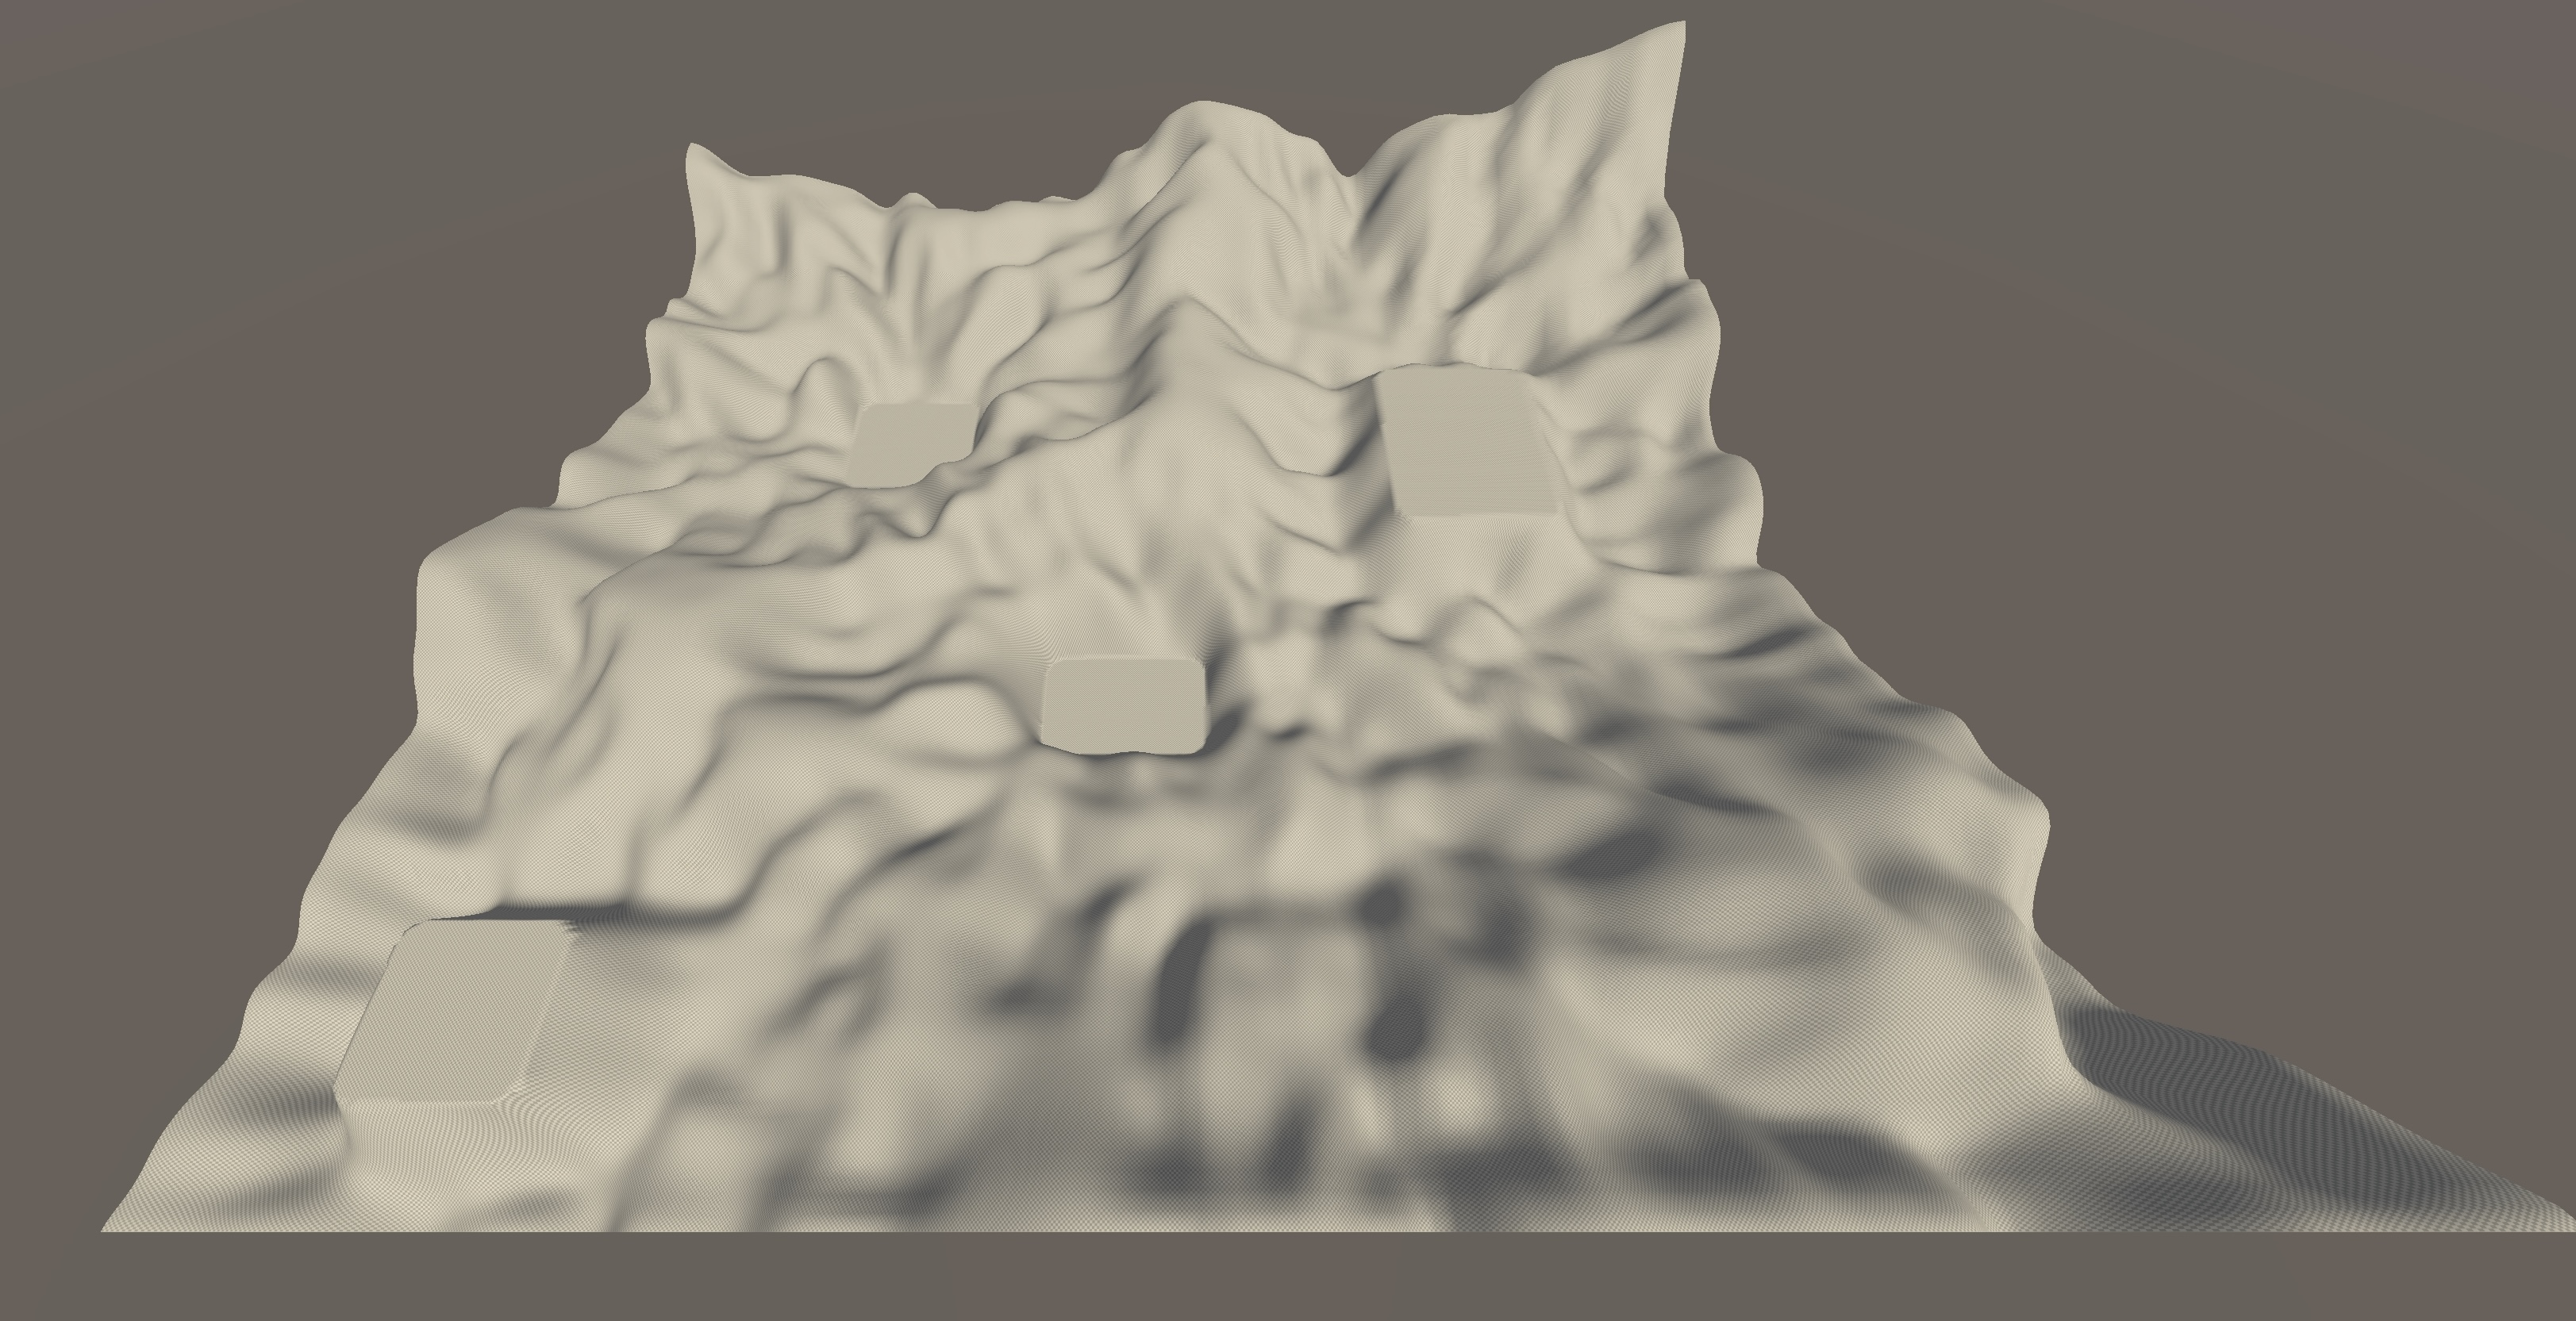
\includegraphics[width=0.6\linewidth]{img/evaluation/2/iga_image_2.jpg}
    \caption{Resulting terrain for \ref{fig:constraint_2} generated using the IGA evolution window.}
    \label{fig:iga_image_2}
\end{figure}

% Case Study 3
\subsection{River Network constraint}

This case study aims to show our system's ability to deal with constraints that could resemble a river network. A similar mask could also represent the ridge lines of a mountain range. The heights start high at the source of the river, and decrease as the river flows downhill.
In our example, we will use the constraint combination as seen in Fig. \ref{fig:constraint_3}, with the mask texture seen on the left, and the respective predefined heights seen on the right.

\begin{figure}[H]
    \centering
    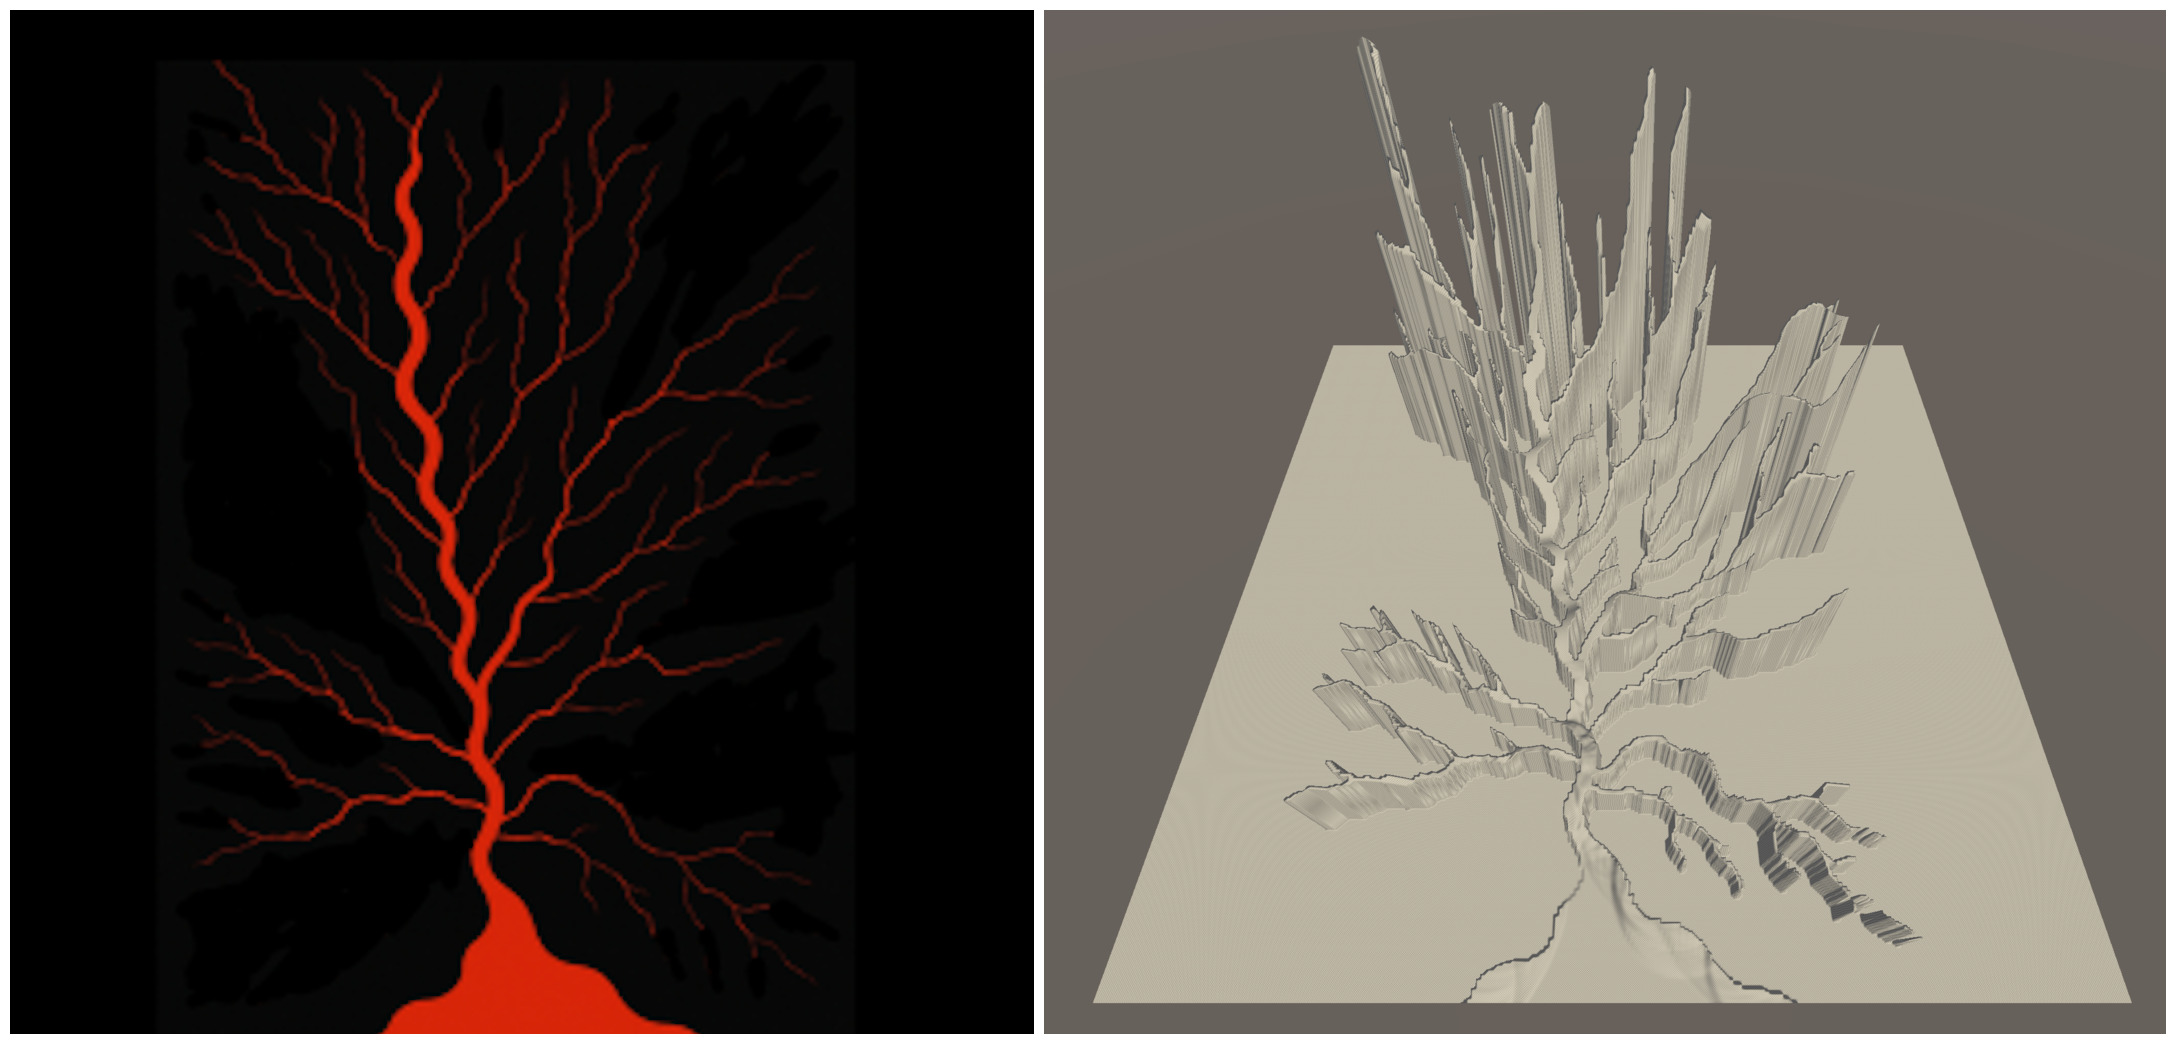
\includegraphics[width=0.6\linewidth]{img/evaluation/3/constraint_3.jpg}
    \caption{The input into our system. (Left) shows the mask texture provided. (Right) shows the set heights for the pixels mapped out by the mask texture.}
    \label{fig:constraint_3}
\end{figure}

\textbf{Manual Approach:} In Fig \ref{fig:manual_image_3}, we can see an example of a terrain generated using the manual interaction approach.

\begin{figure}[H]
    \centering
    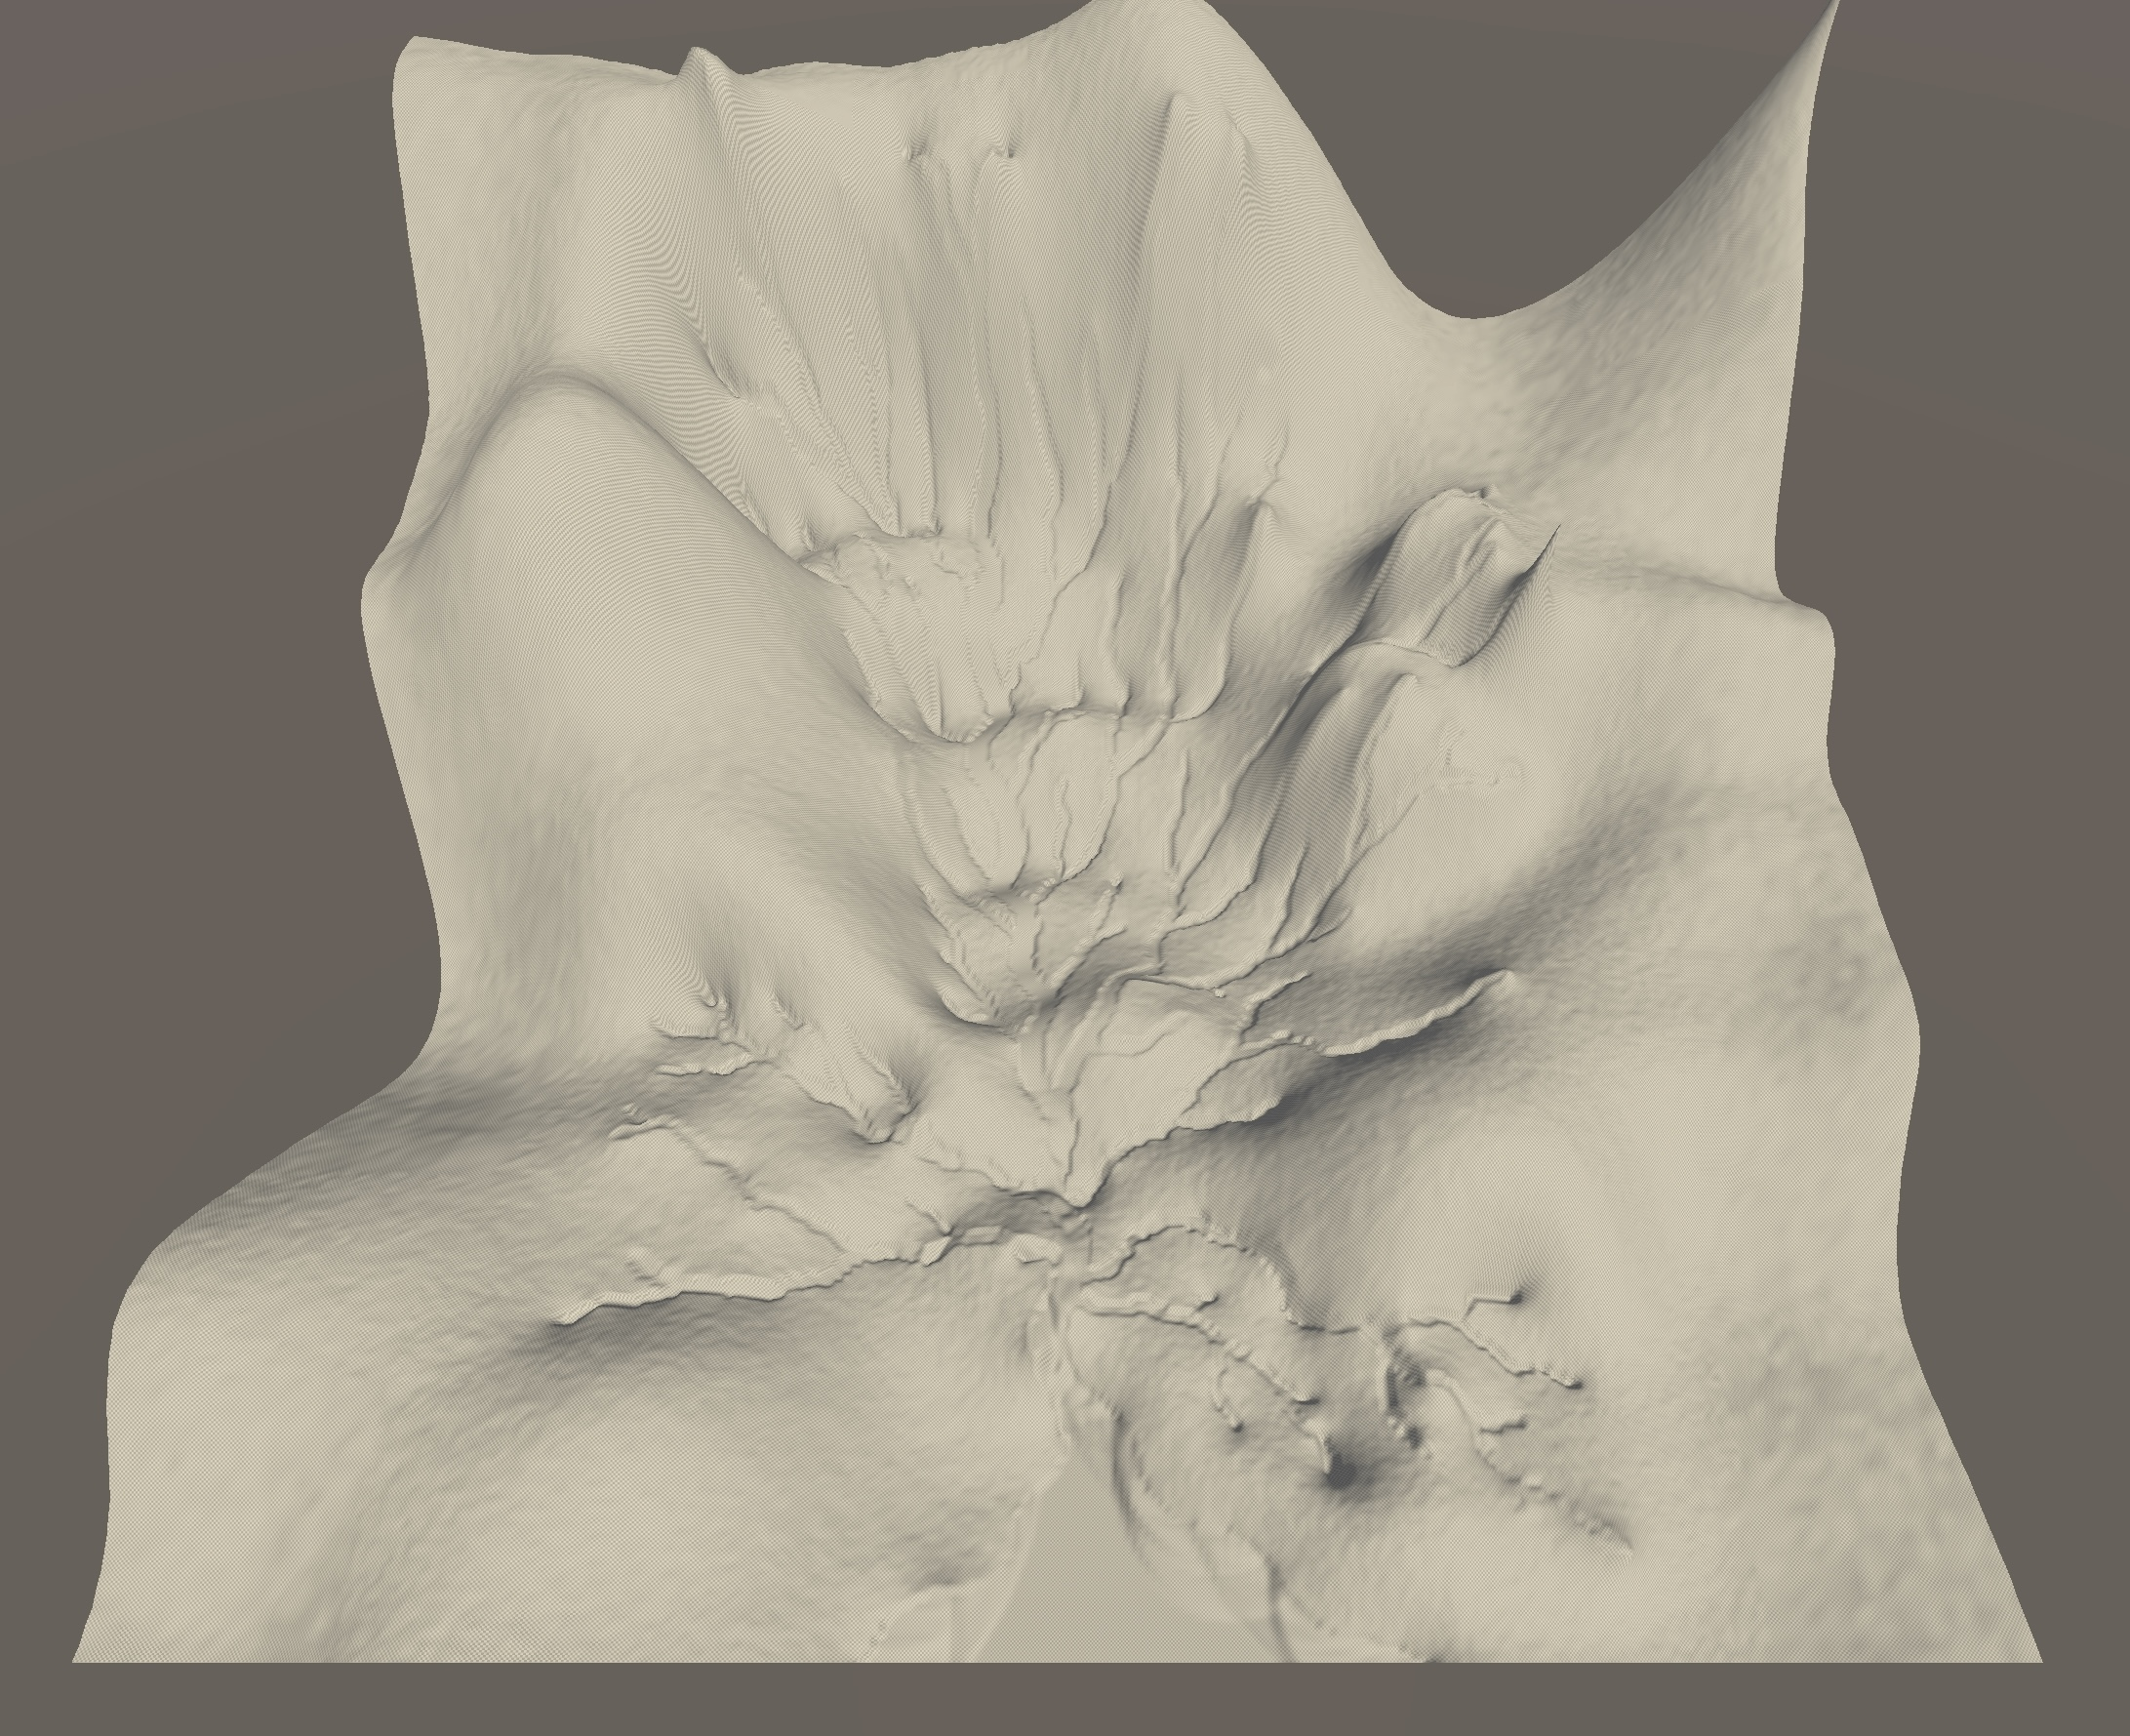
\includegraphics[width=0.5\linewidth]{img/evaluation/3/manual_image_3.jpg}
    \caption{Resulting terrain for \ref{fig:constraint_3} generated using manually set terrain operation.}
    \label{fig:manual_image_3}
\end{figure}

\textbf{IGA Approach:} In Fig. \ref{fig:iga_image_3}, we can see an example of a terrain generated using the IGA approach.

\begin{figure}[h!]
    \centering
    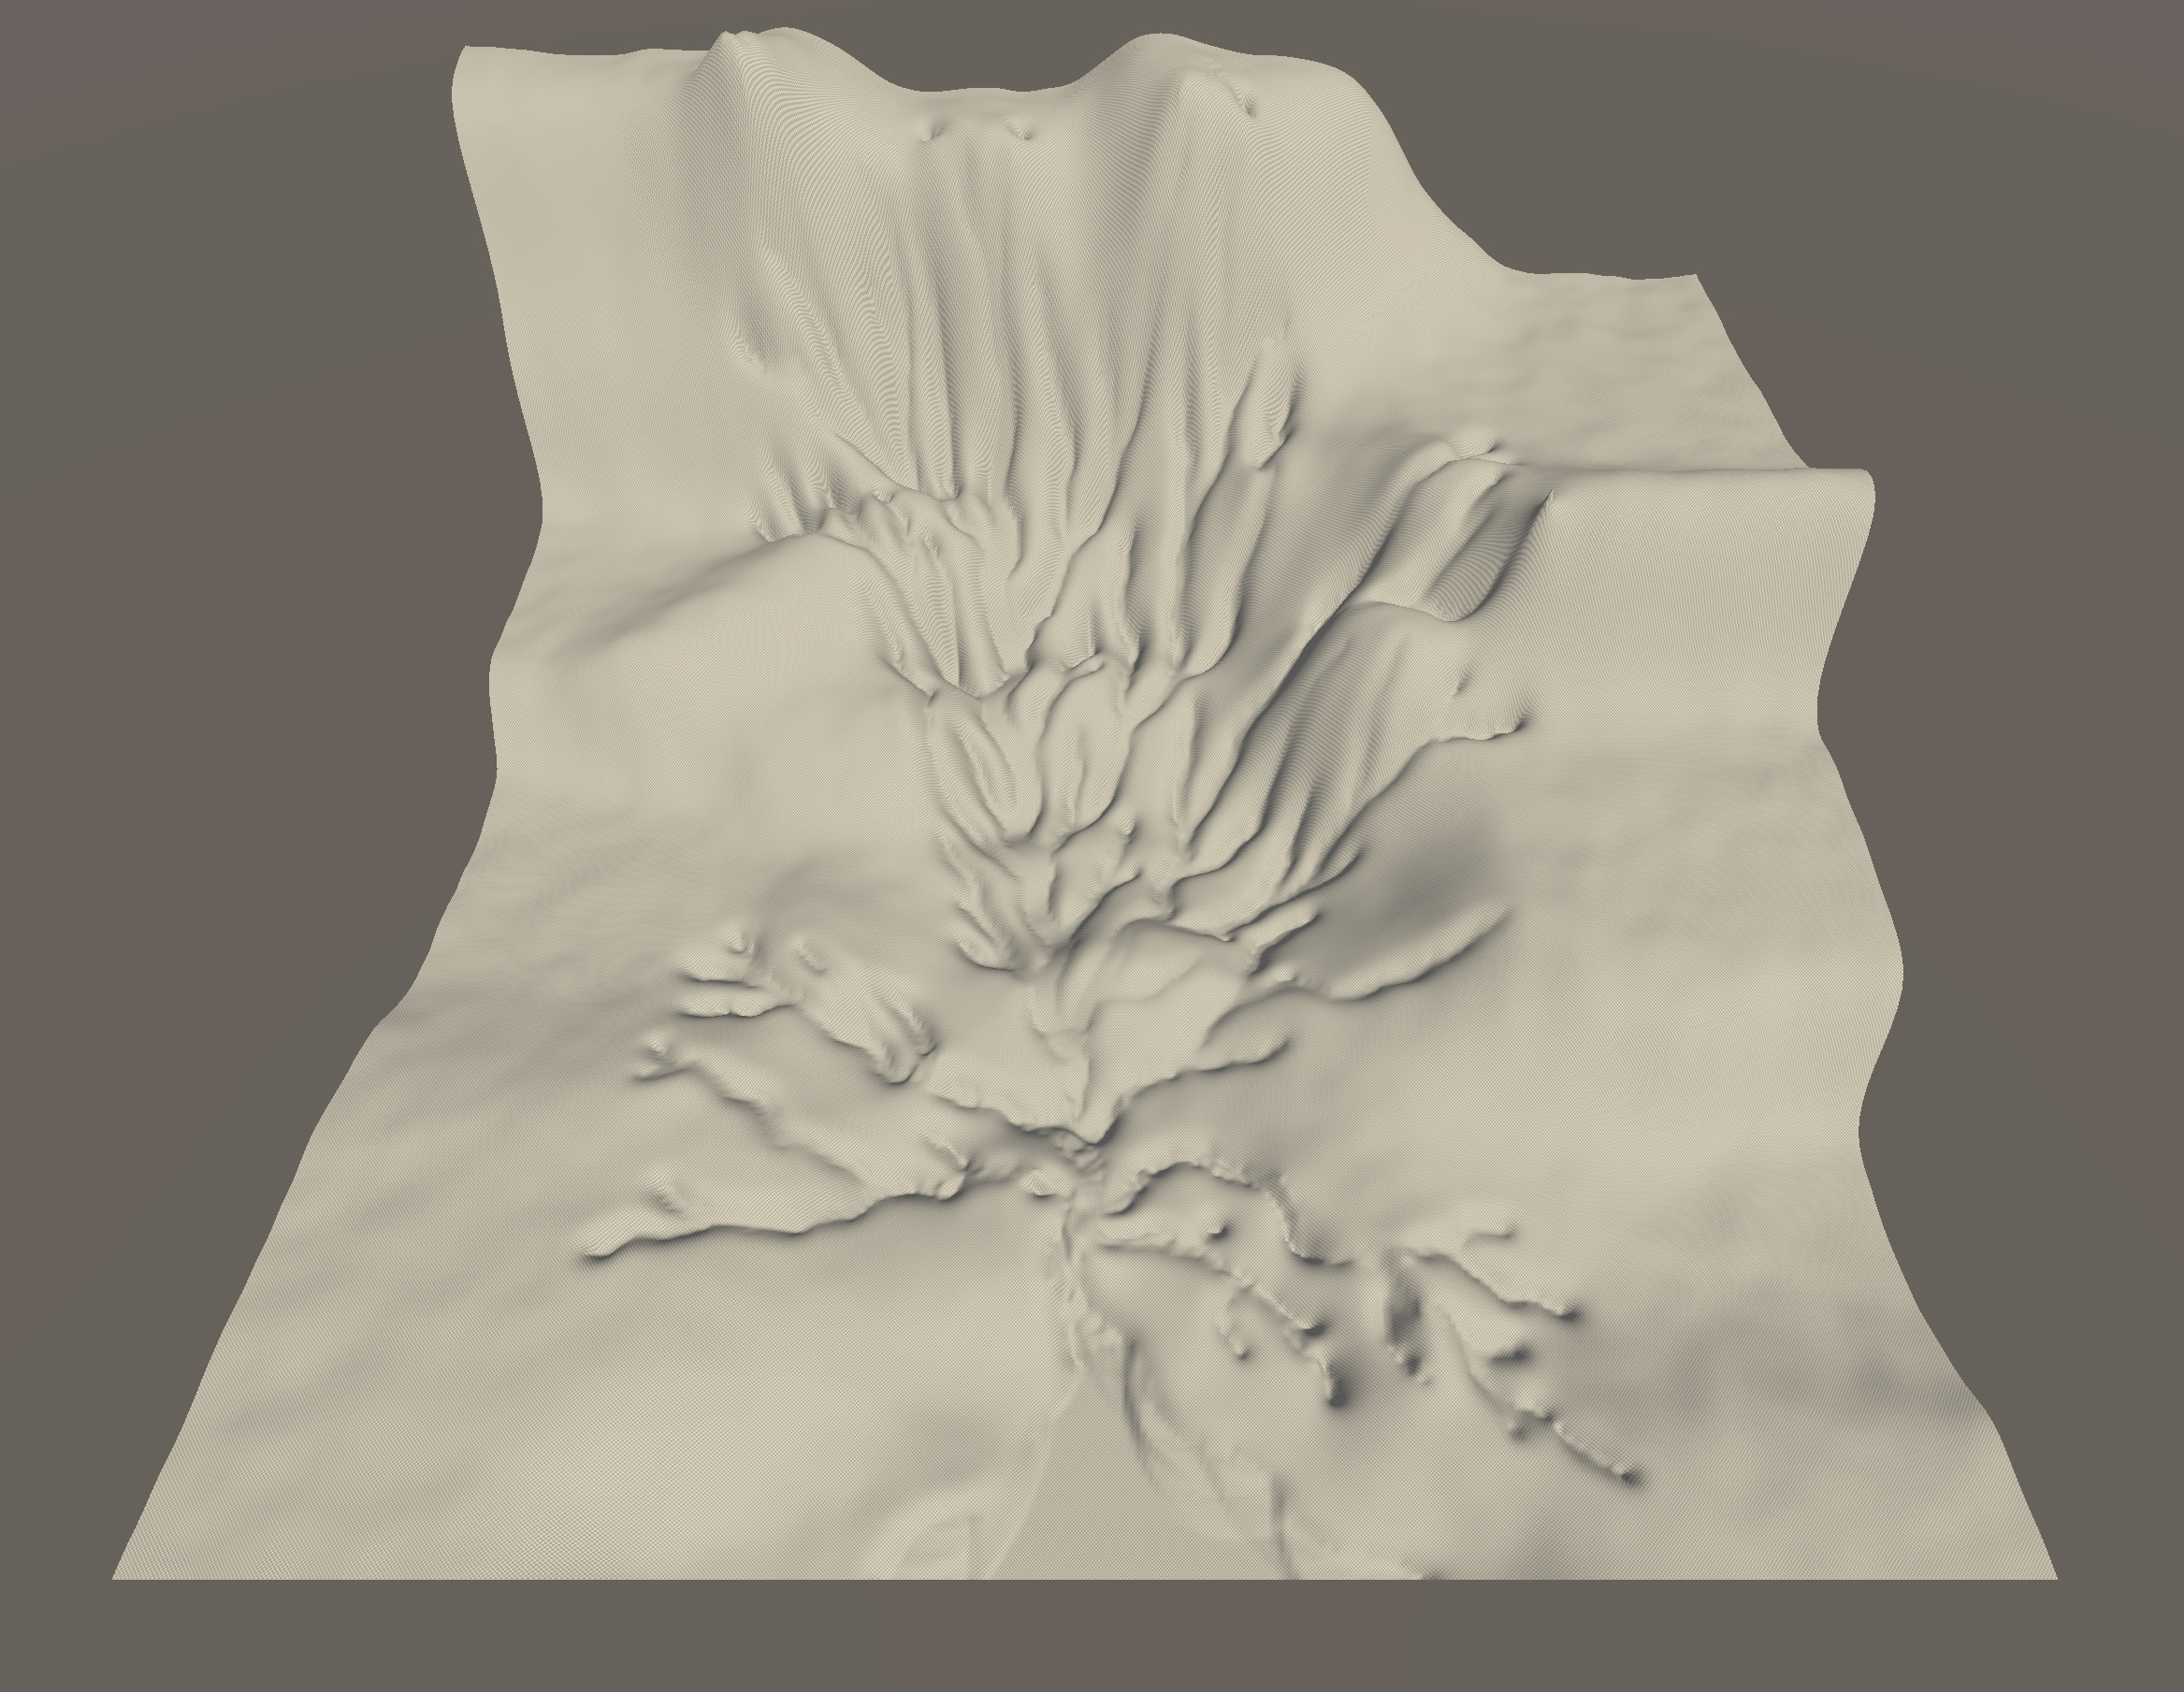
\includegraphics[width=0.5\linewidth]{img/evaluation/3/iga_image_3.jpg}
    \caption{Resulting terrain for \ref{fig:constraint_3} generated using the IGA evolution window.}
    \label{fig:iga_image_3}
\end{figure}


% Case Study 4
\subsection{Island/Coastline network constraint}

This case study aims to show our system's ability to deal with generating the land bordering bodies of water. The constrained area represents flat water, and then we aim to modify the island/land to have natural coastlines, which tend to have smooth transitions into the water.
In our example, we will use the constraint combination as seen in Fig. \ref{fig:constraint_4}:

\begin{figure}[H]
    \centering
    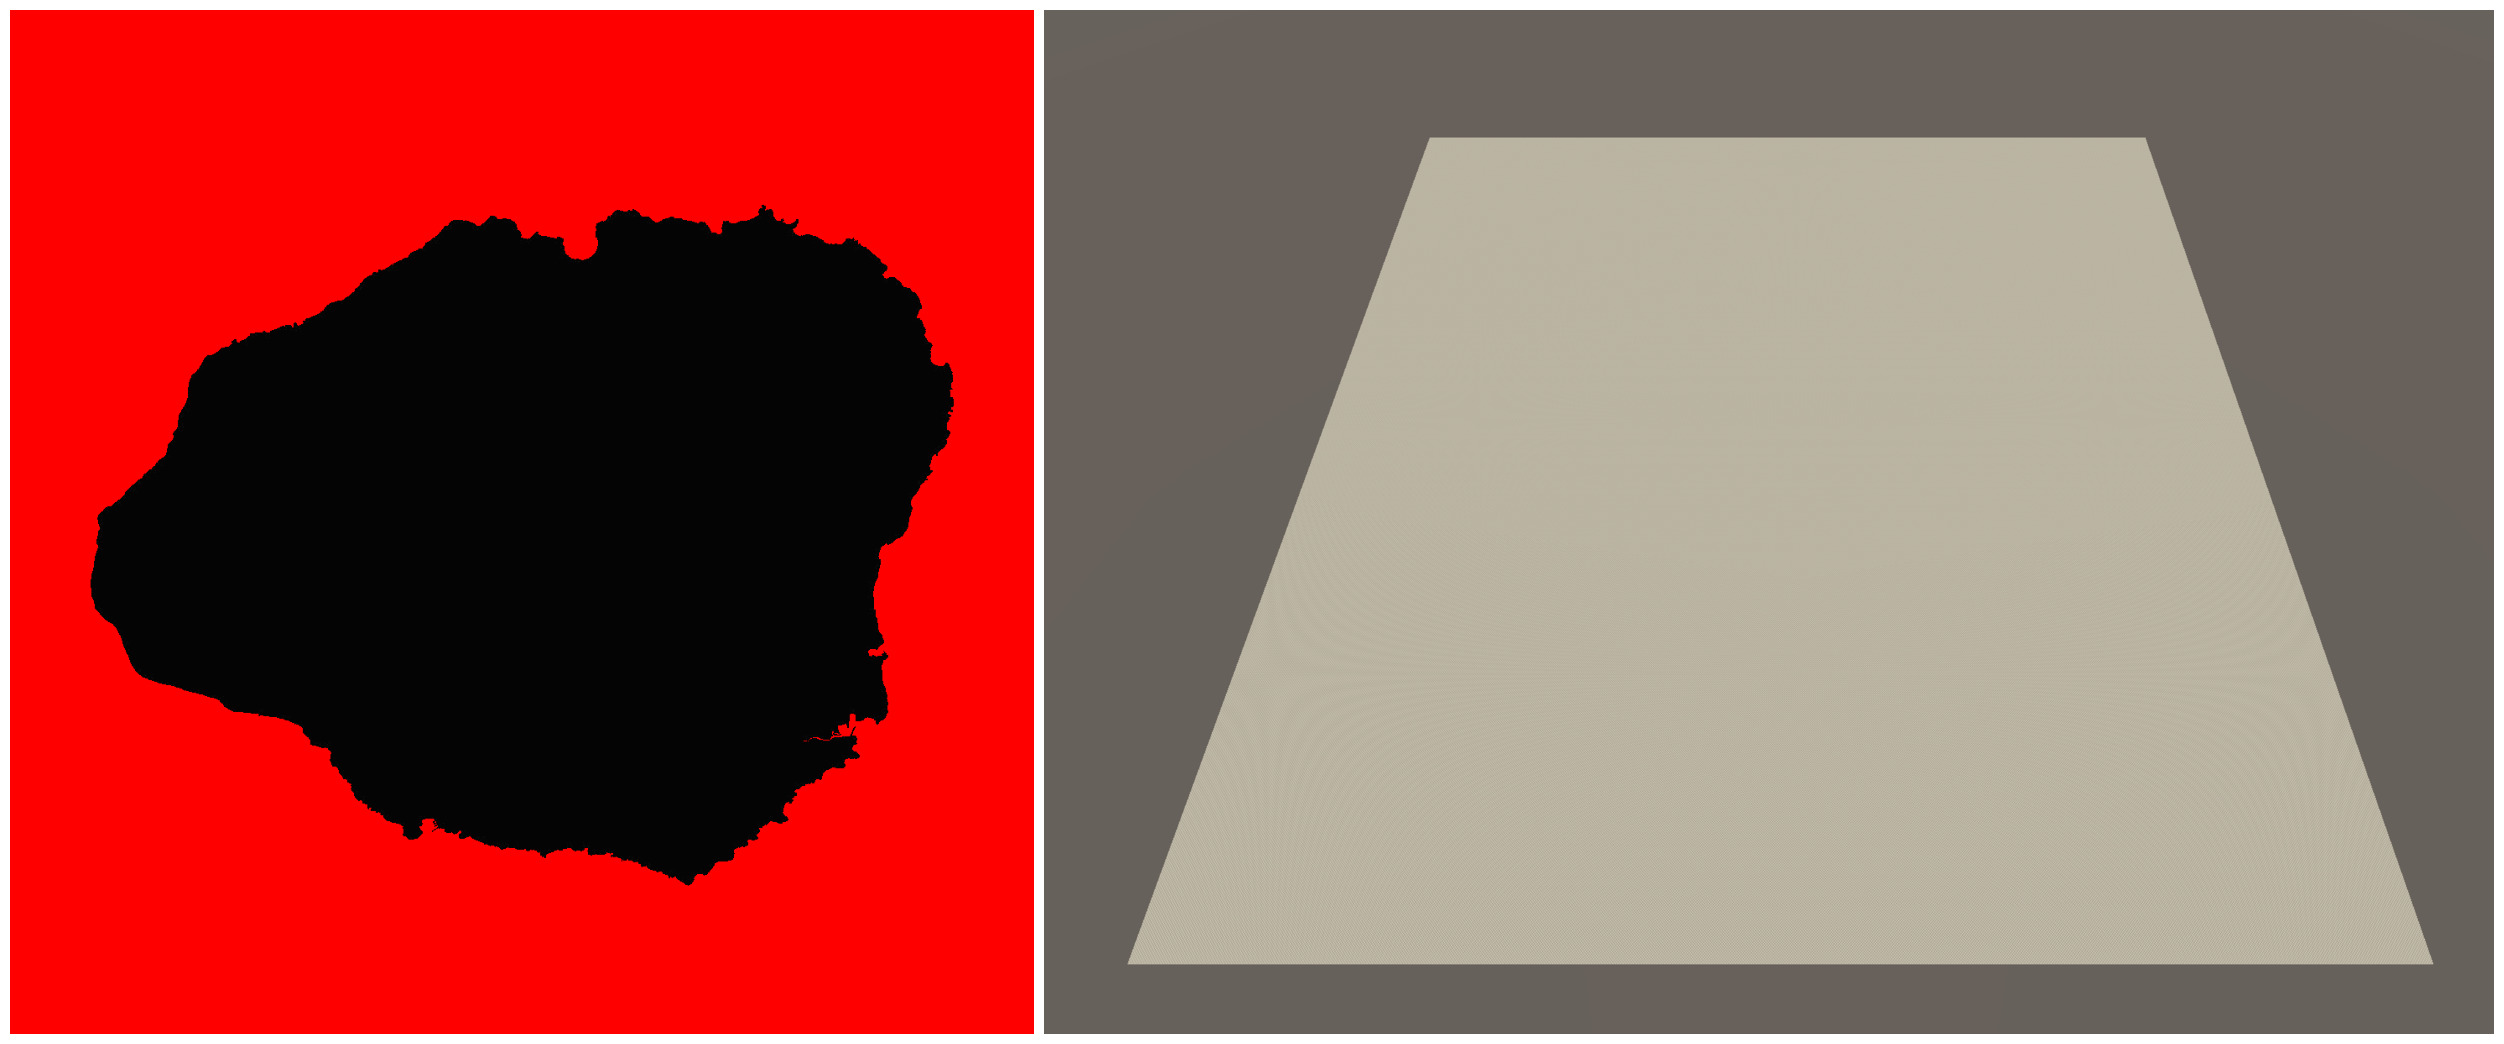
\includegraphics[width=0.5\linewidth]{img/evaluation/4/constraint_4.jpg}
    \caption{The input into our system. (Left) shows the mask texture provided. (Right) shows the set heights for the pixels mapped out by the mask texture. }
    \label{fig:constraint_4}
\end{figure}

\textbf{Manual Approach:} In Fig \ref{fig:manual_image_4}, we can see an example of a terrain generated using the manual interaction approach.

\begin{figure}[H]
    \centering
    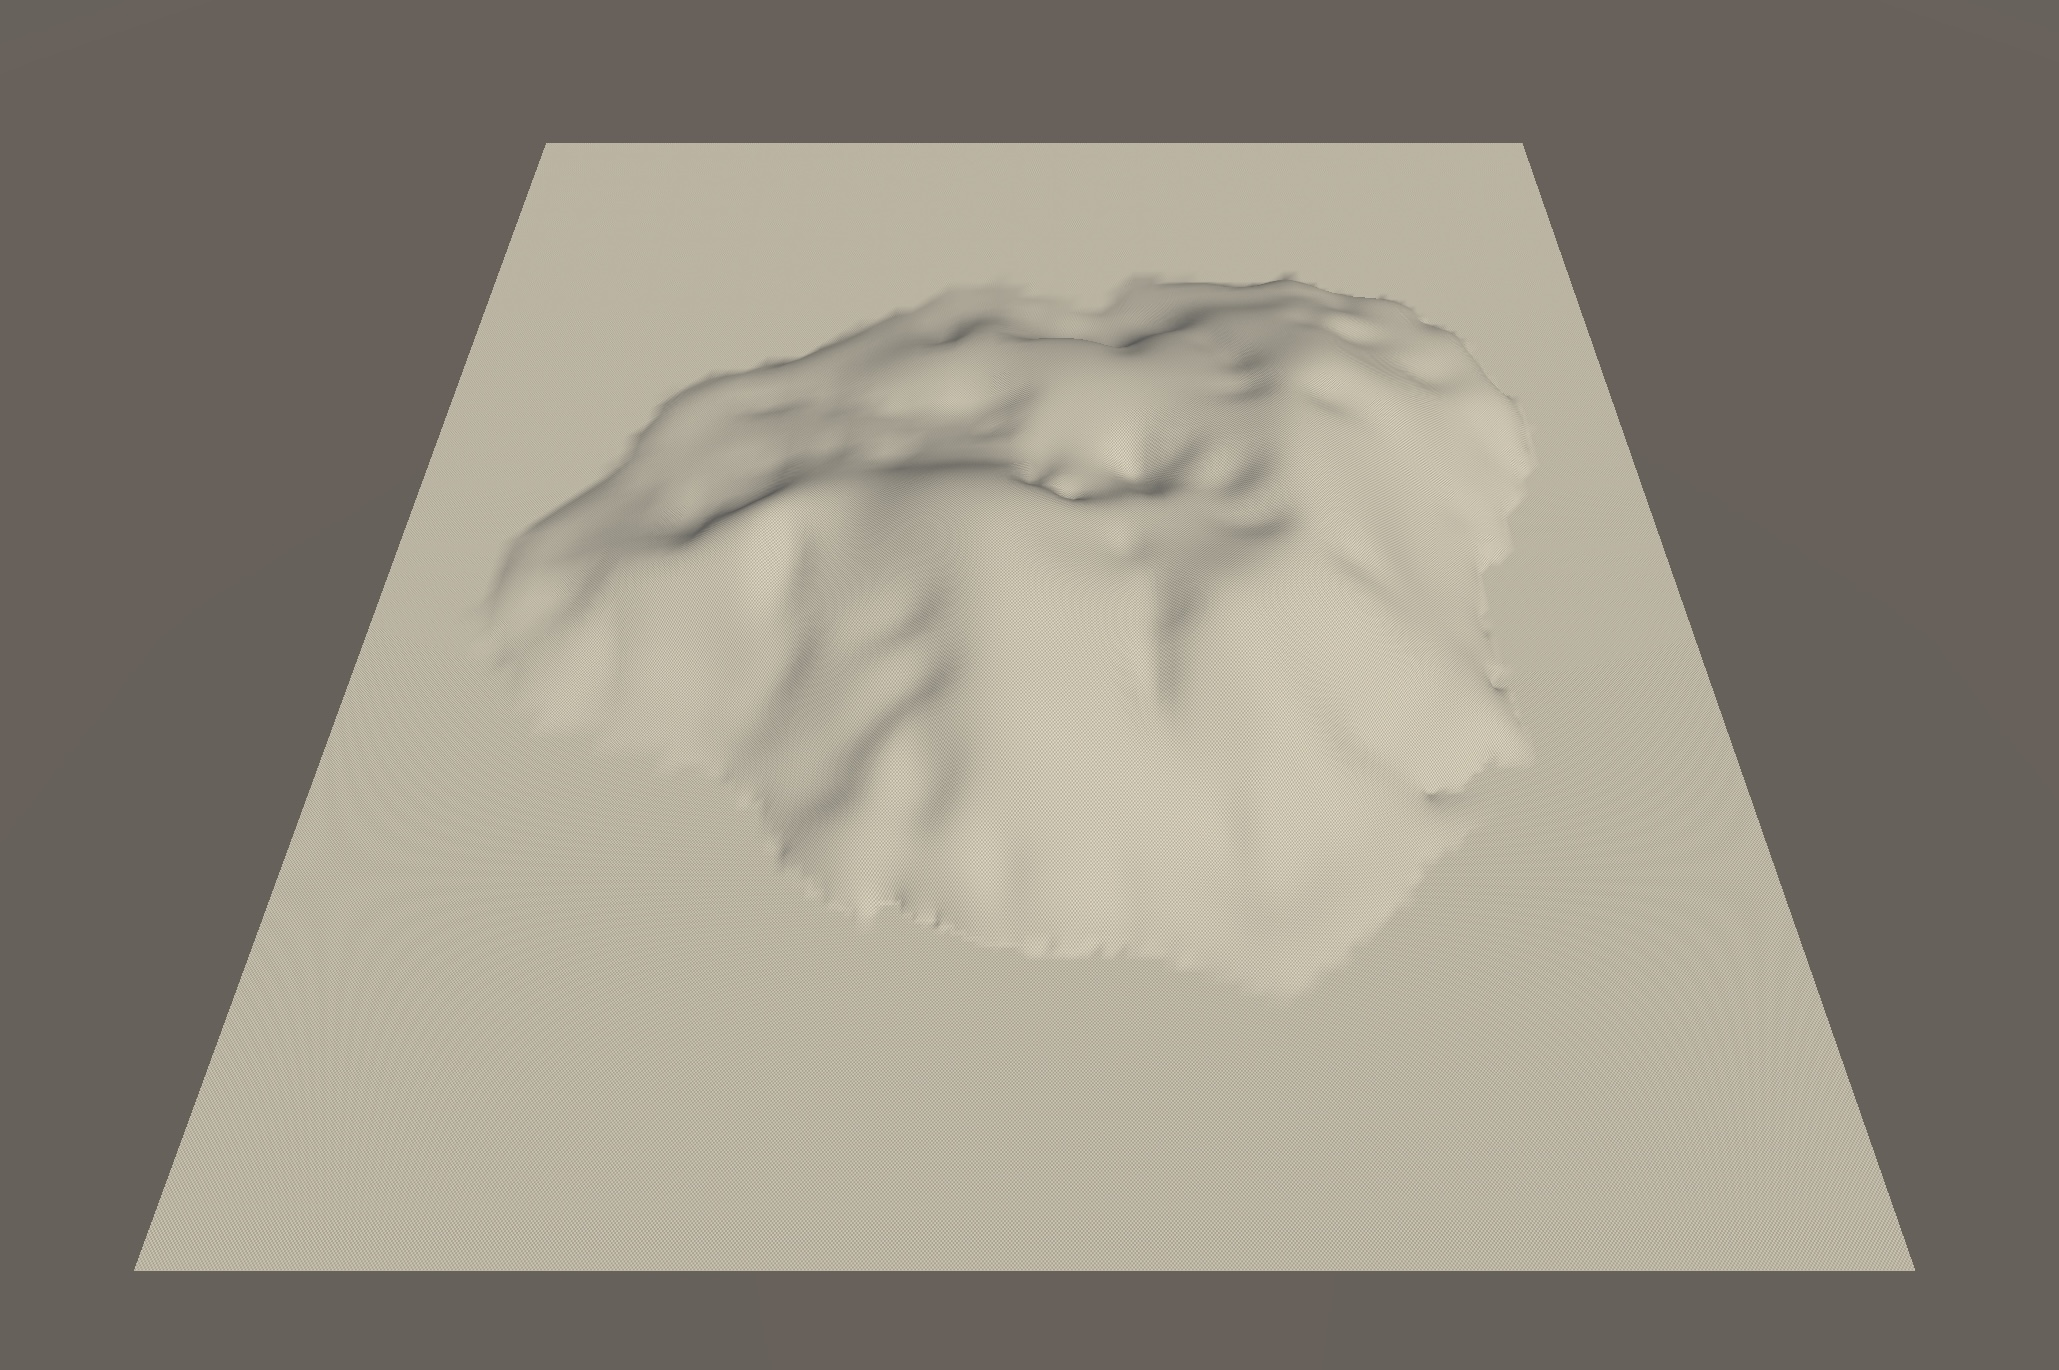
\includegraphics[width=0.5\linewidth]{img/evaluation/4/manual_image_4.jpg}
    \caption{Resulting terrain for \ref{fig:constraint_4} generated using manually set terrain operations.}
    \label{fig:manual_image_4}
\end{figure}

\textbf{IGA Approach:} In Fig. \ref{fig:iga_image_4}, we can see an example of a terrain generated using the IGA approach.

\begin{figure}[H]
    \centering
    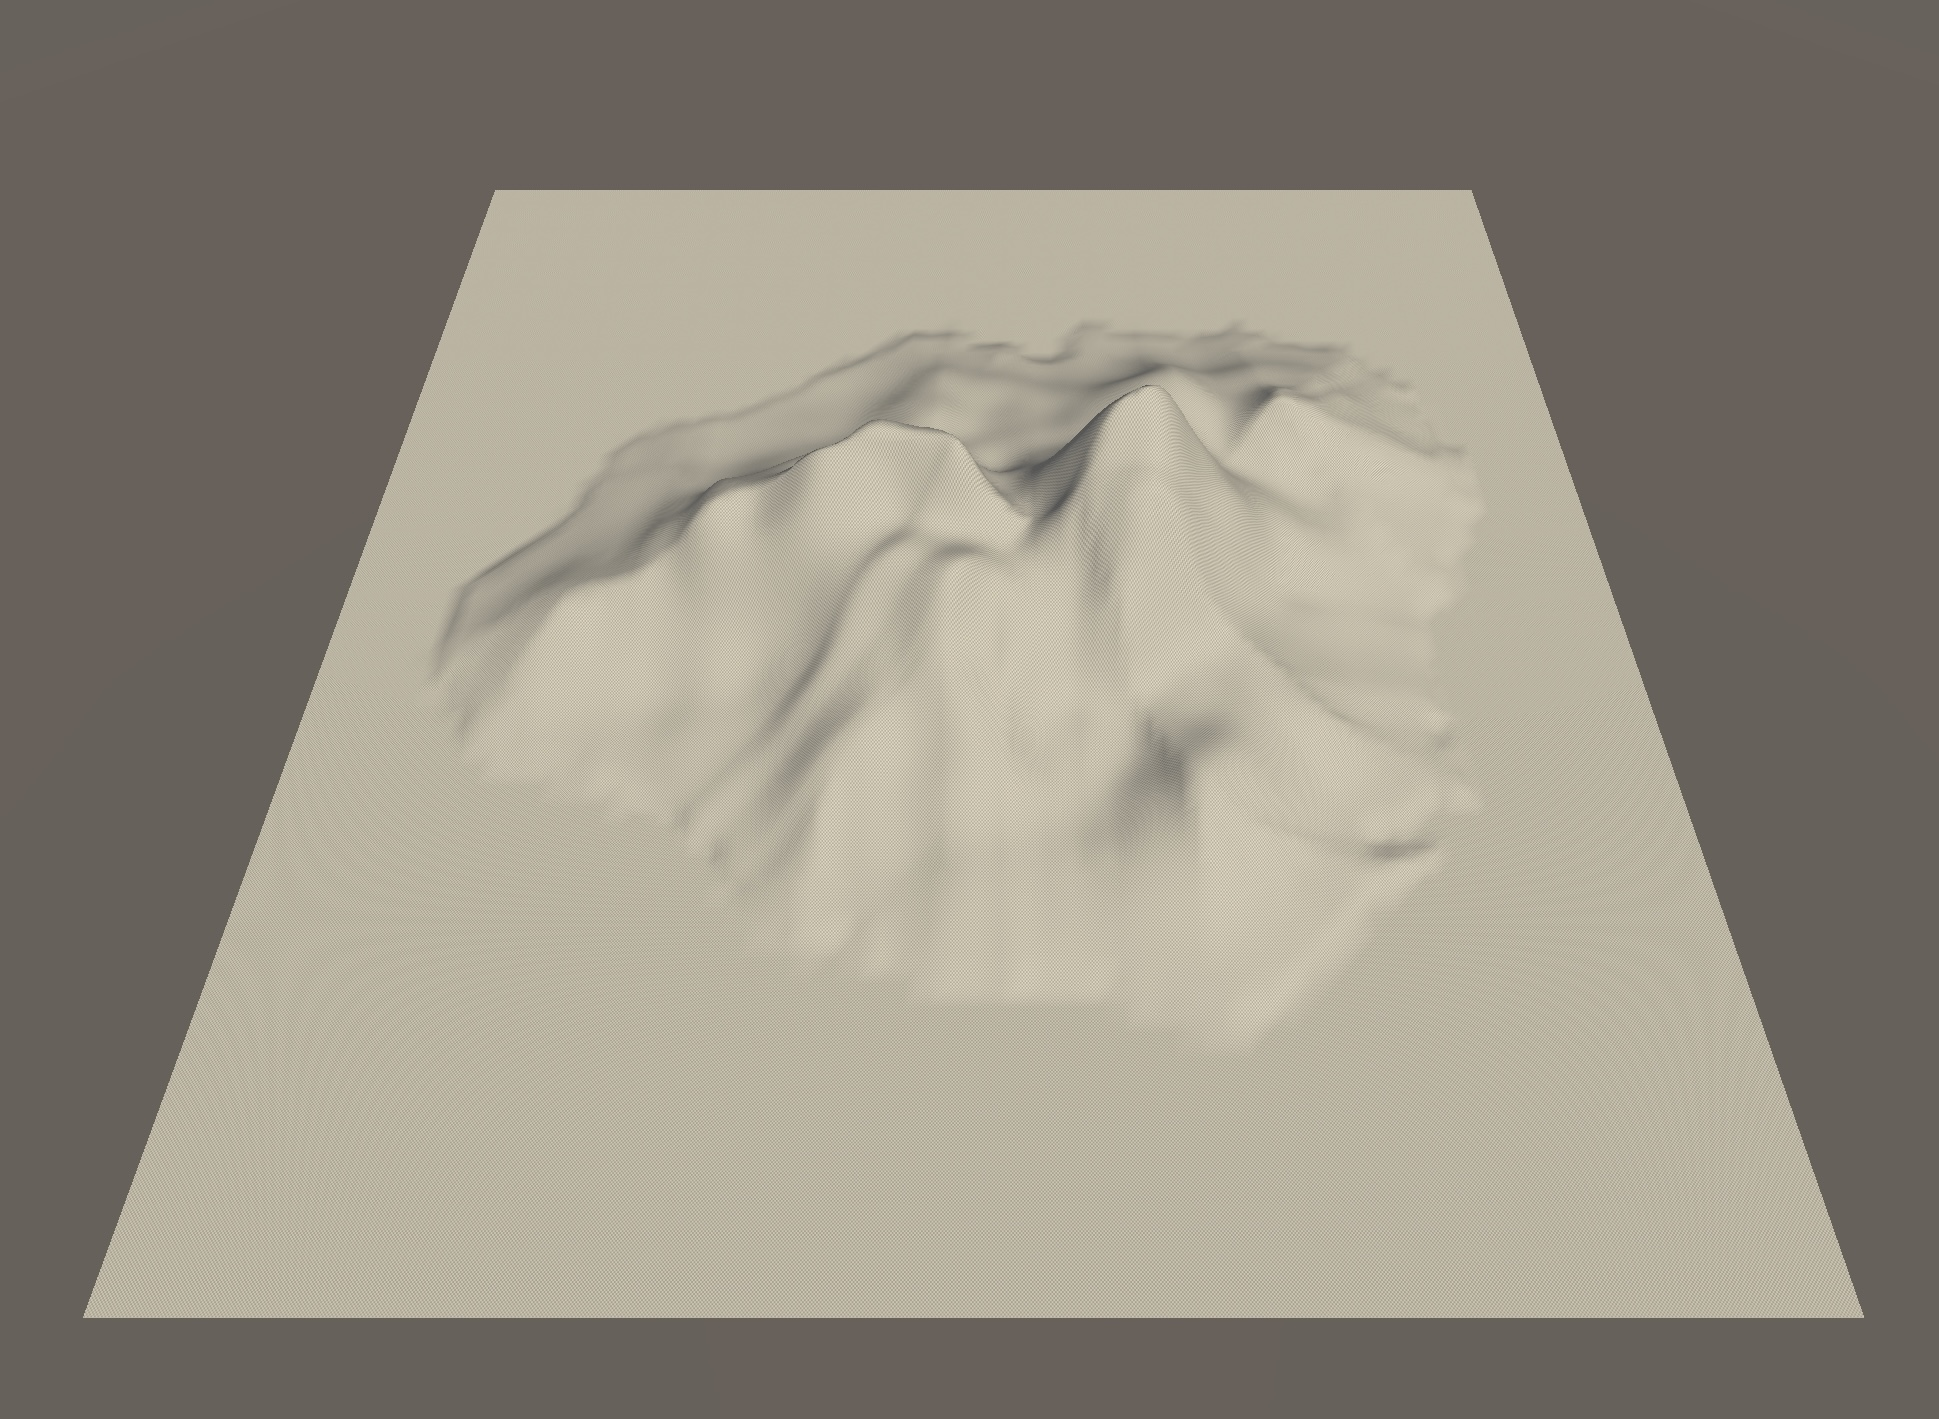
\includegraphics[width=0.55\linewidth]{img/evaluation/4/iga_image_4.jpg}
    \caption{Resulting terrain for \ref{fig:constraint_4} generated using the IGA evolution window.}
    \label{fig:iga_image_4}
\end{figure}

% Case Study 5
\subsection{Combination of man-made and natural features constraint}

This case study aims to show our systems ability to deal with a combination of different use cases in one terrain. Here, we interpret part of the constraint to represent a building foundation, which has connecting roads (both man-made) as well as the other parts to represent a dam and a mountain (natural features). We aim for our system to fill in the heights of the modifiable areas to connect all these constrained areas in a coherent and natural way.

In our example, we will use the constraint combination as seen in Fig. \ref{fig:constraint_5}, with the mask texture seen on the left, and the respective predefined heights seen on the right.

\begin{figure}[H]
    \centering
    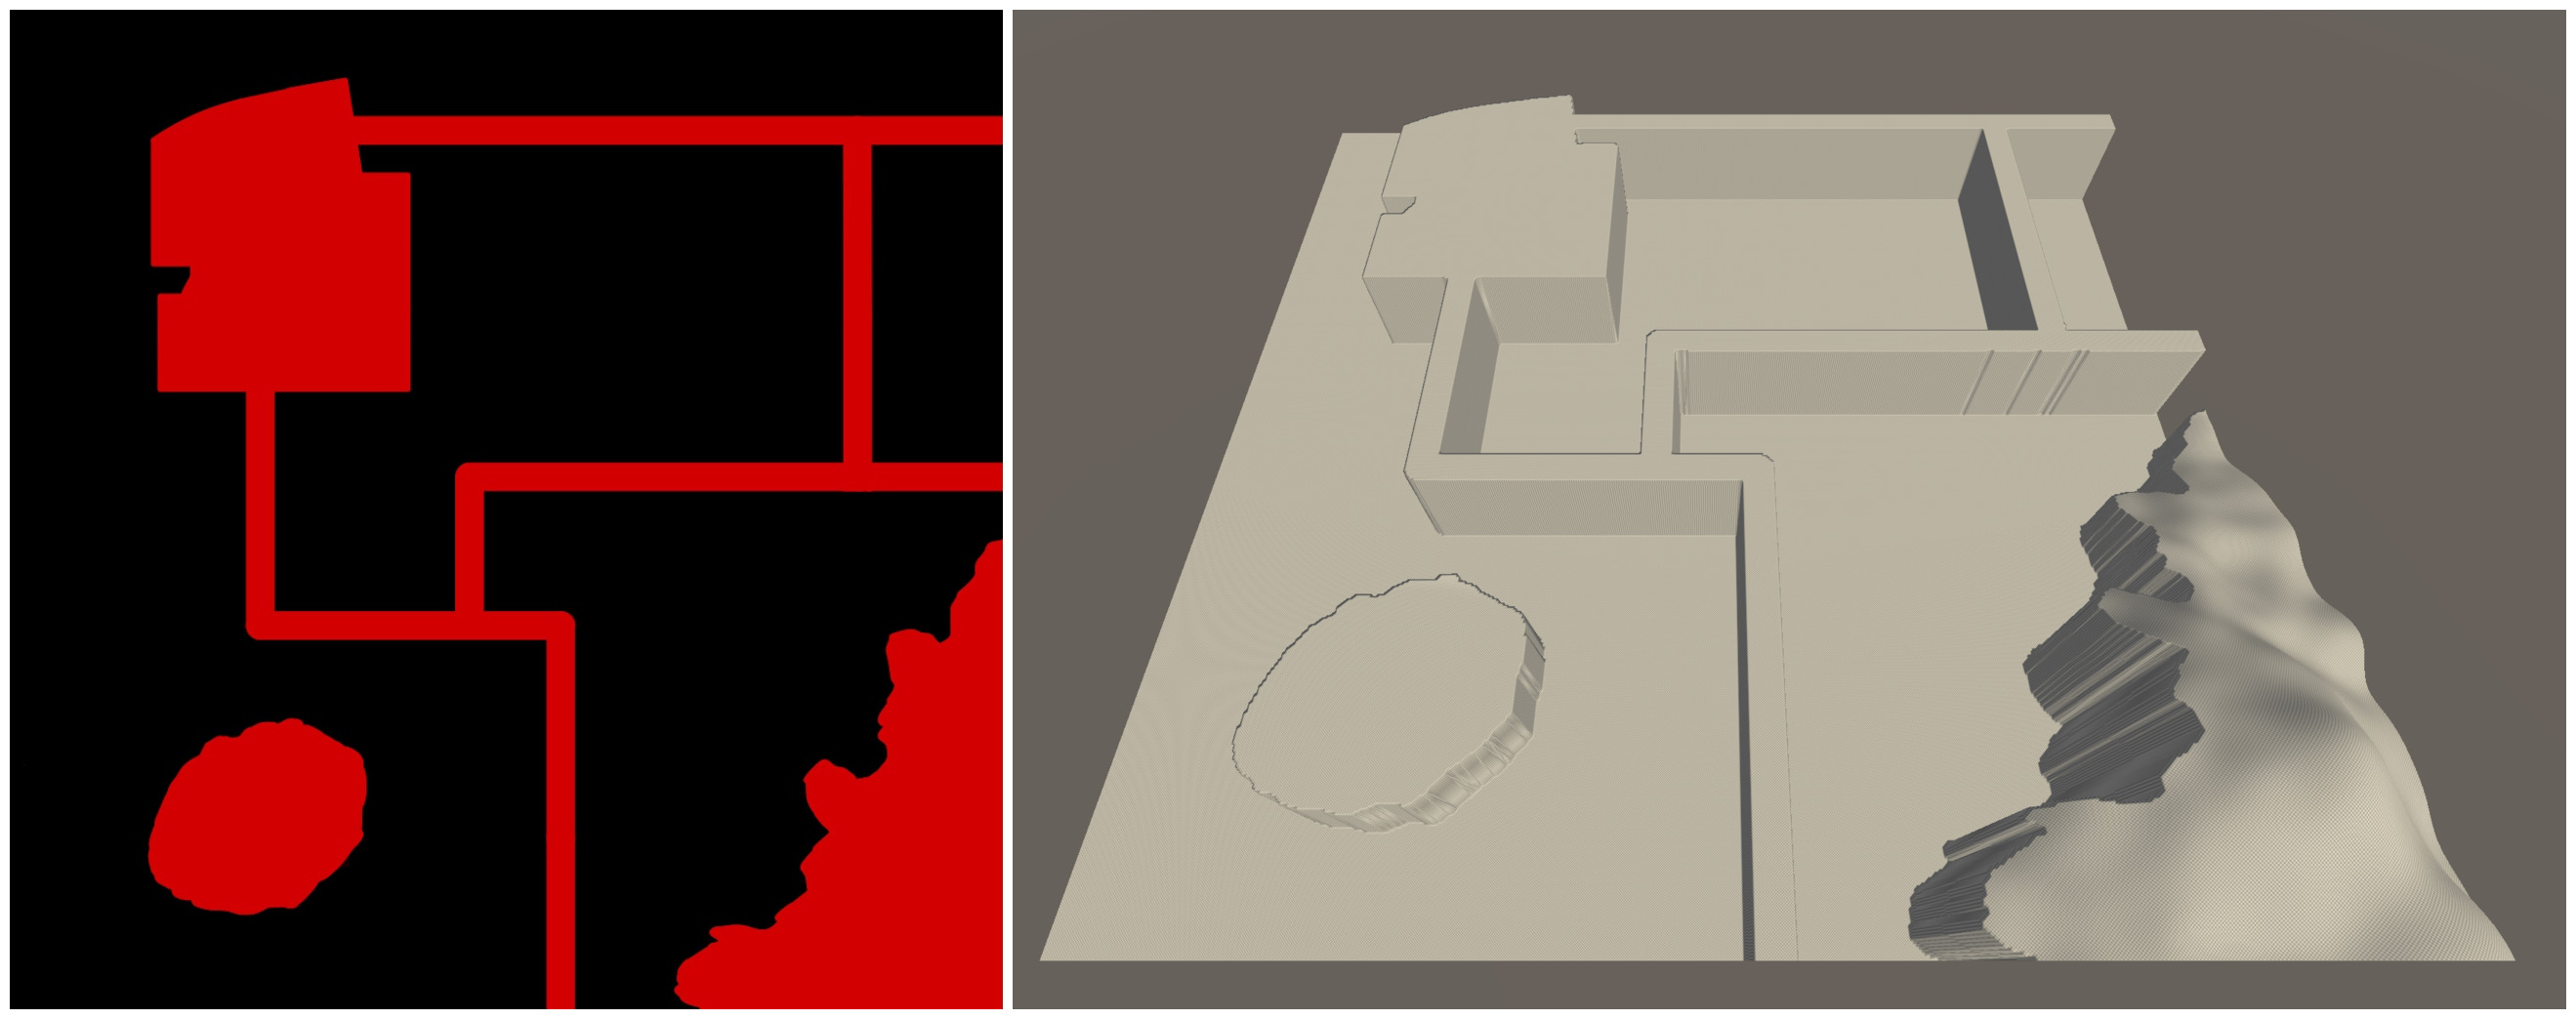
\includegraphics[width=0.75\linewidth]{img/evaluation/5/constraint_5.jpg}
    \caption{The input into our system. (Left) shows the mask texture provided. (Right) shows the set heights for the pixels mapped out by the mask texture.}
    \label{fig:constraint_5}
\end{figure}

\textbf{Manual Approach:} In Fig. \ref{fig:manual_image_5}, we can see an example of a terrain generated using the manual interaction approach.

\begin{figure}[H]
    \centering
    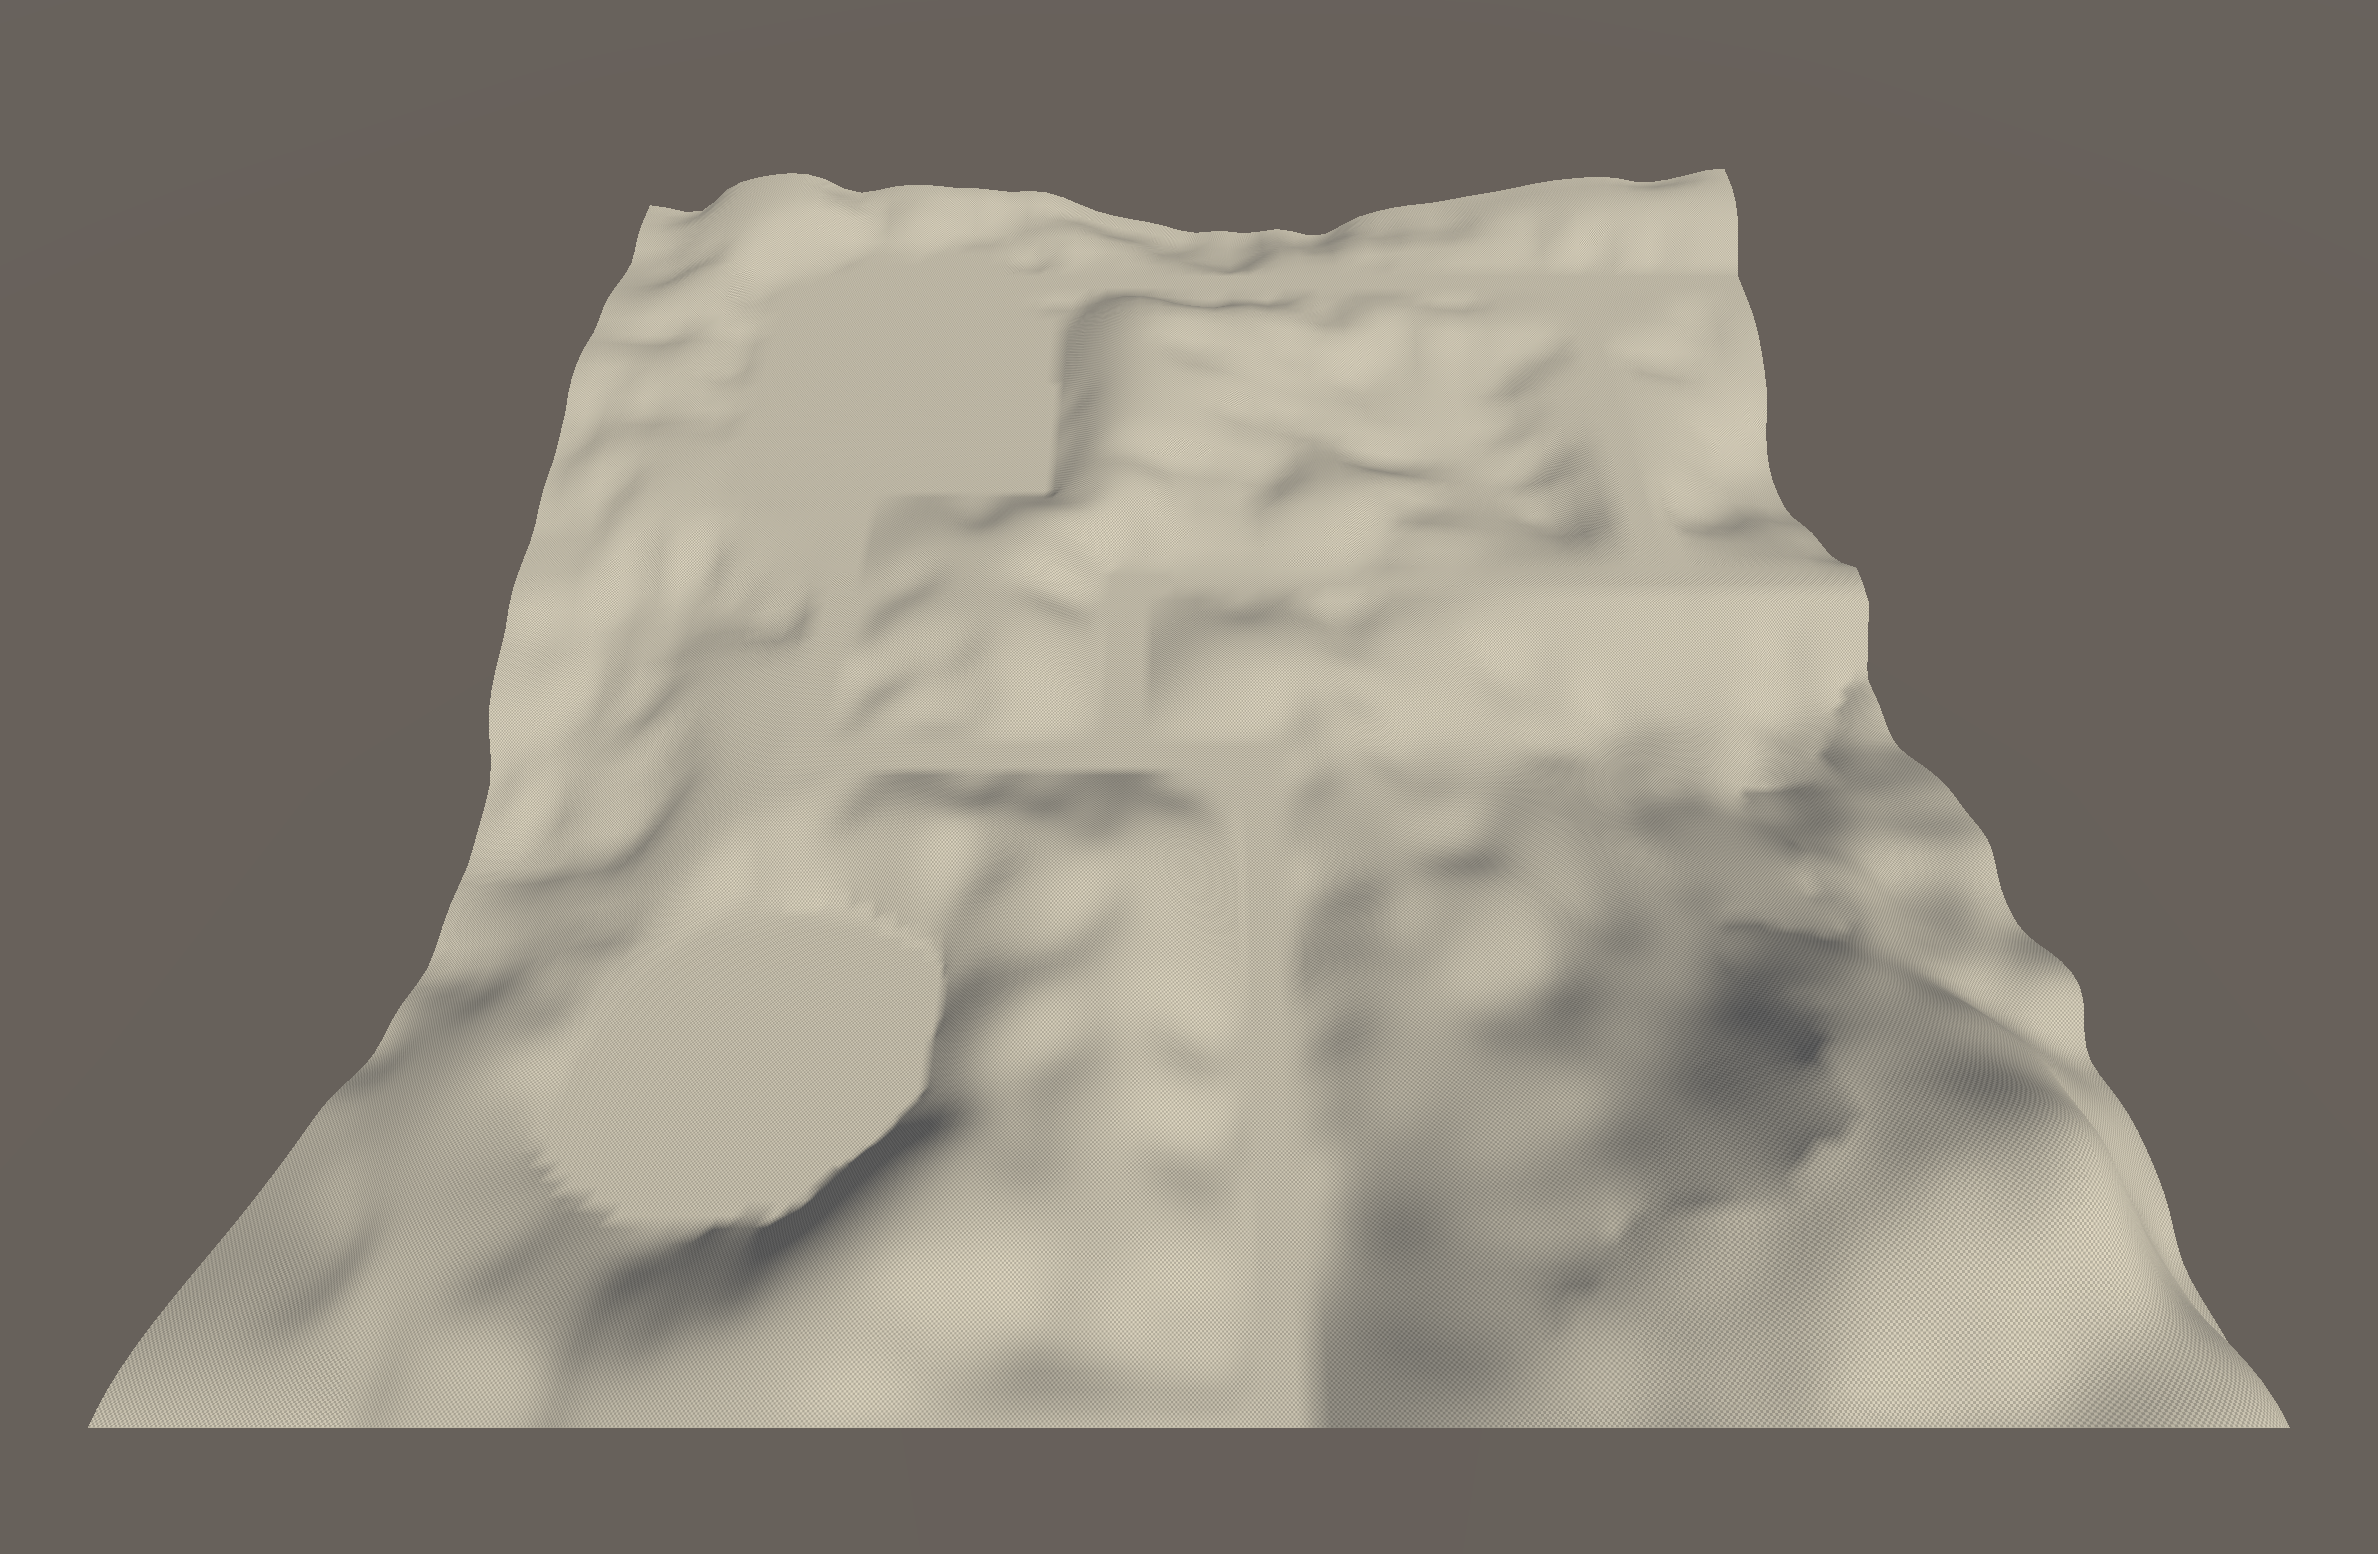
\includegraphics[width=0.55\linewidth]{img/evaluation/5/manual_image_5.png}
    \caption{Resulting terrain for \ref{fig:constraint_5} generated using manually set terrain operations.}
    \label{fig:manual_image_5}
\end{figure}

\textbf{IGA Approach:} In Fig. \ref{fig:iga_image_5}, we can see an example of a terrain generated using the IGA approach.

\begin{figure}[H]
    \centering
    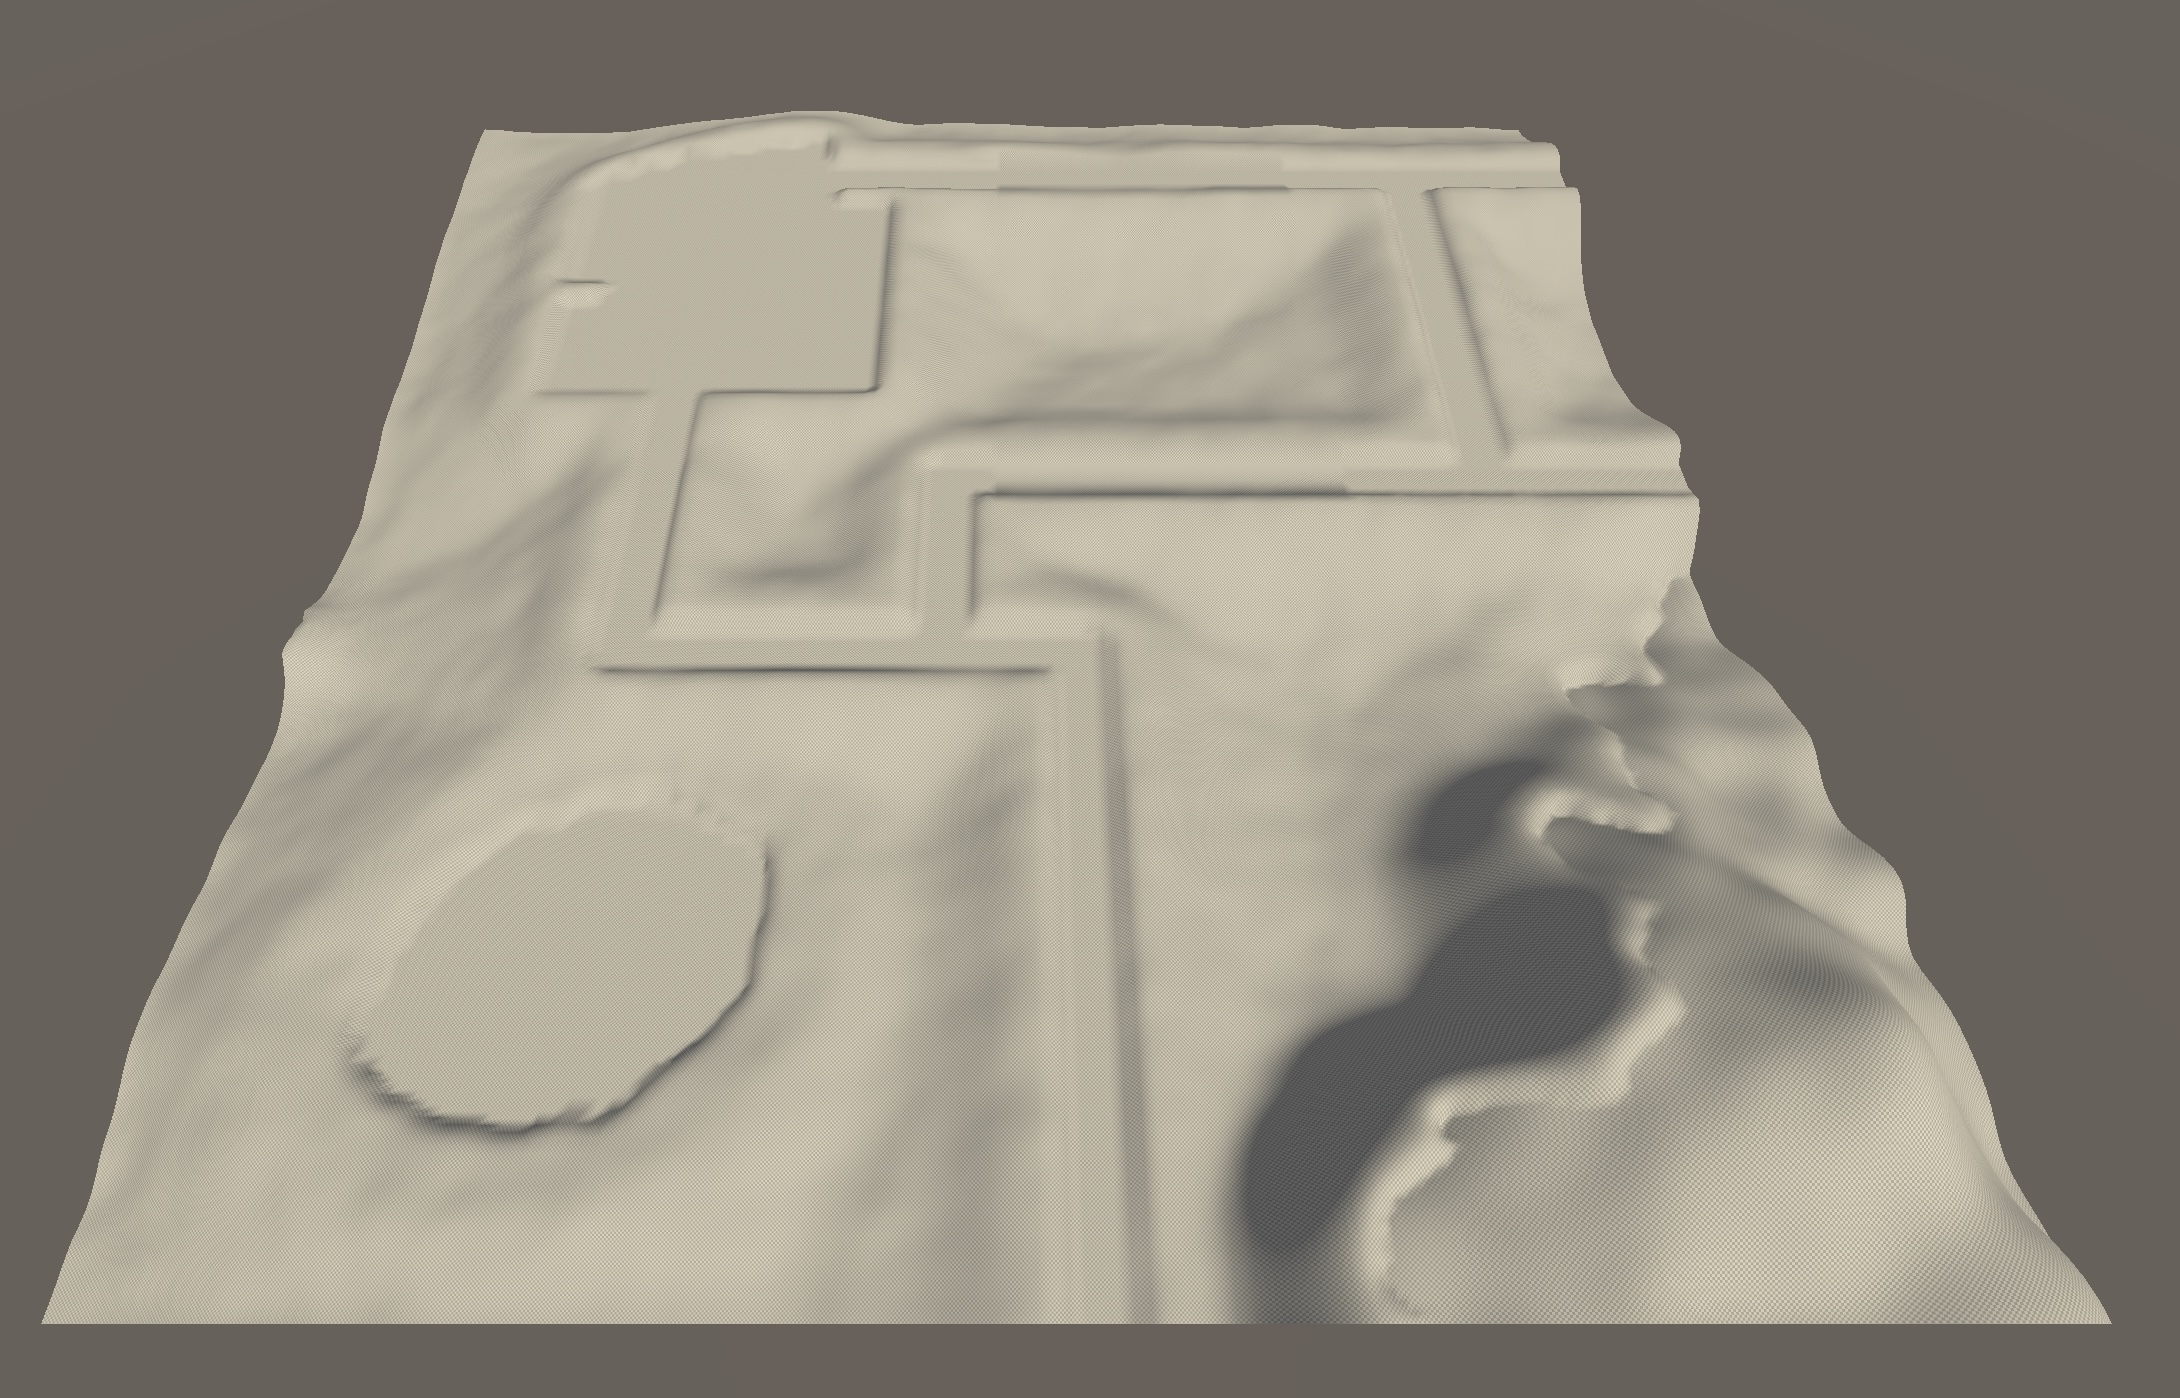
\includegraphics[width=0.55\linewidth]{img/evaluation/5/iga_image_5.jpg}
    \caption{Resulting terrain for \ref{fig:constraint_5} generated using the IGA evolution window.}
    \label{fig:iga_image_5}
\end{figure}


\section{Visual Analysis}

\subsection{Our Own Analysis of Case Studies}

Evaluating our results across the five case studies according to the visual criteria established in Section \ref{visual_crit}, we observe several noteworthy patterns and achievements in our distance-based approach.

\textbf{Smooth Transitions:} Our system demonstrates excellent performance in creating seamless blending between fixed and procedurally generated areas. This is particularly evident in the foundations constraint case study (Figure \ref{fig:manual_image_2}), where the original constraint boundaries become virtually invisible, fully integrated into the surrounding terrain. Across all case studies, we consistently avoid sharp transitions at constraint boundaries, achieving the natural flow that was our primary objective. The most challenging scenario occurred in the combination constraint case study using the IGA approach (Figure \ref{fig:iga_image_5}), where blending into the predefined mountain in the bottom-right corner proved more difficult, though still achieving acceptable integration.

\textbf{Geological Possibility:} Our generated terrains consistently exhibit formations that could feasibly exist in nature. The island/coastline constraint case study (Figures \ref{fig:manual_image_4} and \ref{fig:iga_image_4}) particularly excels in this regard, creating realistic coastal transitions that mirror natural shoreline formations. However, we observe that the river constraint generated using the IGA approach (Figure \ref{fig:iga_image_3}) occasionally exhibits patterns that appear more algorithmically generated, suggesting that our evolutionary approach may require further refinement for certain constraint types.

\textbf{Contextual Coherence:} The road/path network constraint case study (Figures \ref{fig:manual_image_1} and \ref{fig:iga_image_1}) demonstrates exceptional contextual integration, where the road infrastructure appears naturally embedded within the landscape rather than artificially imposed. This success extends to our general handling of linear path constraints, confirming that our distance-based methodology is particularly well-suited for this.

\textbf{Feature Variety:} Our system successfully generates diverse terrain characteristics ranging from smooth, rolling hills to textured, bumpy surfaces, from mountainous regions to flat plains. This variability reflects both the flexibility of our parameter space and the effectiveness of our Interactive Genetic Algorithm in exploring different aesthetic preferences. The diversity demonstrates that our approach adapts well to different user preferences and constraint contexts.

Ranking our case studies by overall visual success, we would order them as follows: (1) road/path network, (2) island/coastline, (3) foundations, (4) river network, and (5) combination constraints. This ranking reflects both the naturalness of results and the complexity of successfully integrating multiple constraint types simultaneously.

\subsection{Comparison with Bottom-Up Methods}

Bottom-up approaches, as exemplified by \cite{Belhadj07} and described in Section \ref{bottom_up_method}, work outward from constraints to generate surrounding terrain. We compare our results from the river network case study (Figures \ref{fig:manual_image_3} and \ref{fig:iga_image_3}) with the results from the bottom-up method shown in Fig. \ref{fig:belhadj_final_result}.

\begin{figure}[H]
    \centering
    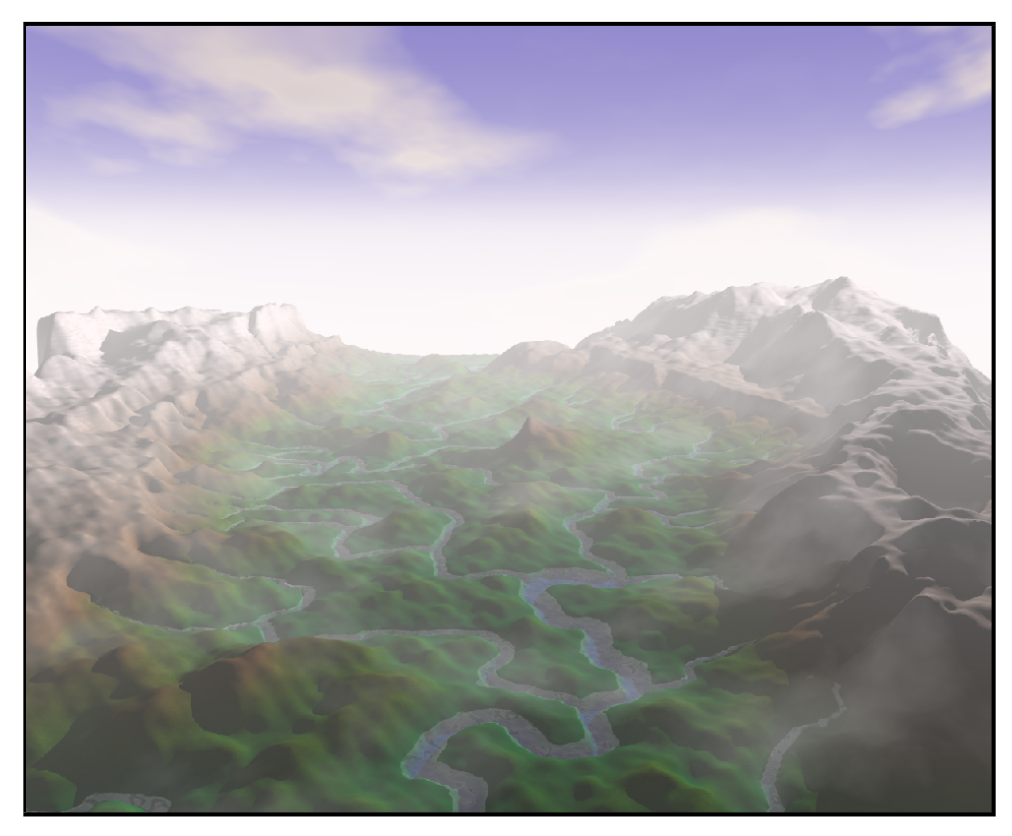
\includegraphics[width=0.6\textwidth]{img/previous_works/belhadj_result.png}
    \caption{Final terrain model generated using a two-step interpolation process (MDI followed by MD), showing smooth integration between fixed ridge and river networks and the surrounding terrain. Source: \cite{Belhadj07}.}
    \label{fig:belhadj_final_result}
\end{figure}

We acknowledge that their method produces highly natural results for river networks, scoring well according to our visual criteria. Their transitions are exceptionally gentle into the river constraints with no noticeable artifacts, demonstrating the effectiveness of their specialised approach for this specific constraint type.

However, our approach demonstrates superior handling of scenarios with \textbf{large height disparities}. While their work does not extensively demonstrate performance with significant elevation differences, our system successfully manages such challenging constraints, as evidenced in our \textit{river network case study} where substantial height variations exist between source and destination points of the river. This capability represents a significant advantage for real-world applications where terrain constraints often involve \textbf{dramatic elevation changes}.

Regarding surrounding terrain quality, we observe that the bottom-up approach, which relies primarily on midpoint displacement and inverse displacement interpolation, lacks the sophisticated \textbf{erosion} and \textbf{detail enhancement} features present in our system. Consequently, while their constraint integration is excellent, the surrounding terrain exhibits less natural variation and detail compared to our results. Our manual approach achieves naturalness levels closely comparable to their specialised method, while our IGA approach, though not quite matching their quality, still produces acceptable results for this constraint type.

\subsection{Comparison with Path-based Constraint Methods}

The path-based terrain generation approach developed by \cite{Andereck14}, shown in Figure \ref{fig:andereck_path}, presents an interesting alternative methodology for handling linear constraints. We compare this with our path/road constraint in Figure \ref{fig:manual_image_1} and Figure \ref{fig:iga_image_1}. 

\begin{figure}[h!]
    \centering
    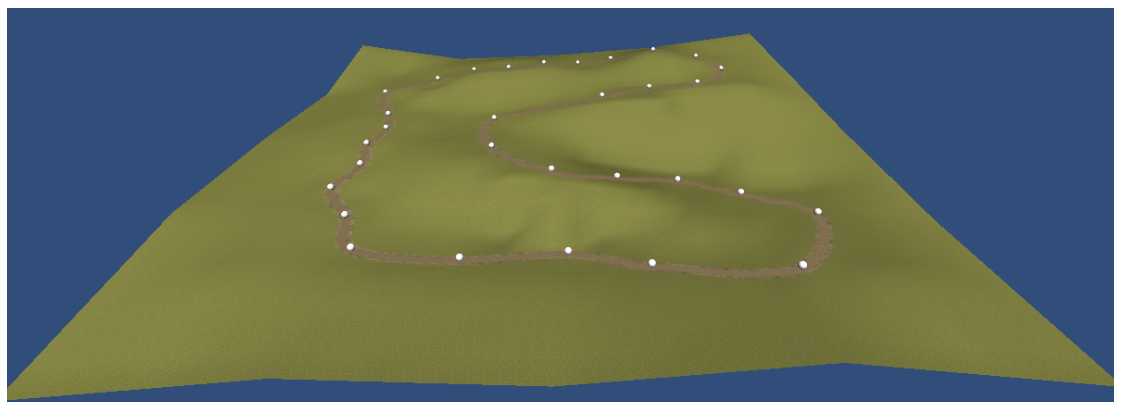
\includegraphics[width=0.6\textwidth]{img/previous_works/adereck_path_result.png}
    \caption{Path-based terrain generation that preserves the exact heights of pre-defined paths while procedurally generating surrounding terrain features. Source: \cite{Andereck14}.}
    \label{fig:andereck_path}
\end{figure}

While their approach demonstrates good transitions and overall natural appearance around the path constraints, we believe our method provides superior results in several key areas. Most notably, our surrounding terrain exhibits significantly greater \textbf{diversity} and \textbf{naturalness}. Their method appears to focus primarily on creating relatively flat terrains around paths that blend smoothly but lack the rich variation and \textit{realistic geological features} that our system produces.

Additionally, our system can adapt to various constraint types beyond just paths, whereas their approach is more specifically tailored to linear path constraints. Even for path-based constraints only, we consider our system to provide a more comprehensive and flexible solution.

\subsection{Manual vs IGA Parameter Tuning}

The comparison between manual parameter adjustment and our Interactive Genetic Algorithm approach reveals important insights about both approaches' capabilities and limitations.

The most significant quality difference between manual and IGA approaches appears in the \textit{river network constraint case study}, where the manual approach (Figure \ref{fig:manual_image_3}) produces more natural-looking terrain compared to the IGA result (Figure \ref{fig:iga_image_3}). This difference highlights that when dealing with complex constraint types requiring nuanced parameter combinations, expert manual tuning can achieve superior results.

However, our evaluation reveals cases where the IGA approach produces preferred results. Notably, in the \textit{island/coastline case study} (Figure \ref{fig:iga_image_4}), we consider the IGA-generated terrain to look better than the manual approach (Figure \ref{fig:manual_image_4}), demonstrating the algorithm's ability to discover unexpected but aesthetically pleasing parameter combinations.

The terrain differences between manual and IGA approaches often reflect genuine variations in aesthetic preference rather than quality deficiencies. The IGA's goal is not to mimic manual expert tuning but to explore the parameter space according to user aesthetic preferences, potentially discovering solutions that manual approaches might not consider.

Manual parameter tuning demonstrates particular advantages when handling constraints with large height disparities. Our IGA system, designed to handle diverse constraint types effectively, prioritises robustness across many normal cases. This design choice means it may struggle with highly specialised scenarios that benefit from expert domain knowledge and targeted parameter selection.

Importantly, both approaches consistently produce results that meet the visual criteria established in Section \ref{visual_crit}. While manual tuning by experts may yield marginally better results in some complex scenarios, the IGA approach successfully democratises the system, enabling non-expert users to achieve satisfactory terrain generation results without requiring deep understanding of the underlying algorithms and parameters.

\section{Performance Evaluation}
\label{performance_eval}

Beyond visual quality assessment, we evaluated the computational performance of our system to understand its practical usability within the Unity development environment. All performance tests were conducted on terrain with a resolution of 1024×1024 heightmap points. Most terrain operations in our system execute with near-instantaneous performance, completing in less than one second. However, certain computationally intensive operations require more detailed performance analysis, which we present in this section.

\subsection{GPU Acceleration Impact}

Our implementation of GPU-accelerated terrain operations demonstrates significant performance improvements over CPU-based alternatives. We evaluated the three primary operations that benefit from GPU acceleration: Basic Smoothing, Enhanced Distance-Based Smoothing, and Thermal Erosion. Each operation was tested using 100 iterations to amplify timing differences and provide measurable performance metrics.

\textbf{GPU Performance:} When utilising compute shader acceleration, all three operations complete their 100-iteration processing in less than one second, demonstrating the substantial computational power available through parallel GPU processing.

\textbf{CPU Performance Comparison:} The CPU fallback implementations, while maintaining algorithmic correctness, exhibit significantly longer processing times:

\begin{itemize}
    \item \textbf{Basic Smoother:} 13 seconds for 100 iterations;
    \item \textbf{Enhanced Distance-Based Smoothing:} 15 seconds for 100 iterations;  
    \item \textbf{Thermal Erosion:} 45 seconds for 100 iterations.
\end{itemize}

The performance difference between GPU and CPU implementations ranges from approximately 13× to over 45× improvement, with thermal erosion showing the most dramatic acceleration. This substantial performance gain demonstrates the effectiveness of our GPU acceleration strategy and justifies the additional implementation complexity.

\textbf{Explaining Performance Differences:} The variation in CPU processing times between operations reflects their computational complexity differences. Basic smoothing performs straightforward neighbourhood averaging, requiring minimal computational overhead per point. Enhanced distance-based smoothing adds distance-aware weight calculations and proximity considerations, resulting in slightly increased processing time.

Thermal erosion exhibits the longest processing time due to its sophisticated material transfer simulation. Unlike simple averaging operations, thermal erosion requires complex neighbour analysis, height difference calculations, and iterative material movement between terrain points. 

\subsection{Interactive Genetic Algorithm Generation Times}

The Interactive Genetic Algorithm component introduces unique performance considerations due to its preview generation requirements. Each terrain genome requires visual preview generation to enable user selection, creating a multiplicative time factor based on population size.

\textbf{Preview Generation Performance:} Individual preview generation averages approximately 5 seconds per genome, with variation ranging from 3 to 8 seconds depending on genome complexity. This variability primarily stems from the number of terrain operations contained within each genome. 

\textbf{Population Size Impact:} The total time required for generating a complete population of terrain previews scales linearly with population size:

\begin{itemize}
    \item \textbf{Population of 8:} Approximately 40 seconds (8 × 5 seconds average)
    \item \textbf{Population of 16:} Approximately 80 seconds (16 × 5 seconds average)  
    \item \textbf{Population of 32:} Approximately 160 seconds (32 × 5 seconds average)
\end{itemize}

While these generation times may initially appear substantial, we consider them acceptable within the context of the IGA's purpose. The Interactive Genetic Algorithm serves to democratise complex terrain generation, enabling non-expert users to achieve sophisticated results without requiring detailed parameter knowledge.

Furthermore, the IGA provides substantial value by exploring parameter combinations that manual approaches might never discover. Users typically require only one high-quality terrain for their specific use case, and once generated, this terrain remains available throughout the development process without requiring regeneration.

The performance characteristics demonstrate that while our Interactive Genetic Algorithm requires meaningful time investment, it provides proportional value through sophisticated parameter exploration and democratised access to complex terrain generation capabilities. For users seeking immediate results, the manual parameter approach remains available with near-instantaneous operation execution.


\section{Summary of Evaluation Results}

Our evaluation across five diverse case studies reveals several key patterns in our system's performance. The distance-based approach consistently excels at creating smooth transitions between fixed and generated terrain, with linear constraints (roads, paths) showing the strongest visual results, while more complex scenarios involving significant height disparities present greater challenges, that our system still overcome. 

The performance analysis reveals a clear trade-off between computational approaches: GPU acceleration provides dramatic speed improvements for intensive operations, while the Interactive Genetic Algorithm introduces longer generation times that are offset by its accessibility to non-expert users. These findings highlight the effectiveness of our hybrid approach, combining rapid individual operations with more time-intensive but intuitive parameter exploration capabilities.





















\chapter*{Conclusion}
\label{epilog}
\addcontentsline{toc}{chapter}{Conclusion}

We conclude that the goals of this thesis were successfully achieved. We presented three key innovations that together solve the constrained terrain generation problem:

\textbf{The Distance-Based Methodology} represents our core technical contribution. We devised a novel approach that treats constraints as \textit{sources} of influence rather than \textit{boundaries} to be joined. By calculating distances from each terrain point to the nearest fixed point, we created a framework for natural transitions. For this, we developed two techniques: \textbf{distance-based height scaling} that adjusts terrain elevations globally, and \textbf{enhanced distance-based smoothing} that preserves detail while ensuring smooth integration into the constraints. The elegance lies in its universality, as our method works with any constraint pattern and any terrain generation algorithm.

\textbf{The Interactive Genetic Algorithm Adaptation} transforms parameter optimisation into visual selection. We adapted existing IGA techniques specifically for our system, introducing crucial innovations in the process. Our idea of a domain-specific initialisation strategy ensures that evolution begins with sensible terrain configurations rather than random ones. Similarly, our specialised and smart mutation operators increase the diversity of solutions to improve generalisation of the constraints that the IGA can handle. These adaptations proved surprisingly effective across diverse constraint types, from road networks to coastlines, and allowed the evolutionary process to provide natural-looking terrains efficiently.

\textbf{The System Implementation} demonstrates our commitment to practical usability. We designed and coded a component-based architecture that separates concerns while enabling GPU acceleration for performance-critical operations. The design allows new algorithms to be added without modifying existing code, while Unity integration provides a familiar environment for developers.

Our system shows particular promise for game development, especially racing games where track layouts must integrate naturally with terrain. By eliminating manual terrain sculpting around predetermined heights, we enable rapid iteration and exploration of design alternatives.

The success of our domain-specific initialisation and mutation strategies suggests broader applications. These techniques could benefit any procedural generation system with subjective quality metrics. Similarly, the distance grid concept invites extensions, perhaps density-based approaches considering constraint concentration rather than just nearest distance, which could create more complex influence patterns.

Through inventing the distance-based approach, implementing an accessible IGA with novel adaptations, and creating a flexible system architecture, we have shown that natural constraint integration is achievable. Our work demonstrates that technical sophistication need not mean user complexity, and that constraints need not constrain creativity.

The true innovation lies not in any single component but in their harmony. The distance-based methodology provides the mathematical foundation, the adapted IGA makes the system accessible, and the modular implementation ensures practical usability. Together, they transform constrained terrain generation from a technical challenge into a creative opportunity.

As virtual worlds grow ever larger and more detailed, we believe our contributions provide both immediate value and a foundation for future innovation. We have created a system where procedural efficiency meets artistic control, where complex algorithms serve intuitive creation, and where fixed constraints become the starting point for natural, beautiful terrains.


Focus on results only. 

%%% Bibliography
\include{bibliography}

%%% Figures used in the thesis (consider if this is needed)
\listoffigures

%%% Tables used in the thesis (consider if this is needed)
%%% In mathematical theses, it could be better to move the list of tables to the beginning of the thesis.
% \listoftables

%%% Abbreviations used in the thesis, if any, including their explanation
%%% In mathematical theses, it could be better to move the list of abbreviations to the beginning of the thesis.
% \chapwithtoc{List of Abbreviations}

%%% Doctoral theses must contain a list of author's publications
\ifx\ThesisType\TypePhD
\chapwithtoc{List of Publications}
\fi

%%% Attachments to the thesis, if any. Each attachment must be referred to
%%% at least once from the text of the thesis. Attachments are numbered.
%%%
%%% The printed version should preferably contain attachments, which can be
%%% read (additional tables and charts, supplementary text, examples of
%%% program output, etc.). The electronic version is more suited for attachments
%%% which will likely be used in an electronic form rather than read (program
%%% source code, data files, interactive charts, etc.). Electronic attachments
%%% should be uploaded to SIS. Allowed file formats are specified in provision
%%% of the rector no. 72/2017. Exceptions can be approved by faculty's coordinator.
\appendix

\chapter{Additional Information}
\label{additional info}


% \section{Hydraulic Erosion Simulation}

\begin{algorithm}[H]
\footnotesize
\centering
\caption{Hydraulic Erosion Simulation}
\label{alg:hydraulic_erosion}
\begin{algorithmic}[1]
\Require $heightMap[width][height]$, $dropletCount$, $erosionStrength$, $solubility$
\Ensure Eroded terrain with water-carved features
\State Initialise $erosionMap[width][height] \leftarrow 0$
\For{$i = 0$ to $dropletCount - 1$}
    \State Choose random starting position $(x, y)$
    \State $erosionMap[x][y] \leftarrow erosionStrength$
    \State $pos \leftarrow (x, y)$
    \While{$erosionMap[pos.x][pos.y] > 0$}
        \State $neighbours \leftarrow$ get valid neighbours of $position$
        \State $foundLower \leftarrow false$
        \For{each $n$ in $neighbors$}
            \If{$heightMap[n.x][n.y] < heightMap[pos.x][pos.y]$}
                \State $erosionMap[n.x][n.y] \leftarrow erosionMap[pos.x][pos.y] - solubility$
                \State $pos \leftarrow n$
                \State $foundLower \leftarrow true$
                \State \textbf{break}
            \EndIf
        \EndFor
        \If{$foundLower = false$}
            \State $erosionMap[pos.x][pos.y] \leftarrow erosionMap[pos.x][pos.y] - solubility$
        \EndIf
    \EndWhile
\EndFor
\State Apply erosion: $heightMap[x][y] \leftarrow heightMap[x][y] - erosionMap[x][y]$
\end{algorithmic}
\end{algorithm}


% \section{Thermal Erosion Simulation}

\begin{algorithm}[h]
\footnotesize
\centering
\caption{Thermal Erosion Simulation}
\label{alg:thermal_erosion}
\begin{algorithmic}[1]
\Require $heightMap[width][height]$, $iterations$, $erosionThreshold$, $erosionRate$
\Ensure Terrain with realistic slope angles
\For{$iter = 0$ to $iterations - 1$}
    \State Create copy $originalMap \leftarrow heightMap$
    \For {$y = 0$ to $height - 1$}
        \For{$x = 0$ to $width - 1$}
            \State $neighbors \leftarrow$ get 8-connected neighbours of $(x, y)$
            \For{each $neighbor$ $(nx, ny)$ in $neighbors$}
                \If{$shouldModify(nx, ny)$}
                    \State $heightDiff \leftarrow originalMap[x][y] - originalMap[nx][ny]$
                    \If{$heightDiff > erosionThreshold$}
                        \State $transferAmount \leftarrow heightDiff \times erosionRate$
                        \State $heightMap[x][y] \leftarrow heightMap[x][y] - transferAmount$
                        \State $heightMap[nx][ny] \leftarrow heightMap[nx][ny] + transferAmount$
                    \EndIf
                \EndIf
            \EndFor
        \EndFor
    \EndFor
\EndFor
\end{algorithmic}
\end{algorithm}

\chapter{Attachments}

The attachments to this thesis contain the complete Unity project and comprehensive documentation for the constrained procedural terrain generation system described throughout the text. The project consists of the following components:

\section{Unity Implementation}

This directory contains the full Unity project for our system, structured as a complete Unity 6 project that can be opened directly in Unity to access all functionality and test scenarios. 

\subsection{Source Code}

The source code: \texttt{Assets/Scripts/TerrainGeneration/} 

The compute shaders: \texttt{Assets/Resources/Shaders/}

\subsection{Test Data and Demonstration Scenes}

The project includes comprehensive test data in \texttt{Assets/TestData/} and multiple demonstration scenes in \texttt{Assets/Scenes/} showcasing various constraint scenarios. Each test scenario includes Unity scene files, constraint mask textures, and pre-configured terrain data assets.

\subsection{Unity Project Configuration}

The project includes complete Unity project settings in \texttt{ProjectSettings/}, package dependencies in \texttt{Packages/}, and render pipeline configurations in \texttt{Assets/Settings/}, allowing the project to be immediately opened directly in Unity 6 or newer.

\subsection{Developer Documentation}
Developer documentation can be seen in \texttt{DEVELOPER\_DOCUMENTATION.md}.

\section{User Documentation}

A comprehensive \texttt{README.md} file provides clear instructions for setting up and using the system in Unity.

\section{Github Repository}
All attachments can also be seen here: \href{https://github.com/Olliewakeford/Procedural-Terrain-Generation-with-fixed-points}{Github Repository Link}


\end{document}
